% Options for packages loaded elsewhere
\PassOptionsToPackage{unicode}{hyperref}
\PassOptionsToPackage{hyphens}{url}
\PassOptionsToPackage{dvipsnames,svgnames,x11names}{xcolor}
%
\documentclass[
  letterpaper,
  DIV=11,
  numbers=noendperiod]{scrreprt}

\usepackage{amsmath,amssymb}
\usepackage{lmodern}
\usepackage{iftex}
\ifPDFTeX
  \usepackage[T1]{fontenc}
  \usepackage[utf8]{inputenc}
  \usepackage{textcomp} % provide euro and other symbols
\else % if luatex or xetex
  \usepackage{unicode-math}
  \defaultfontfeatures{Scale=MatchLowercase}
  \defaultfontfeatures[\rmfamily]{Ligatures=TeX,Scale=1}
\fi
% Use upquote if available, for straight quotes in verbatim environments
\IfFileExists{upquote.sty}{\usepackage{upquote}}{}
\IfFileExists{microtype.sty}{% use microtype if available
  \usepackage[]{microtype}
  \UseMicrotypeSet[protrusion]{basicmath} % disable protrusion for tt fonts
}{}
\makeatletter
\@ifundefined{KOMAClassName}{% if non-KOMA class
  \IfFileExists{parskip.sty}{%
    \usepackage{parskip}
  }{% else
    \setlength{\parindent}{0pt}
    \setlength{\parskip}{6pt plus 2pt minus 1pt}}
}{% if KOMA class
  \KOMAoptions{parskip=half}}
\makeatother
\usepackage{xcolor}
\setlength{\emergencystretch}{3em} % prevent overfull lines
\setcounter{secnumdepth}{5}
% Make \paragraph and \subparagraph free-standing
\ifx\paragraph\undefined\else
  \let\oldparagraph\paragraph
  \renewcommand{\paragraph}[1]{\oldparagraph{#1}\mbox{}}
\fi
\ifx\subparagraph\undefined\else
  \let\oldsubparagraph\subparagraph
  \renewcommand{\subparagraph}[1]{\oldsubparagraph{#1}\mbox{}}
\fi

\usepackage{color}
\usepackage{fancyvrb}
\newcommand{\VerbBar}{|}
\newcommand{\VERB}{\Verb[commandchars=\\\{\}]}
\DefineVerbatimEnvironment{Highlighting}{Verbatim}{commandchars=\\\{\}}
% Add ',fontsize=\small' for more characters per line
\usepackage{framed}
\definecolor{shadecolor}{RGB}{241,243,245}
\newenvironment{Shaded}{\begin{snugshade}}{\end{snugshade}}
\newcommand{\AlertTok}[1]{\textcolor[rgb]{0.68,0.00,0.00}{#1}}
\newcommand{\AnnotationTok}[1]{\textcolor[rgb]{0.37,0.37,0.37}{#1}}
\newcommand{\AttributeTok}[1]{\textcolor[rgb]{0.40,0.45,0.13}{#1}}
\newcommand{\BaseNTok}[1]{\textcolor[rgb]{0.68,0.00,0.00}{#1}}
\newcommand{\BuiltInTok}[1]{\textcolor[rgb]{0.00,0.23,0.31}{#1}}
\newcommand{\CharTok}[1]{\textcolor[rgb]{0.13,0.47,0.30}{#1}}
\newcommand{\CommentTok}[1]{\textcolor[rgb]{0.37,0.37,0.37}{#1}}
\newcommand{\CommentVarTok}[1]{\textcolor[rgb]{0.37,0.37,0.37}{\textit{#1}}}
\newcommand{\ConstantTok}[1]{\textcolor[rgb]{0.56,0.35,0.01}{#1}}
\newcommand{\ControlFlowTok}[1]{\textcolor[rgb]{0.00,0.23,0.31}{#1}}
\newcommand{\DataTypeTok}[1]{\textcolor[rgb]{0.68,0.00,0.00}{#1}}
\newcommand{\DecValTok}[1]{\textcolor[rgb]{0.68,0.00,0.00}{#1}}
\newcommand{\DocumentationTok}[1]{\textcolor[rgb]{0.37,0.37,0.37}{\textit{#1}}}
\newcommand{\ErrorTok}[1]{\textcolor[rgb]{0.68,0.00,0.00}{#1}}
\newcommand{\ExtensionTok}[1]{\textcolor[rgb]{0.00,0.23,0.31}{#1}}
\newcommand{\FloatTok}[1]{\textcolor[rgb]{0.68,0.00,0.00}{#1}}
\newcommand{\FunctionTok}[1]{\textcolor[rgb]{0.28,0.35,0.67}{#1}}
\newcommand{\ImportTok}[1]{\textcolor[rgb]{0.00,0.46,0.62}{#1}}
\newcommand{\InformationTok}[1]{\textcolor[rgb]{0.37,0.37,0.37}{#1}}
\newcommand{\KeywordTok}[1]{\textcolor[rgb]{0.00,0.23,0.31}{#1}}
\newcommand{\NormalTok}[1]{\textcolor[rgb]{0.00,0.23,0.31}{#1}}
\newcommand{\OperatorTok}[1]{\textcolor[rgb]{0.37,0.37,0.37}{#1}}
\newcommand{\OtherTok}[1]{\textcolor[rgb]{0.00,0.23,0.31}{#1}}
\newcommand{\PreprocessorTok}[1]{\textcolor[rgb]{0.68,0.00,0.00}{#1}}
\newcommand{\RegionMarkerTok}[1]{\textcolor[rgb]{0.00,0.23,0.31}{#1}}
\newcommand{\SpecialCharTok}[1]{\textcolor[rgb]{0.37,0.37,0.37}{#1}}
\newcommand{\SpecialStringTok}[1]{\textcolor[rgb]{0.13,0.47,0.30}{#1}}
\newcommand{\StringTok}[1]{\textcolor[rgb]{0.13,0.47,0.30}{#1}}
\newcommand{\VariableTok}[1]{\textcolor[rgb]{0.07,0.07,0.07}{#1}}
\newcommand{\VerbatimStringTok}[1]{\textcolor[rgb]{0.13,0.47,0.30}{#1}}
\newcommand{\WarningTok}[1]{\textcolor[rgb]{0.37,0.37,0.37}{\textit{#1}}}

\providecommand{\tightlist}{%
  \setlength{\itemsep}{0pt}\setlength{\parskip}{0pt}}\usepackage{longtable,booktabs,array}
\usepackage{calc} % for calculating minipage widths
% Correct order of tables after \paragraph or \subparagraph
\usepackage{etoolbox}
\makeatletter
\patchcmd\longtable{\par}{\if@noskipsec\mbox{}\fi\par}{}{}
\makeatother
% Allow footnotes in longtable head/foot
\IfFileExists{footnotehyper.sty}{\usepackage{footnotehyper}}{\usepackage{footnote}}
\makesavenoteenv{longtable}
\usepackage{graphicx}
\makeatletter
\def\maxwidth{\ifdim\Gin@nat@width>\linewidth\linewidth\else\Gin@nat@width\fi}
\def\maxheight{\ifdim\Gin@nat@height>\textheight\textheight\else\Gin@nat@height\fi}
\makeatother
% Scale images if necessary, so that they will not overflow the page
% margins by default, and it is still possible to overwrite the defaults
% using explicit options in \includegraphics[width, height, ...]{}
\setkeys{Gin}{width=\maxwidth,height=\maxheight,keepaspectratio}
% Set default figure placement to htbp
\makeatletter
\def\fps@figure{htbp}
\makeatother
\newlength{\cslhangindent}
\setlength{\cslhangindent}{1.5em}
\newlength{\csllabelwidth}
\setlength{\csllabelwidth}{3em}
\newlength{\cslentryspacingunit} % times entry-spacing
\setlength{\cslentryspacingunit}{\parskip}
\newenvironment{CSLReferences}[2] % #1 hanging-ident, #2 entry spacing
 {% don't indent paragraphs
  \setlength{\parindent}{0pt}
  % turn on hanging indent if param 1 is 1
  \ifodd #1
  \let\oldpar\par
  \def\par{\hangindent=\cslhangindent\oldpar}
  \fi
  % set entry spacing
  \setlength{\parskip}{#2\cslentryspacingunit}
 }%
 {}
\usepackage{calc}
\newcommand{\CSLBlock}[1]{#1\hfill\break}
\newcommand{\CSLLeftMargin}[1]{\parbox[t]{\csllabelwidth}{#1}}
\newcommand{\CSLRightInline}[1]{\parbox[t]{\linewidth - \csllabelwidth}{#1}\break}
\newcommand{\CSLIndent}[1]{\hspace{\cslhangindent}#1}

\KOMAoption{captions}{tableheading}
\makeatletter
\@ifpackageloaded{tcolorbox}{}{\usepackage[many]{tcolorbox}}
\@ifpackageloaded{fontawesome5}{}{\usepackage{fontawesome5}}
\definecolor{quarto-callout-color}{HTML}{909090}
\definecolor{quarto-callout-note-color}{HTML}{0758E5}
\definecolor{quarto-callout-important-color}{HTML}{CC1914}
\definecolor{quarto-callout-warning-color}{HTML}{EB9113}
\definecolor{quarto-callout-tip-color}{HTML}{00A047}
\definecolor{quarto-callout-caution-color}{HTML}{FC5300}
\definecolor{quarto-callout-color-frame}{HTML}{acacac}
\definecolor{quarto-callout-note-color-frame}{HTML}{4582ec}
\definecolor{quarto-callout-important-color-frame}{HTML}{d9534f}
\definecolor{quarto-callout-warning-color-frame}{HTML}{f0ad4e}
\definecolor{quarto-callout-tip-color-frame}{HTML}{02b875}
\definecolor{quarto-callout-caution-color-frame}{HTML}{fd7e14}
\makeatother
\makeatletter
\makeatother
\makeatletter
\@ifpackageloaded{bookmark}{}{\usepackage{bookmark}}
\makeatother
\makeatletter
\@ifpackageloaded{caption}{}{\usepackage{caption}}
\AtBeginDocument{%
\ifdefined\contentsname
  \renewcommand*\contentsname{Table of contents}
\else
  \newcommand\contentsname{Table of contents}
\fi
\ifdefined\listfigurename
  \renewcommand*\listfigurename{List of Figures}
\else
  \newcommand\listfigurename{List of Figures}
\fi
\ifdefined\listtablename
  \renewcommand*\listtablename{List of Tables}
\else
  \newcommand\listtablename{List of Tables}
\fi
\ifdefined\figurename
  \renewcommand*\figurename{Figure}
\else
  \newcommand\figurename{Figure}
\fi
\ifdefined\tablename
  \renewcommand*\tablename{Table}
\else
  \newcommand\tablename{Table}
\fi
}
\@ifpackageloaded{float}{}{\usepackage{float}}
\floatstyle{ruled}
\@ifundefined{c@chapter}{\newfloat{codelisting}{h}{lop}}{\newfloat{codelisting}{h}{lop}[chapter]}
\floatname{codelisting}{Listing}
\newcommand*\listoflistings{\listof{codelisting}{List of Listings}}
\makeatother
\makeatletter
\@ifpackageloaded{caption}{}{\usepackage{caption}}
\@ifpackageloaded{subcaption}{}{\usepackage{subcaption}}
\makeatother
\makeatletter
\@ifpackageloaded{tcolorbox}{}{\usepackage[many]{tcolorbox}}
\makeatother
\makeatletter
\@ifundefined{shadecolor}{\definecolor{shadecolor}{rgb}{.97, .97, .97}}
\makeatother
\makeatletter
\makeatother
\ifLuaTeX
  \usepackage{selnolig}  % disable illegal ligatures
\fi
\IfFileExists{bookmark.sty}{\usepackage{bookmark}}{\usepackage{hyperref}}
\IfFileExists{xurl.sty}{\usepackage{xurl}}{} % add URL line breaks if available
\urlstyle{same} % disable monospaced font for URLs
\hypersetup{
  pdftitle={RwithSLING},
  pdfauthor={Bo Burla},
  colorlinks=true,
  linkcolor={blue},
  filecolor={Maroon},
  citecolor={Blue},
  urlcolor={Blue},
  pdfcreator={LaTeX via pandoc}}

\title{RwithSLING}
\author{Bo Burla}
\date{5/13/2022}

\begin{document}
\maketitle
\ifdefined\Shaded\renewenvironment{Shaded}{\begin{tcolorbox}[frame hidden, sharp corners, borderline west={3pt}{0pt}{shadecolor}, breakable, boxrule=0pt, interior hidden, enhanced]}{\end{tcolorbox}}\fi

\renewcommand*\contentsname{Table of contents}
{
\hypersetup{linkcolor=}
\setcounter{tocdepth}{2}
\tableofcontents
}
\bookmarksetup{startatroot}

\hypertarget{welcome}{%
\chapter*{Welcome}\label{welcome}}
\addcontentsline{toc}{chapter}{Welcome}

This online book aims to provide an applied quick-start introduction
into the processing, management, and analysis of mass spectrometry
(MS)-based lipidomics datasets and associated study metadata using R.

The books is structured into two parts: (i) \textbf{Tutorials} introduce
a few basic but applied concepts of using R , and (ii) \textbf{Recipes}
provide workflows and sample code for data processing, and data analysis
and visualization tasks frequently used in the lab.

This book was and is mainly written during the RwithSLING workshop
sessions at SLING that started in 2022.

Feedback and contributions are very welcome!

\hypertarget{acknowledgements}{%
\section*{Acknowledgements}\label{acknowledgements}}
\addcontentsline{toc}{section}{Acknowledgements}

\bookmarksetup{startatroot}

\hypertarget{sec-intro}{%
\chapter{Introduction}\label{sec-intro}}

\hypertarget{prerequisites}{%
\section{Prerequisites}\label{prerequisites}}

Following software need to be installed on your computer to work with
the examples shown in this online book:

\begin{itemize}
\item
  \texttt{R} Version 4.1 (or higher) \url{https://cloud.r-project.org/}.
  Check your R version by running following command in your console:

\begin{Shaded}
\begin{Highlighting}[]
\FunctionTok{R.Version}\NormalTok{()}\SpecialCharTok{$}\NormalTok{version.string}
\end{Highlighting}
\end{Shaded}

\begin{verbatim}
#> [1] "R version 4.2.0 (2022-04-22 ucrt)"
\end{verbatim}
\item
  \texttt{RStudio} Version 2022.02 or higher
  \url{https://www.rstudio.com/products/rstudio/download/\#download}.
  Check your \texttt{RStudio} version by either looking clicking
  \emph{About RStudio} under the menu \emph{Help}, or by running
  following command in your console

\begin{Shaded}
\begin{Highlighting}[]
\NormalTok{rstudioapi}\SpecialCharTok{::}\FunctionTok{versionInfo}\NormalTok{()}\SpecialCharTok{$}\NormalTok{version}
\end{Highlighting}
\end{Shaded}
\end{itemize}

Following software are only needed for specific chapters/examples:

\begin{itemize}
\tightlist
\item
  \texttt{Git} \url{https://git-scm.com/downloads}
\item
  For Windows: \texttt{Rtools}
  \textless https://cran.r-project.org/bin/windows/Rtools/
\end{itemize}

\hypertarget{frequently-used-r-packages}{%
\section{Frequently used R packages}\label{frequently-used-r-packages}}

See also @ref(Installing R packages)

Following R packages will be often used in the given examples and it is
thus recommended to install them before starting with this book

\begin{itemize}
\tightlist
\item
  \texttt{here}
\item
  \texttt{tidyverse}(installs
  \texttt{ggplot2,\ dplyr,\ tidyr,\ tibble,\ readr,\ forcats,\ stringr,\ purrr})
\item
  \texttt{readxl}
\item
  \texttt{remotes}
\end{itemize}

Run this in your R command line to install these packages:

\begin{Shaded}
\begin{Highlighting}[]
\NormalTok{pkg\_list }\OtherTok{\textless{}{-}} \FunctionTok{c}\NormalTok{(}\StringTok{"here"}\NormalTok{, }\StringTok{"tidyverse"}\NormalTok{, }\StringTok{"readxl"}\NormalTok{, }\StringTok{"remotes"}\NormalTok{)}
\FunctionTok{install.packages}\NormalTok{(pkg\_list)}
\end{Highlighting}
\end{Shaded}

\part{Tutorials}

\hypertarget{import-data-into-r}{%
\chapter{Import data into R}\label{import-data-into-r}}

\hypertarget{introduction}{%
\section{Introduction}\label{introduction}}

\begin{tcolorbox}[enhanced jigsaw, colframe=quarto-callout-note-color-frame, breakable, bottomrule=.15mm, left=2mm, arc=.35mm, leftrule=.75mm, rightrule=.15mm, toprule=.15mm, opacityback=0, colback=white]
\begin{minipage}[t]{5.5mm}
\textcolor{quarto-callout-note-color}{\faInfo}
\end{minipage}%
\begin{minipage}[t]{\textwidth - 5.5mm}
Verify the integrity of your data files and imported data - do not just
assume all is fine\end{minipage}%
\end{tcolorbox}

Data analysis projects often start by importing data from files. It is
easier to start with clearly structured, clean and consistent data
files:

\begin{itemize}
\tightlist
\item
  Tidy data: \emph{observations} (e.g.~samples) as \emph{rows},
  \emph{variables} (e.g.~compounds) as \emph{columns}
\item
  First row contains column names
\item
  No nested columns and rows
\item
  No text before and after the table
\end{itemize}

We will be using \texttt{readr} (from tidyverse) and \texttt{readxl}
packages in this chapter:

\begin{Shaded}
\begin{Highlighting}[]
\FunctionTok{library}\NormalTok{(here)}
\FunctionTok{library}\NormalTok{(tidyverse)}
\FunctionTok{library}\NormalTok{(readxl)}
\end{Highlighting}
\end{Shaded}

\hypertarget{read-csv-files}{%
\section{Read CSV files}\label{read-csv-files}}

\textbf{Hint}: Inspect the summery provided by \texttt{read\_csv()} to
verify correct data types were assigned

\begin{Shaded}
\begin{Highlighting}[]
\NormalTok{d\_wide }\OtherTok{\textless{}{-}} \FunctionTok{read\_csv}\NormalTok{(}\AttributeTok{file =} \FunctionTok{here}\NormalTok{(}\StringTok{"data/Testdata\_Lipidomics\_flat\_wide\_V2.csv"}\NormalTok{), }
                   \AttributeTok{col\_names =} \ConstantTok{TRUE}\NormalTok{, }
                   \AttributeTok{trim\_ws =} \ConstantTok{TRUE}\NormalTok{)}
\end{Highlighting}
\end{Shaded}

\begin{verbatim}
#> Rows: 215 Columns: 430
#> -- Column specification --------------------------------------------------------
#> Delimiter: ","
#> chr    (3): DataFileme, SPLType, VialPosition
#> dbl  (426): CE 14:0, CE 15:0, CE 16:0, CE 16:1, CE 16:2, CE 17:0, CE 17:1, C...
#> dttm   (1): AcqTimeStamp
#> 
#> i Use `spec()` to retrieve the full column specification for this data.
#> i Specify the column types or set `show_col_types = FALSE` to quiet this message.
\end{verbatim}

To remove white-spaces before and after text, set
\texttt{trim\_ws\ =\ TRUE}.

\hypertarget{read-excel-tables}{%
\section{Read Excel tables}\label{read-excel-tables}}

Importing Excel tables can be done via the package s \texttt{readxl}.
Note: you will need to define which sheet to import (e.g.~below
\texttt{Sheet1}).

\begin{Shaded}
\begin{Highlighting}[]
\FunctionTok{library}\NormalTok{(readxl)}
\NormalTok{d\_wide }\OtherTok{\textless{}{-}} \FunctionTok{read\_xlsx}\NormalTok{(}\AttributeTok{path =}\NormalTok{ here}\SpecialCharTok{::}\FunctionTok{here}\NormalTok{(}\StringTok{"data/Testdata\_Lipidomics\_flat\_wide\_V2.xlsx"}\NormalTok{),}
                            \AttributeTok{sheet =} \StringTok{"Sheet1"}\NormalTok{,}
                            \AttributeTok{trim\_ws =} \ConstantTok{TRUE}\NormalTok{, }
                            \AttributeTok{na =} \FunctionTok{c}\NormalTok{(}\StringTok{"ND"}\NormalTok{))}
\FunctionTok{print}\NormalTok{(d\_wide)}
\end{Highlighting}
\end{Shaded}

\begin{verbatim}
#> # A tibble: 215 x 432
#>   DataFileName          AcqTimeStamp SampleType VialPosition `CE 14:0` `CE 15:0`
#>   <chr>                 <chr>        <chr>      <chr>            <dbl>     <dbl>
#> 1 001_EQC_TQC prerun 0~ 2018-04-12T~ EQC        Vial 2            1532       515
#> 2 002_EQC_TQC prerun 0~ 2018-04-12T~ EQC        Vial 2            1029       911
#> 3 003_EQC_TQC prerun 0~ 2018-04-12T~ EQC        Vial 2             685       649
#> 4 004_EQC_TQC prerun 0~ 2018-04-12T~ EQC        Vial 2            1283       576
#> 5 005_EQC_TQC prerun 0~ 2018-04-12T~ EQC        Vial 2             946       732
#> 6 006_EBLK_Extracted B~ 2018-04-12T~ PBLK       P1-A1              132        NA
#> # ... with 209 more rows, and 426 more variables: `CE 16:0` <dbl>,
#> #   `CE 16:1` <dbl>, `CE 16:2` <dbl>, `CE 17:0` <chr>, `CE 17:1` <dbl>,
#> #   `CE 18:0` <dbl>, `CE 18:1` <dbl>, `CE 18:1 d7 (ISTD)` <dbl>, ...
\end{verbatim}

\begin{tcolorbox}[enhanced jigsaw, coltitle=black, breakable, bottomrule=.15mm, left=2mm, arc=.35mm, colbacktitle=quarto-callout-note-color!10!white, leftrule=.75mm, colframe=quarto-callout-note-color-frame, colback=white, title=\textcolor{quarto-callout-note-color}{\faInfo}\hspace{0.5em}{Verify integrity of imported data}, titlerule=0mm, opacitybacktitle=0.6, rightrule=.15mm, bottomtitle=1mm, toptitle=1mm, opacityback=0, toprule=.15mm]

\begin{itemize}
\tightlist
\item
  Do not assume imported data fine without having reason to do so
\item
  Ensure data types were correctly assigned
\item
  Ensure missing values are correctly handled
\end{itemize}

\end{tcolorbox}

\hypertarget{data-types}{%
\section{Data Types}\label{data-types}}

\begin{itemize}
\tightlist
\item
  \textbf{Note:} \texttt{read\_csv()} or \texttt{read\_xlsx()} will by
  default \textbf{\emph{guess}} the data type of each column.
\item
  Typical data types are numbers (\texttt{dbl}), text (\texttt{chr}),
  logical (\texttt{lgl}) and factor (\texttt{fct})
\item
  You can define the column types already at import (see
  \texttt{?read\_csv}).
\end{itemize}

\hypertarget{missing-values}{%
\section{Missing Values}\label{missing-values}}

\begin{itemize}
\tightlist
\item
  Data files often contain missing values, i.e.~as empty cells.
\item
  \texttt{read\_csv()} or \texttt{read\_xlsx()} assign empty/missing
  values as \texttt{NA} (\emph{Not Available}).
\item
  Missing values will in general not affect to data type guessed by
  \texttt{read\_csv()}
\item
  Exception: Column contains only massing values, in this case it will
  be of type \texttt{logical}
\item
  However, if data files contain specific text values for missing values
  (e.g.,``\emph{ND''},''\emph{LOD''}, \emph{``na'')}, then
  \texttt{read\_csv()} or \texttt{read\_xlsx()} assign the column by
  default as character (text)
\end{itemize}

Results from e.g.~clinical chemistry, frequently indicate not available
data with a short text such as \emph{``clotted''}, \emph{``hemolytic''},
\emph{``no received''} to explain why a value was not reported. What
happens when we import such a file using \texttt{read\_csv} with default
parameters:

\begin{Shaded}
\begin{Highlighting}[]
\NormalTok{data\_file\_path }\OtherTok{\textless{}{-}}\NormalTok{ here}\SpecialCharTok{::}\FunctionTok{here}\NormalTok{(}\StringTok{"data/Testdata\_Lipidomics\_flat\_wide\_with\_differentNA\_V2.csv"}\NormalTok{)}
\NormalTok{d\_wide }\OtherTok{\textless{}{-}}\NormalTok{ readr}\SpecialCharTok{::}\FunctionTok{read\_csv}\NormalTok{(data\_file\_path, }\AttributeTok{trim\_ws =} \ConstantTok{TRUE}\NormalTok{)}
\end{Highlighting}
\end{Shaded}

\begin{verbatim}
#> Rows: 215 Columns: 432
#> -- Column specification --------------------------------------------------------
#> Delimiter: ","
#> chr  (109): DataFileNDme, SampleType, VialPosition, CE 15:0, CE 16:0, CE 17:...
#> dbl  (320): CE 14:0, CE 16:1, CE 17:1, CE 18:0, CE 18:1, CE 18:1 d7 (ISTD), ...
#> lgl    (2): CE 16:2, LPC 16:0
#> dttm   (1): AcqTimeStamp
#> 
#> i Use `spec()` to retrieve the full column specification for this data.
#> i Specify the column types or set `show_col_types = FALSE` to quiet this message.
\end{verbatim}

\begin{itemize}
\tightlist
\item
  \texttt{read\_csv()} was mislead by the presence of unknown text
  values and guessed the data types wrongly as
  \texttt{\textless{}char\textgreater{}} for some columns.
\item
  We also have two columns of the type
  \texttt{\textless{}lgl\textgreater{}}, which stand for logical
  (\texttt{TRUE}/\texttt{FALSE}). In this case all peak areas of CE 16:2
  were missing, and \texttt{read\_csv} has no way to guess the intended
  data type. In which case it chooses
  \texttt{\textless{}lgl\textgreater{}} will be chosen as default.
\item
  We will not be able to perform any calculations for columns that are
  text or logical.
\item
  We need to explicitly tell R which values to interpret as missing
  values (\texttt{NA}).
\item
  We can do by providing the \texttt{na} parameter a list of texts that
  should be interpreted as \texttt{NA} :
\end{itemize}

\begin{Shaded}
\begin{Highlighting}[]
\NormalTok{data\_file\_path }\OtherTok{\textless{}{-}}\NormalTok{ here}\SpecialCharTok{::}\FunctionTok{here}\NormalTok{(}\StringTok{"data/Testdata\_Lipidomics\_flat\_wide\_with\_differentNA\_V2.csv"}\NormalTok{)}
\NormalTok{d\_wide }\OtherTok{\textless{}{-}}\NormalTok{ readr}\SpecialCharTok{::}\FunctionTok{read\_csv}\NormalTok{(data\_file\_path, }
                          \AttributeTok{trim\_ws =} \ConstantTok{TRUE}\NormalTok{, }
                          \AttributeTok{na =} \FunctionTok{c}\NormalTok{(}\StringTok{"ND"}\NormalTok{, }\StringTok{"LOD"}\NormalTok{))}
\end{Highlighting}
\end{Shaded}

\begin{verbatim}
#> Warning: One or more parsing issues, see `problems()` for details
\end{verbatim}

\begin{verbatim}
#> Rows: 215 Columns: 432
#> -- Column specification --------------------------------------------------------
#> Delimiter: ","
#> chr    (3): DataFileNDme, SampleType, VialPosition
#> dbl  (425): CE 14:0, CE 15:0, CE 16:0, CE 16:1, CE 17:0, CE 17:1, CE 18:0, C...
#> lgl    (3): CE 16:2, Cer d18:2/24:0, LPC 16:0
#> dttm   (1): AcqTimeStamp
#> 
#> i Use `spec()` to retrieve the full column specification for this data.
#> i Specify the column types or set `show_col_types = FALSE` to quiet this message.
\end{verbatim}

\begin{Shaded}
\begin{Highlighting}[]
\FunctionTok{print}\NormalTok{(d\_wide)}
\end{Highlighting}
\end{Shaded}

\begin{verbatim}
#> # A tibble: 215 x 432
#>   DataFileNDme   AcqTimeStamp        SampleType VialPosition `CE 14:0` `CE 15:0`
#>   <chr>          <dttm>              <chr>      <chr>            <dbl>     <dbl>
#> 1 001_EQC_TQC p~ 2018-04-12 18:28:00 EQC        Vial 2            1532       515
#> 2 002_EQC_TQC p~ 2018-04-12 18:39:00 EQC        Vial 2            1029        NA
#> 3 003_EQC_TQC p~ 2018-04-12 18:51:00 EQC        Vial 2             685       649
#> 4 004_EQC_TQC p~ 2018-04-12 19:02:00 EQC        Vial 2            1283       576
#> 5 005_EQC_TQC p~ 2018-04-12 19:13:00 EQC        Vial 2             946       732
#> 6 006_EBLK_Extr~ 2018-04-12 19:25:00 PBLK       P1-A1              132        NA
#> # ... with 209 more rows, and 426 more variables: `CE 16:0` <dbl>,
#> #   `CE 16:1` <dbl>, `CE 16:2` <lgl>, `CE 17:0` <dbl>, `CE 17:1` <dbl>,
#> #   `CE 18:0` <dbl>, `CE 18:1` <dbl>, `CE 18:1 d7 (ISTD)` <dbl>, ...
\end{verbatim}

\hypertarget{other-considerations}{%
\section{Other Considerations}\label{other-considerations}}

\begin{itemize}
\tightlist
\item
  White spaces or double spaces, White spaces before or after text
  fields can (and often will) cause issues downstream, therefore I
  suggest to trim whitespaces, e.g.~by setting
  \texttt{trim\_ws\ =\ TRUE}
\end{itemize}

\hypertarget{tables-in-r}{%
\chapter{Tables in R}\label{tables-in-r}}

\hypertarget{introduction-1}{%
\section{Introduction}\label{introduction-1}}

In this chapter we will look at how data is used and managed within R.

\hypertarget{prerequisites-1}{%
\subsection{Prerequisites}\label{prerequisites-1}}

\begin{Shaded}
\begin{Highlighting}[]
\FunctionTok{library}\NormalTok{(here)}
\FunctionTok{library}\NormalTok{(tidyverse)}
\end{Highlighting}
\end{Shaded}

\hypertarget{base}{%
\subsubsection{Base}\label{base}}

\begin{Shaded}
\begin{Highlighting}[]
\FunctionTok{plot}\NormalTok{(cars)}
\end{Highlighting}
\end{Shaded}

\begin{figure}[H]

{\centering 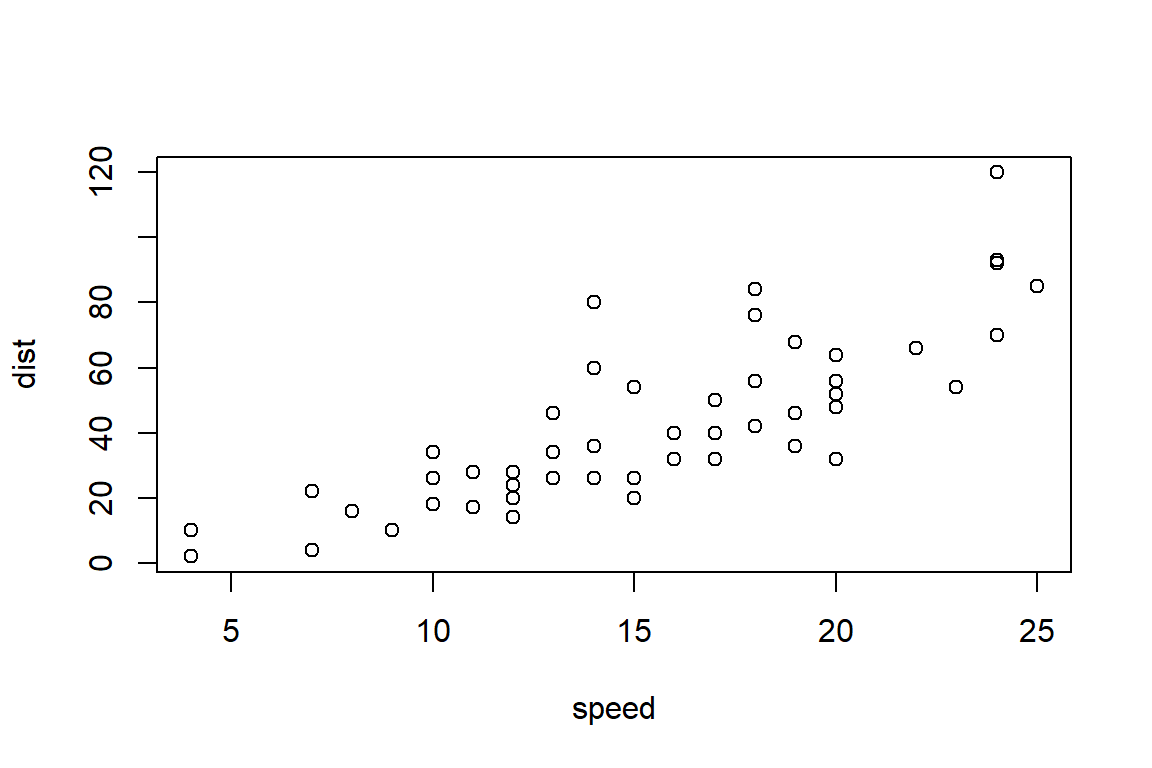
\includegraphics[width=18.75in,height=\textheight]{./tables_files/figure-pdf/unnamed-chunk-3-1.pdf}

}

\end{figure}

\hypertarget{ggplot2}{%
\subsubsection{ggplot2}\label{ggplot2}}

\begin{Shaded}
\begin{Highlighting}[]
\FunctionTok{ggplot}\NormalTok{(}\AttributeTok{data =}\NormalTok{ cars, }\FunctionTok{aes}\NormalTok{(}\AttributeTok{x =}\NormalTok{ speed, }\AttributeTok{y =}\NormalTok{ dist)) }\SpecialCharTok{+} \FunctionTok{geom\_point}\NormalTok{()}
\end{Highlighting}
\end{Shaded}

\begin{figure}[H]

{\centering \includegraphics[width=18.75in,height=\textheight]{./tables_files/figure-pdf/unnamed-chunk-4-1.pdf}

}

\end{figure}

\hypertarget{important-r-data-formats}{%
\section{Important R data formats}\label{important-r-data-formats}}

\begin{longtable}[]{@{}
  >{\raggedright\arraybackslash}p{(\columnwidth - 4\tabcolsep) * \real{0.0686}}
  >{\raggedright\arraybackslash}p{(\columnwidth - 4\tabcolsep) * \real{0.3824}}
  >{\raggedright\arraybackslash}p{(\columnwidth - 4\tabcolsep) * \real{0.5490}}@{}}
\toprule()
\begin{minipage}[b]{\linewidth}\raggedright
Type
\end{minipage} & \begin{minipage}[b]{\linewidth}\raggedright
Description
\end{minipage} & \begin{minipage}[b]{\linewidth}\raggedright
Example(s)
\end{minipage} \\
\midrule()
\endhead
Vector & Vector (series) of values. All values are of the same data type
(see below) &
\texttt{c(1,2,3,4)c("TQC",\ "BQC",\ "SPL")c(TRUE,\ FALSE)} \\
Matrix & 2-dimensional set of values. All values are of the same data
type &
\texttt{matrix(data\ =\ c(1:2),nrow\ =\ 2,ncol\ =\ 3)matrix(data\ =\ c("BQC",\ "SPL"),nrow\ =\ 2,ncol\ =\ 3)} \\
\begin{minipage}[t]{\linewidth}\raggedright
Data Frame\\
Tibble\strut
\end{minipage} & Table with columns that can have different data types &
\texttt{tibble(\ \ \ No\ =\ c(1,2,3),\ \ \ \ Sample\ =\ c("SPL\_1",\ "SPL\_2",\ "SPL\_3"))} \\
List & Series of objects &
\texttt{list(\ \ \ Studysite\ =\ c("NUH",\ "SGH"),\ \ \ Cohort\ =\ \ \ \ \ \ tibble(No\ =\ c(1,2),\ \ \ \ \ \ \ \ \ \ \ \ \ Size\ =\ c(110,332)\ \ \ ))} \\
\bottomrule()
\end{longtable}

\hypertarget{important-r-data-types}{%
\section{Important R data types}\label{important-r-data-types}}

\begin{longtable}[]{@{}
  >{\raggedright\arraybackslash}p{(\columnwidth - 6\tabcolsep) * \real{0.2400}}
  >{\raggedright\arraybackslash}p{(\columnwidth - 6\tabcolsep) * \real{0.1333}}
  >{\raggedright\arraybackslash}p{(\columnwidth - 6\tabcolsep) * \real{0.3333}}
  >{\raggedright\arraybackslash}p{(\columnwidth - 6\tabcolsep) * \real{0.2933}}@{}}
\toprule()
\begin{minipage}[b]{\linewidth}\raggedright
Type
\end{minipage} & \begin{minipage}[b]{\linewidth}\raggedright
Short
\end{minipage} & \begin{minipage}[b]{\linewidth}\raggedright
Description
\end{minipage} & \begin{minipage}[b]{\linewidth}\raggedright
Example(s)
\end{minipage} \\
\midrule()
\endhead
Numeric (double) & \texttt{\textless{}dbl\textgreater{}} & Floating
point number & \texttt{3.14159} \\
Character & \texttt{\textless{}char\textgreater{}} & Character (text)
string & \texttt{"S1P\ d18:1",\ "BQC"} \\
Logical & \texttt{\textless{}lgl\textgreater{}} & True or False, 1 or 0
& \texttt{TRUE;\ FALSE} \\
Integer & \texttt{\textless{}int\textgreater{}} & Number without digits
& \texttt{3L;\ 7011L;\ -13L} \\
Factor & \texttt{\textless{}fct\textgreater{}} & Categorical data &
\texttt{BQC;\ TQC;\ SPL} \\
\bottomrule()
\end{longtable}

Moreover there are data and time types, i.e.~date
\texttt{\textless{}dt\textgreater{}}, time
\texttt{\textless{}tm\textgreater{}} and datetime
\texttt{\textless{}dttm\textgreater{}}

You can print tables in the console or in R notebook (.Rmd), which will
also show the column types:

\hypertarget{select-and-plot}{%
\chapter{Select and plot}\label{select-and-plot}}

\hypertarget{introduction-2}{%
\section{Introduction}\label{introduction-2}}

In this chapter we will look at how read data from files into R \#\#\#
Prerequisites

\begin{Shaded}
\begin{Highlighting}[]
\FunctionTok{library}\NormalTok{(here)}
\FunctionTok{library}\NormalTok{(tidyverse)}
\FunctionTok{library}\NormalTok{(SLINGtools)}
\end{Highlighting}
\end{Shaded}

\hypertarget{import-an-agilent-masshunter-csv-file}{%
\section{Import an Agilent MassHunter CSV
file}\label{import-an-agilent-masshunter-csv-file}}

\begin{Shaded}
\begin{Highlighting}[]
\NormalTok{data\_file\_path }\OtherTok{\textless{}{-}} \FunctionTok{here}\NormalTok{(}\StringTok{"data/Testdata\_Lipidomics\_MHQuant\_Detailed\_V2.csv"}\NormalTok{)}

\NormalTok{d\_orig }\OtherTok{\textless{}{-}} \FunctionTok{read\_MassHunterCSV}\NormalTok{(data\_file\_path)}
\end{Highlighting}
\end{Shaded}

\begin{verbatim}
#> Reading 'Testdata_Lipidomics_MHQuant_Detailed_V2.csv' ... 
#> 
indexing Testdata_Lipidomics_MHQuant_Detailed_V2.csv [======] 2.15GB/s, eta:  0s
                                                                                
Imported  215 samples with 428 transitions
\end{verbatim}

\begin{Shaded}
\begin{Highlighting}[]
\FunctionTok{print}\NormalTok{(d\_orig)}
\end{Highlighting}
\end{Shaded}

\begin{verbatim}
#> # A tibble: 92,020 x 14
#>   DataFileName      DataName SampleType AcqTimeStamp        VialPosition Feature
#>   <chr>             <chr>    <chr>      <dttm>              <chr>        <chr>  
#> 1 001_EQC_TQC prer~ 001_EQC~ EQC        2018-04-12 18:28:00 Vial 2       CE 14:0
#> 2 001_EQC_TQC prer~ 001_EQC~ EQC        2018-04-12 18:28:00 Vial 2       CE 15:0
#> 3 001_EQC_TQC prer~ 001_EQC~ EQC        2018-04-12 18:28:00 Vial 2       CE 16:0
#> 4 001_EQC_TQC prer~ 001_EQC~ EQC        2018-04-12 18:28:00 Vial 2       CE 16:1
#> 5 001_EQC_TQC prer~ 001_EQC~ EQC        2018-04-12 18:28:00 Vial 2       CE 16:2
#> 6 001_EQC_TQC prer~ 001_EQC~ EQC        2018-04-12 18:28:00 Vial 2       CE 17:0
#> # ... with 92,014 more rows, and 8 more variables: IonPolarity <fct>,
#> #   PrecursorMZ <dbl>, ProductMZ <dbl>, CollisionEnergy <dbl>, RT <dbl>,
#> #   Area <dbl>, FWHM <dbl>, MI <lgl>
\end{verbatim}

\hypertarget{select-remove-re-order-and-rename-columns}{%
\section{Select, remove, re-order, and rename
columns}\label{select-remove-re-order-and-rename-columns}}

Use the function \texttt{select()}

\begin{Shaded}
\begin{Highlighting}[]
\NormalTok{d }\OtherTok{\textless{}{-}}\NormalTok{ d\_orig }\SpecialCharTok{|\textgreater{}} 
\NormalTok{  dplyr}\SpecialCharTok{::}\FunctionTok{select}\NormalTok{(}\AttributeTok{AnalysisID =} \StringTok{"DataFileName"}\NormalTok{, }
                \AttributeTok{QCtype =}\NormalTok{ SampleType,}
                \AttributeTok{Compound =}\NormalTok{ Feature, }
                \AttributeTok{Intensity =}\NormalTok{ Area,}
\NormalTok{                RT,}
\NormalTok{                PrecursorMZ)}
\FunctionTok{print}\NormalTok{(d)}
\end{Highlighting}
\end{Shaded}

\begin{verbatim}
#> # A tibble: 92,020 x 6
#>   AnalysisID              QCtype Compound Intensity    RT PrecursorMZ
#>   <chr>                   <chr>  <chr>        <dbl> <dbl>       <dbl>
#> 1 001_EQC_TQC prerun 01.d EQC    CE 14:0       1532  6.98        615.
#> 2 001_EQC_TQC prerun 01.d EQC    CE 15:0        515  7.13        629.
#> 3 001_EQC_TQC prerun 01.d EQC    CE 16:0     127953  7.16        643.
#> 4 001_EQC_TQC prerun 01.d EQC    CE 16:1      40374  7.00        641.
#> 5 001_EQC_TQC prerun 01.d EQC    CE 16:2       1340  6.82        639.
#> 6 001_EQC_TQC prerun 01.d EQC    CE 17:0       7227  7.22        657.
#> # ... with 92,014 more rows
\end{verbatim}

\hypertarget{filter-rows}{%
\section{Filter rows}\label{filter-rows}}

Use the function \texttt{filter()}.

\begin{Shaded}
\begin{Highlighting}[]
\NormalTok{d }\SpecialCharTok{|\textgreater{}} \FunctionTok{filter}\NormalTok{(AnalysisID }\SpecialCharTok{==} \StringTok{"149\_BQC\_PQC17.d "}\NormalTok{)}
\NormalTok{d }\SpecialCharTok{|\textgreater{}} \FunctionTok{filter}\NormalTok{(AnalysisID }\SpecialCharTok{==} \StringTok{"149{-}bQC\_PQC17.d"}\NormalTok{, Compound }\SpecialCharTok{==} \StringTok{"TG 48:1 [{-}18:1]"}\NormalTok{)}
\NormalTok{d }\SpecialCharTok{|\textgreater{}} \FunctionTok{filter}\NormalTok{(QCtype }\SpecialCharTok{==} \StringTok{"BQC"}\NormalTok{)}
\NormalTok{d }\SpecialCharTok{|\textgreater{}} \FunctionTok{filter}\NormalTok{(QCtype }\SpecialCharTok{==} \StringTok{"BQC"} \SpecialCharTok{|}\NormalTok{ QCtype }\SpecialCharTok{==} \StringTok{"TQC"}\NormalTok{ )}
\NormalTok{d }\SpecialCharTok{|\textgreater{}} \FunctionTok{filter}\NormalTok{(QCtype }\SpecialCharTok{==} \StringTok{"BQC"} \SpecialCharTok{\&}\NormalTok{ QCtype }\SpecialCharTok{==} \StringTok{"TQC"}\NormalTok{ )}
\NormalTok{d }\SpecialCharTok{|\textgreater{}} \FunctionTok{filter}\NormalTok{(QCtype }\SpecialCharTok{\%in\%} \FunctionTok{c}\NormalTok{(}\StringTok{"BQC"}\NormalTok{, }\StringTok{"TQC"}\NormalTok{))}
\end{Highlighting}
\end{Shaded}

\hypertarget{lets-finally-plot}{%
\section{Let's finally plot}\label{lets-finally-plot}}

\begin{Shaded}
\begin{Highlighting}[]
\CommentTok{\# For this we take one single sample, let\textquotesingle{}s say a  BQC}
\NormalTok{d\_plot }\OtherTok{\textless{}{-}}\NormalTok{ d }\SpecialCharTok{|\textgreater{}} 
  \FunctionTok{filter}\NormalTok{(AnalysisID }\SpecialCharTok{==} \StringTok{"066\_BQC\_PQC07.d"}\NormalTok{)}

\CommentTok{\# Base R}
\FunctionTok{plot}\NormalTok{(}\AttributeTok{x =}\NormalTok{ d\_plot}\SpecialCharTok{$}\NormalTok{PrecursorMZ, }\AttributeTok{y =}\NormalTok{ d\_plot}\SpecialCharTok{$}\NormalTok{RT)}

\CommentTok{\# ggplot}
\FunctionTok{ggplot}\NormalTok{(d\_plot, }\FunctionTok{aes}\NormalTok{(}\AttributeTok{x =}\NormalTok{ PrecursorMZ, }\AttributeTok{y =}\NormalTok{ RT)) }\SpecialCharTok{+}
  \FunctionTok{geom\_point}\NormalTok{(}\AttributeTok{size =} \DecValTok{2}\NormalTok{, }\AttributeTok{color =} \StringTok{"blue"}\NormalTok{)}
\end{Highlighting}
\end{Shaded}

\begin{verbatim}
#> Warning: Removed 2 rows containing missing values (geom_point).
\end{verbatim}

\begin{figure}[H]

{\centering \includegraphics[width=18.75in,height=\textheight]{./datawrangling_files/figure-pdf/unnamed-chunk-4-1.pdf}

}

\end{figure}

\begin{figure}[H]

{\centering 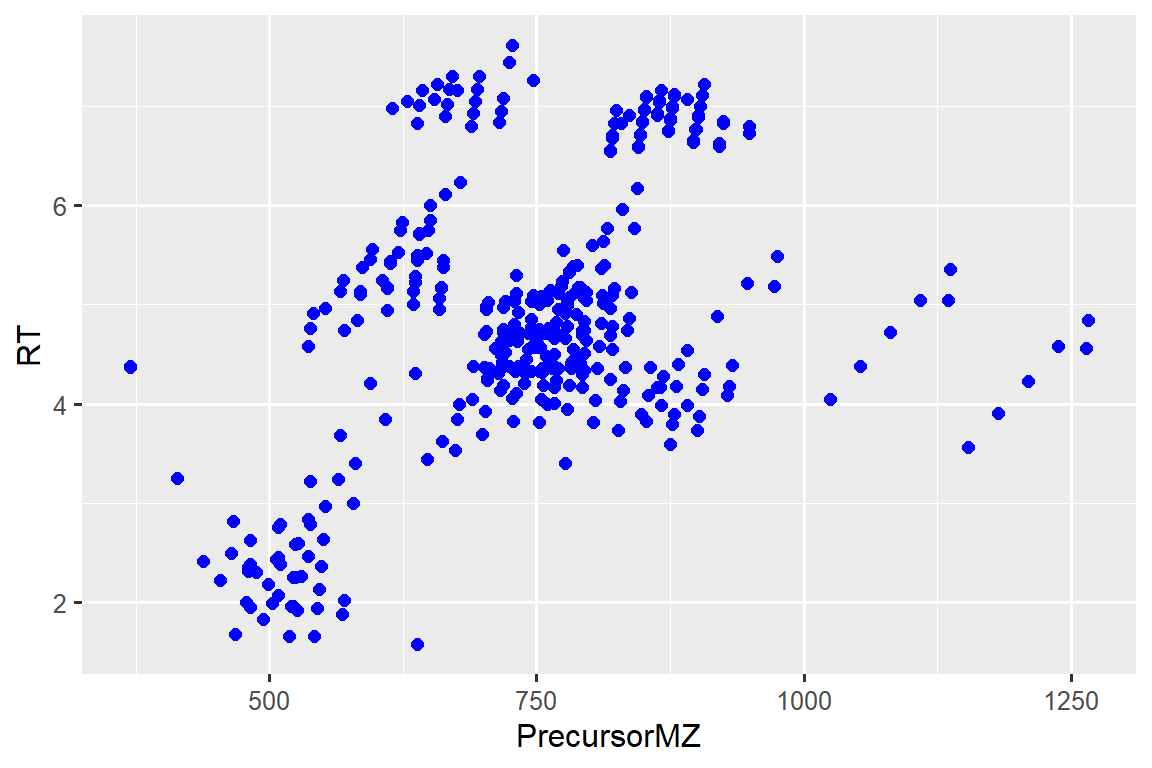
\includegraphics[width=18.75in,height=\textheight]{./datawrangling_files/figure-pdf/unnamed-chunk-4-2.pdf}

}

\end{figure}

\hypertarget{split-column-to-get-lipid-class}{%
\section{Split column to get lipid
class}\label{split-column-to-get-lipid-class}}

\begin{Shaded}
\begin{Highlighting}[]
\NormalTok{d\_plot\_wclass }\OtherTok{\textless{}{-}}\NormalTok{ d\_plot }\SpecialCharTok{|\textgreater{}} 
  \FunctionTok{separate}\NormalTok{(}
    \AttributeTok{col =}\NormalTok{ Compound,}
    \AttributeTok{into =} \FunctionTok{c}\NormalTok{(}\StringTok{"lipidclass"}\NormalTok{, }\StringTok{"chain"}\NormalTok{), }
    \AttributeTok{sep =} \StringTok{" "}\NormalTok{,}
    \AttributeTok{extra =} \StringTok{"merge"}\NormalTok{, }
    \AttributeTok{remove =} \ConstantTok{FALSE}\NormalTok{) }
    
\NormalTok{d\_plot\_wclass}
\end{Highlighting}
\end{Shaded}

\begin{verbatim}
#> # A tibble: 428 x 8
#>   AnalysisID      QCtype Compound lipidclass chain Intensity    RT PrecursorMZ
#>   <chr>           <chr>  <chr>    <chr>      <chr>     <dbl> <dbl>       <dbl>
#> 1 066_BQC_PQC07.d BQC    CE 14:0  CE         14:0       1152  6.98        615.
#> 2 066_BQC_PQC07.d BQC    CE 15:0  CE         15:0        984  7.06        629.
#> 3 066_BQC_PQC07.d BQC    CE 16:0  CE         16:0      93268  7.16        643.
#> 4 066_BQC_PQC07.d BQC    CE 16:1  CE         16:1      51054  7.01        641.
#> 5 066_BQC_PQC07.d BQC    CE 16:2  CE         16:2       1870  6.83        639.
#> 6 066_BQC_PQC07.d BQC    CE 17:0  CE         17:0       9050  7.22        657.
#> # ... with 422 more rows
\end{verbatim}

\hypertarget{now-lets-plot-again}{%
\section{Now let's plot again}\label{now-lets-plot-again}}

\begin{Shaded}
\begin{Highlighting}[]
\CommentTok{\# ggplot}
\FunctionTok{ggplot}\NormalTok{(d\_plot\_wclass, }\FunctionTok{aes}\NormalTok{(}\AttributeTok{x =}\NormalTok{ PrecursorMZ, }\AttributeTok{y =}\NormalTok{ RT, }\AttributeTok{color =}\NormalTok{ lipidclass)) }\SpecialCharTok{+}
  \FunctionTok{geom\_point}\NormalTok{(}\AttributeTok{size =} \DecValTok{2}\NormalTok{)}
\end{Highlighting}
\end{Shaded}

\begin{verbatim}
#> Warning: Removed 2 rows containing missing values (geom_point).
\end{verbatim}

\begin{figure}[H]

{\centering 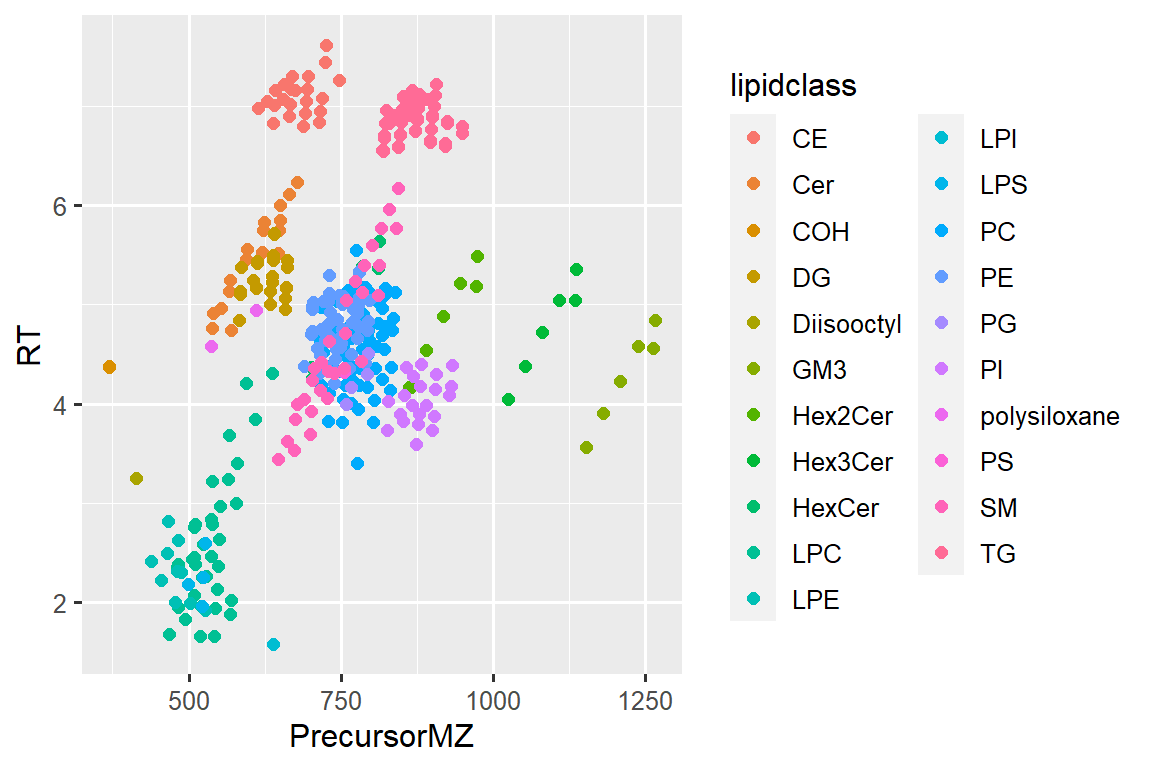
\includegraphics[width=18.75in,height=\textheight]{./datawrangling_files/figure-pdf/unnamed-chunk-5-1.pdf}

}

\end{figure}

\hypertarget{another-time}{%
\section{\ldots{} another time}\label{another-time}}

\begin{Shaded}
\begin{Highlighting}[]
\CommentTok{\# ggplot}
\FunctionTok{ggplot}\NormalTok{(d\_plot\_wclass, }\FunctionTok{aes}\NormalTok{(}\AttributeTok{x =}\NormalTok{ PrecursorMZ, }\AttributeTok{y =}\NormalTok{ RT, }\AttributeTok{color =}\NormalTok{ lipidclass, }\AttributeTok{size =}\NormalTok{ Intensity}\SpecialCharTok{/}\DecValTok{10}\NormalTok{)) }\SpecialCharTok{+}
  \FunctionTok{geom\_point}\NormalTok{()}
\end{Highlighting}
\end{Shaded}

\begin{verbatim}
#> Warning: Removed 2 rows containing missing values (geom_point).
\end{verbatim}

\begin{figure}[H]

{\centering 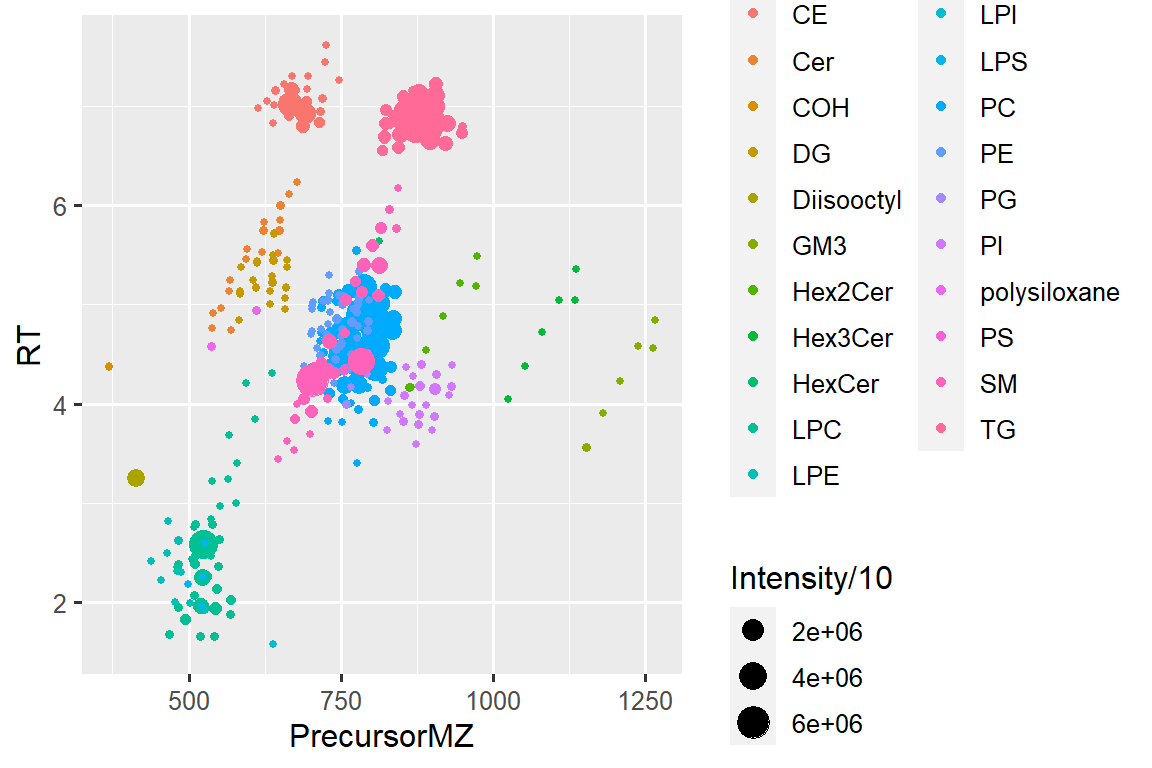
\includegraphics[width=18.75in,height=\textheight]{./datawrangling_files/figure-pdf/unnamed-chunk-6-1.pdf}

}

\end{figure}

\hypertarget{comparisons-in-r}{%
\section{Comparisons in R}\label{comparisons-in-r}}

Run following lines and try understand the result

\begin{Shaded}
\begin{Highlighting}[]
\StringTok{"CE 18:1"} \SpecialCharTok{==} \StringTok{"CE 18:1"}
\StringTok{"CE 18:1"} \SpecialCharTok{==} \StringTok{"CE 18:1 "}
\StringTok{"CE 18:1"} \SpecialCharTok{==} \StringTok{"CE  18:1"}
\StringTok{"Ce 18:1"} \SpecialCharTok{==} \StringTok{"CE 18:1"}

\NormalTok{stringr}\SpecialCharTok{::}\FunctionTok{str\_trim}\NormalTok{(}\StringTok{"CE 18:1 "}\NormalTok{)}
\NormalTok{stringr}\SpecialCharTok{::}\FunctionTok{str\_trim}\NormalTok{(}\StringTok{"   CE    18:1 "}\NormalTok{)}
\NormalTok{stringr}\SpecialCharTok{::}\FunctionTok{str\_squish}\NormalTok{(}\StringTok{"   CE    18:1 "}\NormalTok{)}

\NormalTok{stringr}\SpecialCharTok{::}\FunctionTok{str\_detect}\NormalTok{(}\StringTok{"LPC 18:1 (IS)"}\NormalTok{, }\AttributeTok{pattern =} \StringTok{"IS"}\NormalTok{)}
\NormalTok{stringr}\SpecialCharTok{::}\FunctionTok{str\_detect}\NormalTok{(}\StringTok{"LPC 18:1 (ISTD)"}\NormalTok{, }\AttributeTok{pattern =} \StringTok{"IS"}\NormalTok{)}
\NormalTok{stringr}\SpecialCharTok{::}\FunctionTok{str\_detect}\NormalTok{(}\StringTok{"LPC 18:1 (IS)"}\NormalTok{, }\AttributeTok{pattern =} \StringTok{"ISTD"}\NormalTok{)}
\NormalTok{stringr}\SpecialCharTok{::}\FunctionTok{str\_detect}\NormalTok{(}\StringTok{"LPC 18:1 (IS)"}\NormalTok{, }\AttributeTok{pattern =} \StringTok{"LPC"}\NormalTok{)}

\NormalTok{stringr}\SpecialCharTok{::}\FunctionTok{str\_replace}\NormalTok{(}\StringTok{"Acylcarnitine 18:1"}\NormalTok{, }
                     \AttributeTok{pattern =} \StringTok{"Acylcarnitine"}\NormalTok{,}
                     \AttributeTok{replacement =} \StringTok{"CAR"}\NormalTok{)}

\NormalTok{stringr}\SpecialCharTok{::}\FunctionTok{str\_replace}\NormalTok{(}\StringTok{"TG 48:2 [SIM] Results"}\NormalTok{, }
                     \AttributeTok{pattern =} \StringTok{" Results"}\NormalTok{,}
                     \AttributeTok{replacement =} \StringTok{""}\NormalTok{)}

\NormalTok{stringr}\SpecialCharTok{::}\FunctionTok{str\_replace}\NormalTok{(}\StringTok{"112\_BQC\_A9334.d"}\NormalTok{, }
                     \AttributeTok{pattern =} \StringTok{".d"}\NormalTok{,}
                     \AttributeTok{replacement =} \StringTok{""}\NormalTok{)}

\NormalTok{stringr}\SpecialCharTok{::}\FunctionTok{str\_to\_lower}\NormalTok{(}\StringTok{"CE 18:1"}\NormalTok{)}

\NormalTok{Sample\_ID }\OtherTok{\textless{}{-}} \DecValTok{1}
\FunctionTok{try}\NormalTok{(Sample}\SpecialCharTok{{-}}\NormalTok{ID }\OtherTok{\textless{}{-}} \DecValTok{1}\NormalTok{)}

\CommentTok{\# d |\textgreater{} filter(AnalysisID == "149\_BQC\_PQC17.d", }
\CommentTok{\#                    str\_detect(Compound, "IS|LPI") )}
\CommentTok{\# }
\CommentTok{\# d |\textgreater{} filter(str\_detect(AnalysisID, "BQC|TQC") , }
\CommentTok{\#                    str\_detect(Compound, "IS")) {-}\textgreater{} temp}
\end{Highlighting}
\end{Shaded}

\hypertarget{convert-long-table-to-wide-table-format}{%
\section{Convert long table to wide table
format}\label{convert-long-table-to-wide-table-format}}

\begin{Shaded}
\begin{Highlighting}[]
\CommentTok{\# d\_area\_temp \textless{}{-} d |\textgreater{} }
\CommentTok{\#   pivot\_wider(names\_from = "Compound" ,values\_from = "Area")}
\end{Highlighting}
\end{Shaded}

\begin{Shaded}
\begin{Highlighting}[]
\CommentTok{\# d\_BQC \textless{}{-} d\_area |\textgreater{} filter(QCtype == "BQC")}
\CommentTok{\# }
\CommentTok{\# }
\CommentTok{\# d\_res1 \textless{}{-} d\_BQC |\textgreater{}}
\CommentTok{\#   summarise(}
\CommentTok{\#     across(.cols = {-}seq\_no:{-}AcqTimeStamp,}
\CommentTok{\#            .fns = \textasciitilde{} sd(.)/mean(.)*100)}
\CommentTok{\#   )}
\CommentTok{\# d\_res1}
\CommentTok{\# }
\CommentTok{\# d\_BQC\_areas \textless{}{-} d\_BQC |\textgreater{} dplyr::select({-}seq\_no:{-}AcqTimeStamp)}

\CommentTok{\# d\_res2 \textless{}{-} purrr::map\_df(d\_BQC\_areas, .f = \textasciitilde{} sd(.)/mean(.)*100)}
\CommentTok{\# d\_res2}
\CommentTok{\# }
\CommentTok{\# d\_res3 \textless{}{-} sapply(X = d\_BQC\_areas, }
\CommentTok{\#                  FUN = function(x) c(CV = sd(x)/mean(x) * 100,}
\CommentTok{\#                                      RobustCV = mad(x)/median(x) * 100))}
\CommentTok{\# as.data.frame(d\_res3)}
\CommentTok{\# as.data.frame(t(d\_res3))}
\CommentTok{\# }
\CommentTok{\# d\_BQC\_long \textless{}{-} d\_BQC |\textgreater{} pivot\_longer(cols = {-}seq\_no:{-}AcqTimeStamp,}
\CommentTok{\#                                     names\_to = "Compound",}
\CommentTok{\#                                     values\_to = "Area")}
\CommentTok{\# }
\CommentTok{\# d\_BQC\_stats \textless{}{-} d\_BQC\_long |\textgreater{} }
\CommentTok{\#   group\_by(Compound) |\textgreater{} }
\CommentTok{\#   summarise(}
\CommentTok{\#     count = n(),}
\CommentTok{\#     Mean = mean(Area),}
\CommentTok{\#     Min = min(Area),}
\CommentTok{\#     CV = sd(Area)/mean(Area) *100,}
\CommentTok{\#     logCV = sqrt(exp(1)\^{}(sd(log(Area))\^{}2){-}1) *100,}
\CommentTok{\#     logCV\_roche = sqrt(10\^{}(log(10)*sd(log(Area, 10))\^{}2){-}1) *100,}
\CommentTok{\#     rCVq = 0.75 * IQR(Area, na.rm = TRUE)/median(Area) *100,}
\CommentTok{\#     rCVm = mad(Area, constant = 1.4826)/median(Area) *100}
\CommentTok{\#   )}
\CommentTok{\# d\_BQC\_stats}
\CommentTok{\# }
\CommentTok{\# hist(d\_BQC\_stats$CV)}
\CommentTok{\# hist(d\_BQC\_stats$rCVm)}
\CommentTok{\# }
\CommentTok{\# ggplot(d\_BQC\_stats) +}
\CommentTok{\#   geom\_histogram(aes(x=CV))}
\CommentTok{\# }
\CommentTok{\# d\_BQC\_stats\_long \textless{}{-} d\_BQC\_stats |\textgreater{}}
\CommentTok{\#   dplyr:::select(Compound, CV,rCVm,,rCVq, logCV) |\textgreater{} }
\CommentTok{\#   pivot\_longer(cols = {-}Compound, names\_to= "CV\_type" ,values\_to = "Value")}
\CommentTok{\# d\_BQC\_stats\_long}
\CommentTok{\# }
\CommentTok{\# ggplot(d\_BQC\_stats\_long) +}
\CommentTok{\#   geom\_histogram(aes(x=Value, fill = CV\_type)) + scale\_x\_continuous(limits = c(0,150)) + facet\_wrap(\textasciitilde{}CV\_type)}
\CommentTok{\# }
\CommentTok{\# }
\CommentTok{\# plot(d\_BQC\_stats$CV, d\_BQC\_stats$logCV)}
\CommentTok{\# plot(d\_BQC\_stats$CV, d\_BQC\_stats$logCV, xlim = c(0,100), ylim = c(0,100))}
\CommentTok{\# plot(d\_BQC\_stats$CV, d\_BQC\_stats$rCVm)}
\CommentTok{\# plot(d\_BQC\_stats$logCV, d\_BQC\_stats$rCVm, xlim = c(0,200))}
\CommentTok{\# plot(d\_BQC\_stats$CV, d\_BQC\_stats$rCVq)}
\end{Highlighting}
\end{Shaded}

\hypertarget{plotting-basics}{%
\chapter{Plotting Basics}\label{plotting-basics}}

We explore plotting using dilution series data as an example

\hypertarget{libraries}{%
\section{Libraries}\label{libraries}}

The package \texttt{ggpmisc} will only be used once in this chapter. It
provides additional functions for the annotating and plotting of fitted
models

\begin{Shaded}
\begin{Highlighting}[]
\FunctionTok{library}\NormalTok{(here)}
\FunctionTok{library}\NormalTok{(tidyverse)}
\FunctionTok{library}\NormalTok{(ggpmisc)}
\end{Highlighting}
\end{Shaded}

\hypertarget{import-datasets}{%
\section{Import Datasets}\label{import-datasets}}

We import a lipidomics dataset in a flat table with additinal columns
indicating QC types, injection volumes, and dilution series number

\begin{Shaded}
\begin{Highlighting}[]
\NormalTok{d\_orig }\OtherTok{\textless{}{-}} \FunctionTok{read\_csv}\NormalTok{(}\FunctionTok{here}\NormalTok{(}\StringTok{"data/Testdata\_Lipidomics\_flat\_wide\_annotated\_V1.csv"}\NormalTok{))}
\end{Highlighting}
\end{Shaded}

\begin{table}

\caption{\textbf{?(caption)}}\begin{minipage}[t]{\linewidth}

{\centering 

\begin{longtable}[]{@{}
  >{\raggedright\arraybackslash}p{(\columnwidth - 854\tabcolsep) * \real{0.0037}}
  >{\raggedright\arraybackslash}p{(\columnwidth - 854\tabcolsep) * \real{0.0012}}
  >{\raggedleft\arraybackslash}p{(\columnwidth - 854\tabcolsep) * \real{0.0014}}
  >{\raggedleft\arraybackslash}p{(\columnwidth - 854\tabcolsep) * \real{0.0012}}
  >{\raggedleft\arraybackslash}p{(\columnwidth - 854\tabcolsep) * \real{0.0014}}
  >{\raggedleft\arraybackslash}p{(\columnwidth - 854\tabcolsep) * \real{0.0014}}
  >{\raggedleft\arraybackslash}p{(\columnwidth - 854\tabcolsep) * \real{0.0014}}
  >{\raggedleft\arraybackslash}p{(\columnwidth - 854\tabcolsep) * \real{0.0014}}
  >{\raggedleft\arraybackslash}p{(\columnwidth - 854\tabcolsep) * \real{0.0014}}
  >{\raggedleft\arraybackslash}p{(\columnwidth - 854\tabcolsep) * \real{0.0014}}
  >{\raggedleft\arraybackslash}p{(\columnwidth - 854\tabcolsep) * \real{0.0014}}
  >{\raggedleft\arraybackslash}p{(\columnwidth - 854\tabcolsep) * \real{0.0032}}
  >{\raggedleft\arraybackslash}p{(\columnwidth - 854\tabcolsep) * \real{0.0016}}
  >{\raggedleft\arraybackslash}p{(\columnwidth - 854\tabcolsep) * \real{0.0014}}
  >{\raggedleft\arraybackslash}p{(\columnwidth - 854\tabcolsep) * \real{0.0014}}
  >{\raggedleft\arraybackslash}p{(\columnwidth - 854\tabcolsep) * \real{0.0014}}
  >{\raggedleft\arraybackslash}p{(\columnwidth - 854\tabcolsep) * \real{0.0014}}
  >{\raggedleft\arraybackslash}p{(\columnwidth - 854\tabcolsep) * \real{0.0016}}
  >{\raggedleft\arraybackslash}p{(\columnwidth - 854\tabcolsep) * \real{0.0014}}
  >{\raggedleft\arraybackslash}p{(\columnwidth - 854\tabcolsep) * \real{0.0014}}
  >{\raggedleft\arraybackslash}p{(\columnwidth - 854\tabcolsep) * \real{0.0014}}
  >{\raggedleft\arraybackslash}p{(\columnwidth - 854\tabcolsep) * \real{0.0014}}
  >{\raggedleft\arraybackslash}p{(\columnwidth - 854\tabcolsep) * \real{0.0014}}
  >{\raggedleft\arraybackslash}p{(\columnwidth - 854\tabcolsep) * \real{0.0014}}
  >{\raggedleft\arraybackslash}p{(\columnwidth - 854\tabcolsep) * \real{0.0014}}
  >{\raggedleft\arraybackslash}p{(\columnwidth - 854\tabcolsep) * \real{0.0027}}
  >{\raggedleft\arraybackslash}p{(\columnwidth - 854\tabcolsep) * \real{0.0027}}
  >{\raggedleft\arraybackslash}p{(\columnwidth - 854\tabcolsep) * \real{0.0027}}
  >{\raggedleft\arraybackslash}p{(\columnwidth - 854\tabcolsep) * \real{0.0027}}
  >{\raggedleft\arraybackslash}p{(\columnwidth - 854\tabcolsep) * \real{0.0037}}
  >{\raggedleft\arraybackslash}p{(\columnwidth - 854\tabcolsep) * \real{0.0027}}
  >{\raggedleft\arraybackslash}p{(\columnwidth - 854\tabcolsep) * \real{0.0037}}
  >{\raggedleft\arraybackslash}p{(\columnwidth - 854\tabcolsep) * \real{0.0027}}
  >{\raggedleft\arraybackslash}p{(\columnwidth - 854\tabcolsep) * \real{0.0046}}
  >{\raggedleft\arraybackslash}p{(\columnwidth - 854\tabcolsep) * \real{0.0027}}
  >{\raggedleft\arraybackslash}p{(\columnwidth - 854\tabcolsep) * \real{0.0027}}
  >{\raggedleft\arraybackslash}p{(\columnwidth - 854\tabcolsep) * \real{0.0027}}
  >{\raggedleft\arraybackslash}p{(\columnwidth - 854\tabcolsep) * \real{0.0027}}
  >{\raggedleft\arraybackslash}p{(\columnwidth - 854\tabcolsep) * \real{0.0027}}
  >{\raggedleft\arraybackslash}p{(\columnwidth - 854\tabcolsep) * \real{0.0027}}
  >{\raggedleft\arraybackslash}p{(\columnwidth - 854\tabcolsep) * \real{0.0027}}
  >{\raggedleft\arraybackslash}p{(\columnwidth - 854\tabcolsep) * \real{0.0027}}
  >{\raggedleft\arraybackslash}p{(\columnwidth - 854\tabcolsep) * \real{0.0027}}
  >{\raggedleft\arraybackslash}p{(\columnwidth - 854\tabcolsep) * \real{0.0027}}
  >{\raggedleft\arraybackslash}p{(\columnwidth - 854\tabcolsep) * \real{0.0018}}
  >{\raggedleft\arraybackslash}p{(\columnwidth - 854\tabcolsep) * \real{0.0016}}
  >{\raggedleft\arraybackslash}p{(\columnwidth - 854\tabcolsep) * \real{0.0037}}
  >{\raggedleft\arraybackslash}p{(\columnwidth - 854\tabcolsep) * \real{0.0037}}
  >{\raggedleft\arraybackslash}p{(\columnwidth - 854\tabcolsep) * \real{0.0037}}
  >{\raggedleft\arraybackslash}p{(\columnwidth - 854\tabcolsep) * \real{0.0037}}
  >{\raggedleft\arraybackslash}p{(\columnwidth - 854\tabcolsep) * \real{0.0055}}
  >{\raggedleft\arraybackslash}p{(\columnwidth - 854\tabcolsep) * \real{0.0055}}
  >{\raggedleft\arraybackslash}p{(\columnwidth - 854\tabcolsep) * \real{0.0037}}
  >{\raggedleft\arraybackslash}p{(\columnwidth - 854\tabcolsep) * \real{0.0037}}
  >{\raggedleft\arraybackslash}p{(\columnwidth - 854\tabcolsep) * \real{0.0037}}
  >{\raggedleft\arraybackslash}p{(\columnwidth - 854\tabcolsep) * \real{0.0037}}
  >{\raggedleft\arraybackslash}p{(\columnwidth - 854\tabcolsep) * \real{0.0037}}
  >{\raggedleft\arraybackslash}p{(\columnwidth - 854\tabcolsep) * \real{0.0037}}
  >{\raggedleft\arraybackslash}p{(\columnwidth - 854\tabcolsep) * \real{0.0037}}
  >{\raggedleft\arraybackslash}p{(\columnwidth - 854\tabcolsep) * \real{0.0037}}
  >{\raggedleft\arraybackslash}p{(\columnwidth - 854\tabcolsep) * \real{0.0037}}
  >{\raggedleft\arraybackslash}p{(\columnwidth - 854\tabcolsep) * \real{0.0037}}
  >{\raggedleft\arraybackslash}p{(\columnwidth - 854\tabcolsep) * \real{0.0037}}
  >{\raggedleft\arraybackslash}p{(\columnwidth - 854\tabcolsep) * \real{0.0037}}
  >{\raggedleft\arraybackslash}p{(\columnwidth - 854\tabcolsep) * \real{0.0037}}
  >{\raggedleft\arraybackslash}p{(\columnwidth - 854\tabcolsep) * \real{0.0037}}
  >{\raggedleft\arraybackslash}p{(\columnwidth - 854\tabcolsep) * \real{0.0037}}
  >{\raggedleft\arraybackslash}p{(\columnwidth - 854\tabcolsep) * \real{0.0037}}
  >{\raggedleft\arraybackslash}p{(\columnwidth - 854\tabcolsep) * \real{0.0037}}
  >{\raggedleft\arraybackslash}p{(\columnwidth - 854\tabcolsep) * \real{0.0037}}
  >{\raggedleft\arraybackslash}p{(\columnwidth - 854\tabcolsep) * \real{0.0037}}
  >{\raggedleft\arraybackslash}p{(\columnwidth - 854\tabcolsep) * \real{0.0037}}
  >{\raggedleft\arraybackslash}p{(\columnwidth - 854\tabcolsep) * \real{0.0037}}
  >{\raggedleft\arraybackslash}p{(\columnwidth - 854\tabcolsep) * \real{0.0037}}
  >{\raggedleft\arraybackslash}p{(\columnwidth - 854\tabcolsep) * \real{0.0037}}
  >{\raggedleft\arraybackslash}p{(\columnwidth - 854\tabcolsep) * \real{0.0037}}
  >{\raggedleft\arraybackslash}p{(\columnwidth - 854\tabcolsep) * \real{0.0037}}
  >{\raggedleft\arraybackslash}p{(\columnwidth - 854\tabcolsep) * \real{0.0037}}
  >{\raggedleft\arraybackslash}p{(\columnwidth - 854\tabcolsep) * \real{0.0037}}
  >{\raggedleft\arraybackslash}p{(\columnwidth - 854\tabcolsep) * \real{0.0037}}
  >{\raggedleft\arraybackslash}p{(\columnwidth - 854\tabcolsep) * \real{0.0037}}
  >{\raggedleft\arraybackslash}p{(\columnwidth - 854\tabcolsep) * \real{0.0027}}
  >{\raggedleft\arraybackslash}p{(\columnwidth - 854\tabcolsep) * \real{0.0027}}
  >{\raggedleft\arraybackslash}p{(\columnwidth - 854\tabcolsep) * \real{0.0027}}
  >{\raggedleft\arraybackslash}p{(\columnwidth - 854\tabcolsep) * \real{0.0027}}
  >{\raggedleft\arraybackslash}p{(\columnwidth - 854\tabcolsep) * \real{0.0027}}
  >{\raggedleft\arraybackslash}p{(\columnwidth - 854\tabcolsep) * \real{0.0027}}
  >{\raggedleft\arraybackslash}p{(\columnwidth - 854\tabcolsep) * \real{0.0034}}
  >{\raggedleft\arraybackslash}p{(\columnwidth - 854\tabcolsep) * \real{0.0051}}
  >{\raggedleft\arraybackslash}p{(\columnwidth - 854\tabcolsep) * \real{0.0034}}
  >{\raggedleft\arraybackslash}p{(\columnwidth - 854\tabcolsep) * \real{0.0034}}
  >{\raggedleft\arraybackslash}p{(\columnwidth - 854\tabcolsep) * \real{0.0034}}
  >{\raggedleft\arraybackslash}p{(\columnwidth - 854\tabcolsep) * \real{0.0034}}
  >{\raggedleft\arraybackslash}p{(\columnwidth - 854\tabcolsep) * \real{0.0034}}
  >{\raggedleft\arraybackslash}p{(\columnwidth - 854\tabcolsep) * \real{0.0034}}
  >{\raggedleft\arraybackslash}p{(\columnwidth - 854\tabcolsep) * \real{0.0034}}
  >{\raggedleft\arraybackslash}p{(\columnwidth - 854\tabcolsep) * \real{0.0034}}
  >{\raggedleft\arraybackslash}p{(\columnwidth - 854\tabcolsep) * \real{0.0034}}
  >{\raggedleft\arraybackslash}p{(\columnwidth - 854\tabcolsep) * \real{0.0034}}
  >{\raggedleft\arraybackslash}p{(\columnwidth - 854\tabcolsep) * \real{0.0034}}
  >{\raggedleft\arraybackslash}p{(\columnwidth - 854\tabcolsep) * \real{0.0032}}
  >{\raggedleft\arraybackslash}p{(\columnwidth - 854\tabcolsep) * \real{0.0049}}
  >{\raggedleft\arraybackslash}p{(\columnwidth - 854\tabcolsep) * \real{0.0032}}
  >{\raggedleft\arraybackslash}p{(\columnwidth - 854\tabcolsep) * \real{0.0032}}
  >{\raggedleft\arraybackslash}p{(\columnwidth - 854\tabcolsep) * \real{0.0032}}
  >{\raggedleft\arraybackslash}p{(\columnwidth - 854\tabcolsep) * \real{0.0032}}
  >{\raggedleft\arraybackslash}p{(\columnwidth - 854\tabcolsep) * \real{0.0032}}
  >{\raggedleft\arraybackslash}p{(\columnwidth - 854\tabcolsep) * \real{0.0016}}
  >{\raggedleft\arraybackslash}p{(\columnwidth - 854\tabcolsep) * \real{0.0016}}
  >{\raggedleft\arraybackslash}p{(\columnwidth - 854\tabcolsep) * \real{0.0016}}
  >{\raggedleft\arraybackslash}p{(\columnwidth - 854\tabcolsep) * \real{0.0016}}
  >{\raggedleft\arraybackslash}p{(\columnwidth - 854\tabcolsep) * \real{0.0016}}
  >{\raggedleft\arraybackslash}p{(\columnwidth - 854\tabcolsep) * \real{0.0016}}
  >{\raggedleft\arraybackslash}p{(\columnwidth - 854\tabcolsep) * \real{0.0016}}
  >{\raggedleft\arraybackslash}p{(\columnwidth - 854\tabcolsep) * \real{0.0034}}
  >{\raggedleft\arraybackslash}p{(\columnwidth - 854\tabcolsep) * \real{0.0016}}
  >{\raggedleft\arraybackslash}p{(\columnwidth - 854\tabcolsep) * \real{0.0016}}
  >{\raggedleft\arraybackslash}p{(\columnwidth - 854\tabcolsep) * \real{0.0016}}
  >{\raggedleft\arraybackslash}p{(\columnwidth - 854\tabcolsep) * \real{0.0016}}
  >{\raggedleft\arraybackslash}p{(\columnwidth - 854\tabcolsep) * \real{0.0016}}
  >{\raggedleft\arraybackslash}p{(\columnwidth - 854\tabcolsep) * \real{0.0016}}
  >{\raggedleft\arraybackslash}p{(\columnwidth - 854\tabcolsep) * \real{0.0016}}
  >{\raggedleft\arraybackslash}p{(\columnwidth - 854\tabcolsep) * \real{0.0016}}
  >{\raggedleft\arraybackslash}p{(\columnwidth - 854\tabcolsep) * \real{0.0016}}
  >{\raggedleft\arraybackslash}p{(\columnwidth - 854\tabcolsep) * \real{0.0016}}
  >{\raggedleft\arraybackslash}p{(\columnwidth - 854\tabcolsep) * \real{0.0016}}
  >{\raggedleft\arraybackslash}p{(\columnwidth - 854\tabcolsep) * \real{0.0016}}
  >{\raggedleft\arraybackslash}p{(\columnwidth - 854\tabcolsep) * \real{0.0016}}
  >{\raggedleft\arraybackslash}p{(\columnwidth - 854\tabcolsep) * \real{0.0016}}
  >{\raggedleft\arraybackslash}p{(\columnwidth - 854\tabcolsep) * \real{0.0016}}
  >{\raggedleft\arraybackslash}p{(\columnwidth - 854\tabcolsep) * \real{0.0016}}
  >{\raggedleft\arraybackslash}p{(\columnwidth - 854\tabcolsep) * \real{0.0019}}
  >{\raggedleft\arraybackslash}p{(\columnwidth - 854\tabcolsep) * \real{0.0019}}
  >{\raggedleft\arraybackslash}p{(\columnwidth - 854\tabcolsep) * \real{0.0019}}
  >{\raggedleft\arraybackslash}p{(\columnwidth - 854\tabcolsep) * \real{0.0019}}
  >{\raggedleft\arraybackslash}p{(\columnwidth - 854\tabcolsep) * \real{0.0019}}
  >{\raggedleft\arraybackslash}p{(\columnwidth - 854\tabcolsep) * \real{0.0019}}
  >{\raggedleft\arraybackslash}p{(\columnwidth - 854\tabcolsep) * \real{0.0019}}
  >{\raggedleft\arraybackslash}p{(\columnwidth - 854\tabcolsep) * \real{0.0019}}
  >{\raggedleft\arraybackslash}p{(\columnwidth - 854\tabcolsep) * \real{0.0019}}
  >{\raggedleft\arraybackslash}p{(\columnwidth - 854\tabcolsep) * \real{0.0019}}
  >{\raggedleft\arraybackslash}p{(\columnwidth - 854\tabcolsep) * \real{0.0019}}
  >{\raggedleft\arraybackslash}p{(\columnwidth - 854\tabcolsep) * \real{0.0019}}
  >{\raggedleft\arraybackslash}p{(\columnwidth - 854\tabcolsep) * \real{0.0016}}
  >{\raggedleft\arraybackslash}p{(\columnwidth - 854\tabcolsep) * \real{0.0016}}
  >{\raggedleft\arraybackslash}p{(\columnwidth - 854\tabcolsep) * \real{0.0016}}
  >{\raggedleft\arraybackslash}p{(\columnwidth - 854\tabcolsep) * \real{0.0034}}
  >{\raggedleft\arraybackslash}p{(\columnwidth - 854\tabcolsep) * \real{0.0016}}
  >{\raggedleft\arraybackslash}p{(\columnwidth - 854\tabcolsep) * \real{0.0016}}
  >{\raggedleft\arraybackslash}p{(\columnwidth - 854\tabcolsep) * \real{0.0016}}
  >{\raggedleft\arraybackslash}p{(\columnwidth - 854\tabcolsep) * \real{0.0019}}
  >{\raggedleft\arraybackslash}p{(\columnwidth - 854\tabcolsep) * \real{0.0019}}
  >{\raggedleft\arraybackslash}p{(\columnwidth - 854\tabcolsep) * \real{0.0019}}
  >{\raggedleft\arraybackslash}p{(\columnwidth - 854\tabcolsep) * \real{0.0016}}
  >{\raggedleft\arraybackslash}p{(\columnwidth - 854\tabcolsep) * \real{0.0016}}
  >{\raggedleft\arraybackslash}p{(\columnwidth - 854\tabcolsep) * \real{0.0016}}
  >{\raggedleft\arraybackslash}p{(\columnwidth - 854\tabcolsep) * \real{0.0016}}
  >{\raggedleft\arraybackslash}p{(\columnwidth - 854\tabcolsep) * \real{0.0016}}
  >{\raggedleft\arraybackslash}p{(\columnwidth - 854\tabcolsep) * \real{0.0014}}
  >{\raggedleft\arraybackslash}p{(\columnwidth - 854\tabcolsep) * \real{0.0014}}
  >{\raggedleft\arraybackslash}p{(\columnwidth - 854\tabcolsep) * \real{0.0014}}
  >{\raggedleft\arraybackslash}p{(\columnwidth - 854\tabcolsep) * \real{0.0014}}
  >{\raggedleft\arraybackslash}p{(\columnwidth - 854\tabcolsep) * \real{0.0014}}
  >{\raggedleft\arraybackslash}p{(\columnwidth - 854\tabcolsep) * \real{0.0014}}
  >{\raggedleft\arraybackslash}p{(\columnwidth - 854\tabcolsep) * \real{0.0014}}
  >{\raggedleft\arraybackslash}p{(\columnwidth - 854\tabcolsep) * \real{0.0032}}
  >{\raggedleft\arraybackslash}p{(\columnwidth - 854\tabcolsep) * \real{0.0014}}
  >{\raggedleft\arraybackslash}p{(\columnwidth - 854\tabcolsep) * \real{0.0014}}
  >{\raggedleft\arraybackslash}p{(\columnwidth - 854\tabcolsep) * \real{0.0016}}
  >{\raggedleft\arraybackslash}p{(\columnwidth - 854\tabcolsep) * \real{0.0016}}
  >{\raggedleft\arraybackslash}p{(\columnwidth - 854\tabcolsep) * \real{0.0023}}
  >{\raggedleft\arraybackslash}p{(\columnwidth - 854\tabcolsep) * \real{0.0071}}
  >{\raggedleft\arraybackslash}p{(\columnwidth - 854\tabcolsep) * \real{0.0014}}
  >{\raggedleft\arraybackslash}p{(\columnwidth - 854\tabcolsep) * \real{0.0014}}
  >{\raggedleft\arraybackslash}p{(\columnwidth - 854\tabcolsep) * \real{0.0014}}
  >{\raggedleft\arraybackslash}p{(\columnwidth - 854\tabcolsep) * \real{0.0014}}
  >{\raggedleft\arraybackslash}p{(\columnwidth - 854\tabcolsep) * \real{0.0014}}
  >{\raggedleft\arraybackslash}p{(\columnwidth - 854\tabcolsep) * \real{0.0014}}
  >{\raggedleft\arraybackslash}p{(\columnwidth - 854\tabcolsep) * \real{0.0014}}
  >{\raggedleft\arraybackslash}p{(\columnwidth - 854\tabcolsep) * \real{0.0014}}
  >{\raggedleft\arraybackslash}p{(\columnwidth - 854\tabcolsep) * \real{0.0016}}
  >{\raggedleft\arraybackslash}p{(\columnwidth - 854\tabcolsep) * \real{0.0016}}
  >{\raggedleft\arraybackslash}p{(\columnwidth - 854\tabcolsep) * \real{0.0016}}
  >{\raggedleft\arraybackslash}p{(\columnwidth - 854\tabcolsep) * \real{0.0018}}
  >{\raggedleft\arraybackslash}p{(\columnwidth - 854\tabcolsep) * \real{0.0018}}
  >{\raggedleft\arraybackslash}p{(\columnwidth - 854\tabcolsep) * \real{0.0014}}
  >{\raggedleft\arraybackslash}p{(\columnwidth - 854\tabcolsep) * \real{0.0014}}
  >{\raggedleft\arraybackslash}p{(\columnwidth - 854\tabcolsep) * \real{0.0014}}
  >{\raggedleft\arraybackslash}p{(\columnwidth - 854\tabcolsep) * \real{0.0014}}
  >{\raggedleft\arraybackslash}p{(\columnwidth - 854\tabcolsep) * \real{0.0014}}
  >{\raggedleft\arraybackslash}p{(\columnwidth - 854\tabcolsep) * \real{0.0014}}
  >{\raggedleft\arraybackslash}p{(\columnwidth - 854\tabcolsep) * \real{0.0016}}
  >{\raggedleft\arraybackslash}p{(\columnwidth - 854\tabcolsep) * \real{0.0016}}
  >{\raggedleft\arraybackslash}p{(\columnwidth - 854\tabcolsep) * \real{0.0048}}
  >{\raggedleft\arraybackslash}p{(\columnwidth - 854\tabcolsep) * \real{0.0016}}
  >{\raggedleft\arraybackslash}p{(\columnwidth - 854\tabcolsep) * \real{0.0014}}
  >{\raggedleft\arraybackslash}p{(\columnwidth - 854\tabcolsep) * \real{0.0014}}
  >{\raggedleft\arraybackslash}p{(\columnwidth - 854\tabcolsep) * \real{0.0014}}
  >{\raggedleft\arraybackslash}p{(\columnwidth - 854\tabcolsep) * \real{0.0014}}
  >{\raggedleft\arraybackslash}p{(\columnwidth - 854\tabcolsep) * \real{0.0014}}
  >{\raggedleft\arraybackslash}p{(\columnwidth - 854\tabcolsep) * \real{0.0081}}
  >{\raggedleft\arraybackslash}p{(\columnwidth - 854\tabcolsep) * \real{0.0048}}
  >{\raggedleft\arraybackslash}p{(\columnwidth - 854\tabcolsep) * \real{0.0016}}
  >{\raggedleft\arraybackslash}p{(\columnwidth - 854\tabcolsep) * \real{0.0014}}
  >{\raggedleft\arraybackslash}p{(\columnwidth - 854\tabcolsep) * \real{0.0014}}
  >{\raggedleft\arraybackslash}p{(\columnwidth - 854\tabcolsep) * \real{0.0018}}
  >{\raggedleft\arraybackslash}p{(\columnwidth - 854\tabcolsep) * \real{0.0018}}
  >{\raggedleft\arraybackslash}p{(\columnwidth - 854\tabcolsep) * \real{0.0018}}
  >{\raggedleft\arraybackslash}p{(\columnwidth - 854\tabcolsep) * \real{0.0018}}
  >{\raggedleft\arraybackslash}p{(\columnwidth - 854\tabcolsep) * \real{0.0018}}
  >{\raggedleft\arraybackslash}p{(\columnwidth - 854\tabcolsep) * \real{0.0018}}
  >{\raggedleft\arraybackslash}p{(\columnwidth - 854\tabcolsep) * \real{0.0018}}
  >{\raggedleft\arraybackslash}p{(\columnwidth - 854\tabcolsep) * \real{0.0018}}
  >{\raggedleft\arraybackslash}p{(\columnwidth - 854\tabcolsep) * \real{0.0018}}
  >{\raggedleft\arraybackslash}p{(\columnwidth - 854\tabcolsep) * \real{0.0018}}
  >{\raggedleft\arraybackslash}p{(\columnwidth - 854\tabcolsep) * \real{0.0018}}
  >{\raggedleft\arraybackslash}p{(\columnwidth - 854\tabcolsep) * \real{0.0018}}
  >{\raggedleft\arraybackslash}p{(\columnwidth - 854\tabcolsep) * \real{0.0018}}
  >{\raggedleft\arraybackslash}p{(\columnwidth - 854\tabcolsep) * \real{0.0018}}
  >{\raggedleft\arraybackslash}p{(\columnwidth - 854\tabcolsep) * \real{0.0018}}
  >{\raggedleft\arraybackslash}p{(\columnwidth - 854\tabcolsep) * \real{0.0018}}
  >{\raggedleft\arraybackslash}p{(\columnwidth - 854\tabcolsep) * \real{0.0018}}
  >{\raggedleft\arraybackslash}p{(\columnwidth - 854\tabcolsep) * \real{0.0018}}
  >{\raggedleft\arraybackslash}p{(\columnwidth - 854\tabcolsep) * \real{0.0018}}
  >{\raggedleft\arraybackslash}p{(\columnwidth - 854\tabcolsep) * \real{0.0018}}
  >{\raggedleft\arraybackslash}p{(\columnwidth - 854\tabcolsep) * \real{0.0018}}
  >{\raggedleft\arraybackslash}p{(\columnwidth - 854\tabcolsep) * \real{0.0018}}
  >{\raggedleft\arraybackslash}p{(\columnwidth - 854\tabcolsep) * \real{0.0018}}
  >{\raggedleft\arraybackslash}p{(\columnwidth - 854\tabcolsep) * \real{0.0018}}
  >{\raggedleft\arraybackslash}p{(\columnwidth - 854\tabcolsep) * \real{0.0018}}
  >{\raggedleft\arraybackslash}p{(\columnwidth - 854\tabcolsep) * \real{0.0018}}
  >{\raggedleft\arraybackslash}p{(\columnwidth - 854\tabcolsep) * \real{0.0018}}
  >{\raggedleft\arraybackslash}p{(\columnwidth - 854\tabcolsep) * \real{0.0018}}
  >{\raggedleft\arraybackslash}p{(\columnwidth - 854\tabcolsep) * \real{0.0014}}
  >{\raggedleft\arraybackslash}p{(\columnwidth - 854\tabcolsep) * \real{0.0032}}
  >{\raggedleft\arraybackslash}p{(\columnwidth - 854\tabcolsep) * \real{0.0014}}
  >{\raggedleft\arraybackslash}p{(\columnwidth - 854\tabcolsep) * \real{0.0014}}
  >{\raggedleft\arraybackslash}p{(\columnwidth - 854\tabcolsep) * \real{0.0014}}
  >{\raggedleft\arraybackslash}p{(\columnwidth - 854\tabcolsep) * \real{0.0014}}
  >{\raggedleft\arraybackslash}p{(\columnwidth - 854\tabcolsep) * \real{0.0014}}
  >{\raggedleft\arraybackslash}p{(\columnwidth - 854\tabcolsep) * \real{0.0014}}
  >{\raggedleft\arraybackslash}p{(\columnwidth - 854\tabcolsep) * \real{0.0014}}
  >{\raggedleft\arraybackslash}p{(\columnwidth - 854\tabcolsep) * \real{0.0014}}
  >{\raggedleft\arraybackslash}p{(\columnwidth - 854\tabcolsep) * \real{0.0048}}
  >{\raggedleft\arraybackslash}p{(\columnwidth - 854\tabcolsep) * \real{0.0018}}
  >{\raggedleft\arraybackslash}p{(\columnwidth - 854\tabcolsep) * \real{0.0018}}
  >{\raggedleft\arraybackslash}p{(\columnwidth - 854\tabcolsep) * \real{0.0014}}
  >{\raggedleft\arraybackslash}p{(\columnwidth - 854\tabcolsep) * \real{0.0014}}
  >{\raggedleft\arraybackslash}p{(\columnwidth - 854\tabcolsep) * \real{0.0014}}
  >{\raggedleft\arraybackslash}p{(\columnwidth - 854\tabcolsep) * \real{0.0014}}
  >{\raggedleft\arraybackslash}p{(\columnwidth - 854\tabcolsep) * \real{0.0014}}
  >{\raggedleft\arraybackslash}p{(\columnwidth - 854\tabcolsep) * \real{0.0014}}
  >{\raggedleft\arraybackslash}p{(\columnwidth - 854\tabcolsep) * \real{0.0014}}
  >{\raggedleft\arraybackslash}p{(\columnwidth - 854\tabcolsep) * \real{0.0048}}
  >{\raggedleft\arraybackslash}p{(\columnwidth - 854\tabcolsep) * \real{0.0014}}
  >{\raggedleft\arraybackslash}p{(\columnwidth - 854\tabcolsep) * \real{0.0014}}
  >{\raggedleft\arraybackslash}p{(\columnwidth - 854\tabcolsep) * \real{0.0018}}
  >{\raggedleft\arraybackslash}p{(\columnwidth - 854\tabcolsep) * \real{0.0018}}
  >{\raggedleft\arraybackslash}p{(\columnwidth - 854\tabcolsep) * \real{0.0018}}
  >{\raggedleft\arraybackslash}p{(\columnwidth - 854\tabcolsep) * \real{0.0018}}
  >{\raggedleft\arraybackslash}p{(\columnwidth - 854\tabcolsep) * \real{0.0018}}
  >{\raggedleft\arraybackslash}p{(\columnwidth - 854\tabcolsep) * \real{0.0018}}
  >{\raggedleft\arraybackslash}p{(\columnwidth - 854\tabcolsep) * \real{0.0018}}
  >{\raggedleft\arraybackslash}p{(\columnwidth - 854\tabcolsep) * \real{0.0018}}
  >{\raggedleft\arraybackslash}p{(\columnwidth - 854\tabcolsep) * \real{0.0018}}
  >{\raggedleft\arraybackslash}p{(\columnwidth - 854\tabcolsep) * \real{0.0018}}
  >{\raggedleft\arraybackslash}p{(\columnwidth - 854\tabcolsep) * \real{0.0035}}
  >{\raggedleft\arraybackslash}p{(\columnwidth - 854\tabcolsep) * \real{0.0049}}
  >{\raggedleft\arraybackslash}p{(\columnwidth - 854\tabcolsep) * \real{0.0035}}
  >{\raggedleft\arraybackslash}p{(\columnwidth - 854\tabcolsep) * \real{0.0049}}
  >{\raggedleft\arraybackslash}p{(\columnwidth - 854\tabcolsep) * \real{0.0035}}
  >{\raggedleft\arraybackslash}p{(\columnwidth - 854\tabcolsep) * \real{0.0049}}
  >{\raggedleft\arraybackslash}p{(\columnwidth - 854\tabcolsep) * \real{0.0035}}
  >{\raggedleft\arraybackslash}p{(\columnwidth - 854\tabcolsep) * \real{0.0049}}
  >{\raggedleft\arraybackslash}p{(\columnwidth - 854\tabcolsep) * \real{0.0035}}
  >{\raggedleft\arraybackslash}p{(\columnwidth - 854\tabcolsep) * \real{0.0049}}
  >{\raggedleft\arraybackslash}p{(\columnwidth - 854\tabcolsep) * \real{0.0035}}
  >{\raggedleft\arraybackslash}p{(\columnwidth - 854\tabcolsep) * \real{0.0049}}
  >{\raggedleft\arraybackslash}p{(\columnwidth - 854\tabcolsep) * \real{0.0035}}
  >{\raggedleft\arraybackslash}p{(\columnwidth - 854\tabcolsep) * \real{0.0049}}
  >{\raggedleft\arraybackslash}p{(\columnwidth - 854\tabcolsep) * \real{0.0035}}
  >{\raggedleft\arraybackslash}p{(\columnwidth - 854\tabcolsep) * \real{0.0049}}
  >{\raggedleft\arraybackslash}p{(\columnwidth - 854\tabcolsep) * \real{0.0035}}
  >{\raggedleft\arraybackslash}p{(\columnwidth - 854\tabcolsep) * \real{0.0049}}
  >{\raggedleft\arraybackslash}p{(\columnwidth - 854\tabcolsep) * \real{0.0035}}
  >{\raggedleft\arraybackslash}p{(\columnwidth - 854\tabcolsep) * \real{0.0049}}
  >{\raggedleft\arraybackslash}p{(\columnwidth - 854\tabcolsep) * \real{0.0035}}
  >{\raggedleft\arraybackslash}p{(\columnwidth - 854\tabcolsep) * \real{0.0049}}
  >{\raggedleft\arraybackslash}p{(\columnwidth - 854\tabcolsep) * \real{0.0030}}
  >{\raggedleft\arraybackslash}p{(\columnwidth - 854\tabcolsep) * \real{0.0030}}
  >{\raggedleft\arraybackslash}p{(\columnwidth - 854\tabcolsep) * \real{0.0030}}
  >{\raggedleft\arraybackslash}p{(\columnwidth - 854\tabcolsep) * \real{0.0030}}
  >{\raggedleft\arraybackslash}p{(\columnwidth - 854\tabcolsep) * \real{0.0030}}
  >{\raggedleft\arraybackslash}p{(\columnwidth - 854\tabcolsep) * \real{0.0030}}
  >{\raggedleft\arraybackslash}p{(\columnwidth - 854\tabcolsep) * \real{0.0030}}
  >{\raggedleft\arraybackslash}p{(\columnwidth - 854\tabcolsep) * \real{0.0030}}
  >{\raggedleft\arraybackslash}p{(\columnwidth - 854\tabcolsep) * \real{0.0030}}
  >{\raggedleft\arraybackslash}p{(\columnwidth - 854\tabcolsep) * \real{0.0030}}
  >{\raggedleft\arraybackslash}p{(\columnwidth - 854\tabcolsep) * \real{0.0032}}
  >{\raggedleft\arraybackslash}p{(\columnwidth - 854\tabcolsep) * \real{0.0014}}
  >{\raggedleft\arraybackslash}p{(\columnwidth - 854\tabcolsep) * \real{0.0014}}
  >{\raggedleft\arraybackslash}p{(\columnwidth - 854\tabcolsep) * \real{0.0014}}
  >{\raggedleft\arraybackslash}p{(\columnwidth - 854\tabcolsep) * \real{0.0014}}
  >{\raggedleft\arraybackslash}p{(\columnwidth - 854\tabcolsep) * \real{0.0014}}
  >{\raggedleft\arraybackslash}p{(\columnwidth - 854\tabcolsep) * \real{0.0032}}
  >{\raggedleft\arraybackslash}p{(\columnwidth - 854\tabcolsep) * \real{0.0014}}
  >{\raggedleft\arraybackslash}p{(\columnwidth - 854\tabcolsep) * \real{0.0014}}
  >{\raggedleft\arraybackslash}p{(\columnwidth - 854\tabcolsep) * \real{0.0014}}
  >{\raggedleft\arraybackslash}p{(\columnwidth - 854\tabcolsep) * \real{0.0014}}
  >{\raggedleft\arraybackslash}p{(\columnwidth - 854\tabcolsep) * \real{0.0014}}
  >{\raggedleft\arraybackslash}p{(\columnwidth - 854\tabcolsep) * \real{0.0014}}
  >{\raggedleft\arraybackslash}p{(\columnwidth - 854\tabcolsep) * \real{0.0014}}
  >{\raggedleft\arraybackslash}p{(\columnwidth - 854\tabcolsep) * \real{0.0048}}
  >{\raggedleft\arraybackslash}p{(\columnwidth - 854\tabcolsep) * \real{0.0014}}
  >{\raggedleft\arraybackslash}p{(\columnwidth - 854\tabcolsep) * \real{0.0014}}
  >{\raggedleft\arraybackslash}p{(\columnwidth - 854\tabcolsep) * \real{0.0014}}
  >{\raggedleft\arraybackslash}p{(\columnwidth - 854\tabcolsep) * \real{0.0014}}
  >{\raggedleft\arraybackslash}p{(\columnwidth - 854\tabcolsep) * \real{0.0014}}
  >{\raggedleft\arraybackslash}p{(\columnwidth - 854\tabcolsep) * \real{0.0014}}
  >{\raggedleft\arraybackslash}p{(\columnwidth - 854\tabcolsep) * \real{0.0014}}
  >{\raggedleft\arraybackslash}p{(\columnwidth - 854\tabcolsep) * \real{0.0014}}
  >{\raggedleft\arraybackslash}p{(\columnwidth - 854\tabcolsep) * \real{0.0044}}
  >{\raggedleft\arraybackslash}p{(\columnwidth - 854\tabcolsep) * \real{0.0014}}
  >{\raggedleft\arraybackslash}p{(\columnwidth - 854\tabcolsep) * \real{0.0027}}
  >{\raggedleft\arraybackslash}p{(\columnwidth - 854\tabcolsep) * \real{0.0027}}
  >{\raggedleft\arraybackslash}p{(\columnwidth - 854\tabcolsep) * \real{0.0032}}
  >{\raggedleft\arraybackslash}p{(\columnwidth - 854\tabcolsep) * \real{0.0014}}
  >{\raggedleft\arraybackslash}p{(\columnwidth - 854\tabcolsep) * \real{0.0014}}
  >{\raggedleft\arraybackslash}p{(\columnwidth - 854\tabcolsep) * \real{0.0014}}
  >{\raggedleft\arraybackslash}p{(\columnwidth - 854\tabcolsep) * \real{0.0014}}
  >{\raggedleft\arraybackslash}p{(\columnwidth - 854\tabcolsep) * \real{0.0014}}
  >{\raggedleft\arraybackslash}p{(\columnwidth - 854\tabcolsep) * \real{0.0014}}
  >{\raggedleft\arraybackslash}p{(\columnwidth - 854\tabcolsep) * \real{0.0014}}
  >{\raggedleft\arraybackslash}p{(\columnwidth - 854\tabcolsep) * \real{0.0016}}
  >{\raggedleft\arraybackslash}p{(\columnwidth - 854\tabcolsep) * \real{0.0014}}
  >{\raggedleft\arraybackslash}p{(\columnwidth - 854\tabcolsep) * \real{0.0014}}
  >{\raggedleft\arraybackslash}p{(\columnwidth - 854\tabcolsep) * \real{0.0014}}
  >{\raggedleft\arraybackslash}p{(\columnwidth - 854\tabcolsep) * \real{0.0014}}
  >{\raggedleft\arraybackslash}p{(\columnwidth - 854\tabcolsep) * \real{0.0014}}
  >{\raggedleft\arraybackslash}p{(\columnwidth - 854\tabcolsep) * \real{0.0014}}
  >{\raggedleft\arraybackslash}p{(\columnwidth - 854\tabcolsep) * \real{0.0032}}
  >{\raggedleft\arraybackslash}p{(\columnwidth - 854\tabcolsep) * \real{0.0014}}
  >{\raggedleft\arraybackslash}p{(\columnwidth - 854\tabcolsep) * \real{0.0014}}
  >{\raggedleft\arraybackslash}p{(\columnwidth - 854\tabcolsep) * \real{0.0014}}
  >{\raggedleft\arraybackslash}p{(\columnwidth - 854\tabcolsep) * \real{0.0014}}
  >{\raggedleft\arraybackslash}p{(\columnwidth - 854\tabcolsep) * \real{0.0014}}
  >{\raggedleft\arraybackslash}p{(\columnwidth - 854\tabcolsep) * \real{0.0014}}
  >{\raggedleft\arraybackslash}p{(\columnwidth - 854\tabcolsep) * \real{0.0014}}
  >{\raggedleft\arraybackslash}p{(\columnwidth - 854\tabcolsep) * \real{0.0044}}
  >{\raggedleft\arraybackslash}p{(\columnwidth - 854\tabcolsep) * \real{0.0014}}
  >{\raggedleft\arraybackslash}p{(\columnwidth - 854\tabcolsep) * \real{0.0014}}
  >{\raggedleft\arraybackslash}p{(\columnwidth - 854\tabcolsep) * \real{0.0014}}
  >{\raggedleft\arraybackslash}p{(\columnwidth - 854\tabcolsep) * \real{0.0014}}
  >{\raggedleft\arraybackslash}p{(\columnwidth - 854\tabcolsep) * \real{0.0014}}
  >{\raggedleft\arraybackslash}p{(\columnwidth - 854\tabcolsep) * \real{0.0014}}
  >{\raggedleft\arraybackslash}p{(\columnwidth - 854\tabcolsep) * \real{0.0014}}
  >{\raggedleft\arraybackslash}p{(\columnwidth - 854\tabcolsep) * \real{0.0014}}
  >{\raggedleft\arraybackslash}p{(\columnwidth - 854\tabcolsep) * \real{0.0028}}
  >{\raggedleft\arraybackslash}p{(\columnwidth - 854\tabcolsep) * \real{0.0014}}
  >{\raggedleft\arraybackslash}p{(\columnwidth - 854\tabcolsep) * \real{0.0028}}
  >{\raggedleft\arraybackslash}p{(\columnwidth - 854\tabcolsep) * \real{0.0032}}
  >{\raggedleft\arraybackslash}p{(\columnwidth - 854\tabcolsep) * \real{0.0046}}
  >{\raggedleft\arraybackslash}p{(\columnwidth - 854\tabcolsep) * \real{0.0014}}
  >{\raggedleft\arraybackslash}p{(\columnwidth - 854\tabcolsep) * \real{0.0028}}
  >{\raggedleft\arraybackslash}p{(\columnwidth - 854\tabcolsep) * \real{0.0028}}
  >{\raggedleft\arraybackslash}p{(\columnwidth - 854\tabcolsep) * \real{0.0028}}
  >{\raggedleft\arraybackslash}p{(\columnwidth - 854\tabcolsep) * \real{0.0028}}
  >{\raggedleft\arraybackslash}p{(\columnwidth - 854\tabcolsep) * \real{0.0014}}
  >{\raggedleft\arraybackslash}p{(\columnwidth - 854\tabcolsep) * \real{0.0028}}
  >{\raggedleft\arraybackslash}p{(\columnwidth - 854\tabcolsep) * \real{0.0028}}
  >{\raggedleft\arraybackslash}p{(\columnwidth - 854\tabcolsep) * \real{0.0014}}
  >{\raggedleft\arraybackslash}p{(\columnwidth - 854\tabcolsep) * \real{0.0028}}
  >{\raggedleft\arraybackslash}p{(\columnwidth - 854\tabcolsep) * \real{0.0028}}
  >{\raggedleft\arraybackslash}p{(\columnwidth - 854\tabcolsep) * \real{0.0028}}
  >{\raggedleft\arraybackslash}p{(\columnwidth - 854\tabcolsep) * \real{0.0014}}
  >{\raggedleft\arraybackslash}p{(\columnwidth - 854\tabcolsep) * \real{0.0028}}
  >{\raggedleft\arraybackslash}p{(\columnwidth - 854\tabcolsep) * \real{0.0016}}
  >{\raggedleft\arraybackslash}p{(\columnwidth - 854\tabcolsep) * \real{0.0028}}
  >{\raggedleft\arraybackslash}p{(\columnwidth - 854\tabcolsep) * \real{0.0028}}
  >{\raggedleft\arraybackslash}p{(\columnwidth - 854\tabcolsep) * \real{0.0016}}
  >{\raggedleft\arraybackslash}p{(\columnwidth - 854\tabcolsep) * \real{0.0028}}
  >{\raggedleft\arraybackslash}p{(\columnwidth - 854\tabcolsep) * \real{0.0028}}
  >{\raggedleft\arraybackslash}p{(\columnwidth - 854\tabcolsep) * \real{0.0028}}
  >{\raggedleft\arraybackslash}p{(\columnwidth - 854\tabcolsep) * \real{0.0014}}
  >{\raggedleft\arraybackslash}p{(\columnwidth - 854\tabcolsep) * \real{0.0028}}
  >{\raggedleft\arraybackslash}p{(\columnwidth - 854\tabcolsep) * \real{0.0028}}
  >{\raggedleft\arraybackslash}p{(\columnwidth - 854\tabcolsep) * \real{0.0028}}
  >{\raggedleft\arraybackslash}p{(\columnwidth - 854\tabcolsep) * \real{0.0014}}
  >{\raggedleft\arraybackslash}p{(\columnwidth - 854\tabcolsep) * \real{0.0028}}
  >{\raggedleft\arraybackslash}p{(\columnwidth - 854\tabcolsep) * \real{0.0028}}
  >{\raggedleft\arraybackslash}p{(\columnwidth - 854\tabcolsep) * \real{0.0028}}
  >{\raggedleft\arraybackslash}p{(\columnwidth - 854\tabcolsep) * \real{0.0014}}
  >{\raggedleft\arraybackslash}p{(\columnwidth - 854\tabcolsep) * \real{0.0028}}
  >{\raggedleft\arraybackslash}p{(\columnwidth - 854\tabcolsep) * \real{0.0014}}
  >{\raggedleft\arraybackslash}p{(\columnwidth - 854\tabcolsep) * \real{0.0028}}
  >{\raggedleft\arraybackslash}p{(\columnwidth - 854\tabcolsep) * \real{0.0028}}
  >{\raggedleft\arraybackslash}p{(\columnwidth - 854\tabcolsep) * \real{0.0028}}
  >{\raggedleft\arraybackslash}p{(\columnwidth - 854\tabcolsep) * \real{0.0016}}
  >{\raggedleft\arraybackslash}p{(\columnwidth - 854\tabcolsep) * \real{0.0028}}
  >{\raggedleft\arraybackslash}p{(\columnwidth - 854\tabcolsep) * \real{0.0016}}
  >{\raggedleft\arraybackslash}p{(\columnwidth - 854\tabcolsep) * \real{0.0028}}
  >{\raggedleft\arraybackslash}p{(\columnwidth - 854\tabcolsep) * \real{0.0016}}
  >{\raggedleft\arraybackslash}p{(\columnwidth - 854\tabcolsep) * \real{0.0028}}
  >{\raggedleft\arraybackslash}p{(\columnwidth - 854\tabcolsep) * \real{0.0028}}
  >{\raggedleft\arraybackslash}p{(\columnwidth - 854\tabcolsep) * \real{0.0016}}
  >{\raggedleft\arraybackslash}p{(\columnwidth - 854\tabcolsep) * \real{0.0028}}
  >{\raggedleft\arraybackslash}p{(\columnwidth - 854\tabcolsep) * \real{0.0028}}
  >{\raggedleft\arraybackslash}p{(\columnwidth - 854\tabcolsep) * \real{0.0014}}
  >{\raggedleft\arraybackslash}p{(\columnwidth - 854\tabcolsep) * \real{0.0028}}
  >{\raggedleft\arraybackslash}p{(\columnwidth - 854\tabcolsep) * \real{0.0014}}
  >{\raggedleft\arraybackslash}p{(\columnwidth - 854\tabcolsep) * \real{0.0028}}
  >{\raggedleft\arraybackslash}p{(\columnwidth - 854\tabcolsep) * \real{0.0014}}
  >{\raggedleft\arraybackslash}p{(\columnwidth - 854\tabcolsep) * \real{0.0028}}
  >{\raggedleft\arraybackslash}p{(\columnwidth - 854\tabcolsep) * \real{0.0016}}
  >{\raggedleft\arraybackslash}p{(\columnwidth - 854\tabcolsep) * \real{0.0028}}
  >{\raggedleft\arraybackslash}p{(\columnwidth - 854\tabcolsep) * \real{0.0016}}
  >{\raggedleft\arraybackslash}p{(\columnwidth - 854\tabcolsep) * \real{0.0028}}
  >{\raggedleft\arraybackslash}p{(\columnwidth - 854\tabcolsep) * \real{0.0028}}
  >{\raggedleft\arraybackslash}p{(\columnwidth - 854\tabcolsep) * \real{0.0016}}
  >{\raggedleft\arraybackslash}p{(\columnwidth - 854\tabcolsep) * \real{0.0028}}
  >{\raggedleft\arraybackslash}p{(\columnwidth - 854\tabcolsep) * \real{0.0014}}
  >{\raggedleft\arraybackslash}p{(\columnwidth - 854\tabcolsep) * \real{0.0028}}
  >{\raggedleft\arraybackslash}p{(\columnwidth - 854\tabcolsep) * \real{0.0014}}
  >{\raggedleft\arraybackslash}p{(\columnwidth - 854\tabcolsep) * \real{0.0028}}
  >{\raggedleft\arraybackslash}p{(\columnwidth - 854\tabcolsep) * \real{0.0014}}
  >{\raggedleft\arraybackslash}p{(\columnwidth - 854\tabcolsep) * \real{0.0028}}
  >{\raggedleft\arraybackslash}p{(\columnwidth - 854\tabcolsep) * \real{0.0014}}
  >{\raggedleft\arraybackslash}p{(\columnwidth - 854\tabcolsep) * \real{0.0028}}@{}}
\toprule()
\begin{minipage}[b]{\linewidth}\raggedright
DataFileName
\end{minipage} & \begin{minipage}[b]{\linewidth}\raggedright
QCtype
\end{minipage} & \begin{minipage}[b]{\linewidth}\raggedleft
CurveNo
\end{minipage} & \begin{minipage}[b]{\linewidth}\raggedleft
InjVol
\end{minipage} & \begin{minipage}[b]{\linewidth}\raggedleft
CE 16:0
\end{minipage} & \begin{minipage}[b]{\linewidth}\raggedleft
CE 16:1
\end{minipage} & \begin{minipage}[b]{\linewidth}\raggedleft
CE 16:2
\end{minipage} & \begin{minipage}[b]{\linewidth}\raggedleft
CE 17:0
\end{minipage} & \begin{minipage}[b]{\linewidth}\raggedleft
CE 17:1
\end{minipage} & \begin{minipage}[b]{\linewidth}\raggedleft
CE 18:0
\end{minipage} & \begin{minipage}[b]{\linewidth}\raggedleft
CE 18:1
\end{minipage} & \begin{minipage}[b]{\linewidth}\raggedleft
CE 18:1 d7 (ISTD)
\end{minipage} & \begin{minipage}[b]{\linewidth}\raggedleft
CE 18:2
\end{minipage} & \begin{minipage}[b]{\linewidth}\raggedleft
CE 18:3
\end{minipage} & \begin{minipage}[b]{\linewidth}\raggedleft
CE 20:1
\end{minipage} & \begin{minipage}[b]{\linewidth}\raggedleft
CE 20:2
\end{minipage} & \begin{minipage}[b]{\linewidth}\raggedleft
CE 20:3
\end{minipage} & \begin{minipage}[b]{\linewidth}\raggedleft
CE 20:4
\end{minipage} & \begin{minipage}[b]{\linewidth}\raggedleft
CE 20:5
\end{minipage} & \begin{minipage}[b]{\linewidth}\raggedleft
CE 22:0
\end{minipage} & \begin{minipage}[b]{\linewidth}\raggedleft
CE 22:1
\end{minipage} & \begin{minipage}[b]{\linewidth}\raggedleft
CE 22:4
\end{minipage} & \begin{minipage}[b]{\linewidth}\raggedleft
CE 22:5
\end{minipage} & \begin{minipage}[b]{\linewidth}\raggedleft
CE 22:6
\end{minipage} & \begin{minipage}[b]{\linewidth}\raggedleft
CE 24:4
\end{minipage} & \begin{minipage}[b]{\linewidth}\raggedleft
Cer d18:0/16:0
\end{minipage} & \begin{minipage}[b]{\linewidth}\raggedleft
Cer d18:0/18:0
\end{minipage} & \begin{minipage}[b]{\linewidth}\raggedleft
Cer d18:0/20:0
\end{minipage} & \begin{minipage}[b]{\linewidth}\raggedleft
Cer d18:0/22:0
\end{minipage} & \begin{minipage}[b]{\linewidth}\raggedleft
Cer d18:0/22:0 {[}284{]}
\end{minipage} & \begin{minipage}[b]{\linewidth}\raggedleft
Cer d18:0/24:1
\end{minipage} & \begin{minipage}[b]{\linewidth}\raggedleft
Cer d18:0/24:1 {[}284{]}
\end{minipage} & \begin{minipage}[b]{\linewidth}\raggedleft
Cer d18:1/16:0
\end{minipage} & \begin{minipage}[b]{\linewidth}\raggedleft
Cer d18:1/16:0 d31 (ISTD)
\end{minipage} & \begin{minipage}[b]{\linewidth}\raggedleft
Cer d18:1/17:0
\end{minipage} & \begin{minipage}[b]{\linewidth}\raggedleft
Cer d18:1/18:0
\end{minipage} & \begin{minipage}[b]{\linewidth}\raggedleft
Cer d18:1/20:0
\end{minipage} & \begin{minipage}[b]{\linewidth}\raggedleft
Cer d18:1/22:0
\end{minipage} & \begin{minipage}[b]{\linewidth}\raggedleft
Cer d18:1/24:0
\end{minipage} & \begin{minipage}[b]{\linewidth}\raggedleft
Cer d18:1/24:1
\end{minipage} & \begin{minipage}[b]{\linewidth}\raggedleft
Cer d18:1/25:0
\end{minipage} & \begin{minipage}[b]{\linewidth}\raggedleft
Cer d18:1/26:0
\end{minipage} & \begin{minipage}[b]{\linewidth}\raggedleft
Cer d18:2/22:0
\end{minipage} & \begin{minipage}[b]{\linewidth}\raggedleft
Cer d18:2/24:1
\end{minipage} & \begin{minipage}[b]{\linewidth}\raggedleft
COH {[}161)
\end{minipage} & \begin{minipage}[b]{\linewidth}\raggedleft
COH {[}95)
\end{minipage} & \begin{minipage}[b]{\linewidth}\raggedleft
DG 14:0\_18:1 {[}-14:0{]}
\end{minipage} & \begin{minipage}[b]{\linewidth}\raggedleft
DG 14:0\_18:1 {[}-18:1{]}
\end{minipage} & \begin{minipage}[b]{\linewidth}\raggedleft
DG 14:0\_18:2 {[}-14:0{]}
\end{minipage} & \begin{minipage}[b]{\linewidth}\raggedleft
DG 14:0\_18:2 {[}-18:2{]}
\end{minipage} & \begin{minipage}[b]{\linewidth}\raggedleft
DG 15:0\_18:1 d7 (ISTD) {[}-15:0{]}
\end{minipage} & \begin{minipage}[b]{\linewidth}\raggedleft
DG 15:0\_18:1 d7 (ISTD) {[}-18:1{]}
\end{minipage} & \begin{minipage}[b]{\linewidth}\raggedleft
DG 16:0\_16:0 {[}-16:0{]}
\end{minipage} & \begin{minipage}[b]{\linewidth}\raggedleft
DG 16:0\_16:1 {[}-16:0{]}
\end{minipage} & \begin{minipage}[b]{\linewidth}\raggedleft
DG 16:0\_16:1 {[}-16:1{]}
\end{minipage} & \begin{minipage}[b]{\linewidth}\raggedleft
DG 16:0\_18:1 {[}-16:0{]}
\end{minipage} & \begin{minipage}[b]{\linewidth}\raggedleft
DG 16:0\_18:1 {[}-18:1{]}
\end{minipage} & \begin{minipage}[b]{\linewidth}\raggedleft
DG 16:0\_18:2 {[}-16:0{]}
\end{minipage} & \begin{minipage}[b]{\linewidth}\raggedleft
DG 16:0\_18:2 {[}-18:2{]}
\end{minipage} & \begin{minipage}[b]{\linewidth}\raggedleft
DG 16:0\_20:3 {[}-20:3{]}
\end{minipage} & \begin{minipage}[b]{\linewidth}\raggedleft
DG 16:0\_20:4 {[}-20:4{]}
\end{minipage} & \begin{minipage}[b]{\linewidth}\raggedleft
DG 16:0\_22:5 {[}-22:5{]}
\end{minipage} & \begin{minipage}[b]{\linewidth}\raggedleft
DG 16:0\_22:6 {[}-22:6{]}
\end{minipage} & \begin{minipage}[b]{\linewidth}\raggedleft
DG 16:1\_18:1 {[}-16:1{]}
\end{minipage} & \begin{minipage}[b]{\linewidth}\raggedleft
DG 16:1\_18:1 {[}-18:1{]}
\end{minipage} & \begin{minipage}[b]{\linewidth}\raggedleft
DG 18:0\_18:1 {[}-18:0{]}
\end{minipage} & \begin{minipage}[b]{\linewidth}\raggedleft
DG 18:0\_18:1 {[}-18:1{]}
\end{minipage} & \begin{minipage}[b]{\linewidth}\raggedleft
DG 18:0\_18:2 {[}-18:0{]}
\end{minipage} & \begin{minipage}[b]{\linewidth}\raggedleft
DG 18:0\_18:2 {[}-18:2{]}
\end{minipage} & \begin{minipage}[b]{\linewidth}\raggedleft
DG 18:0\_20:4 {[}-20:4{]}
\end{minipage} & \begin{minipage}[b]{\linewidth}\raggedleft
DG 18:1\_18:1 {[}-18:1{]}
\end{minipage} & \begin{minipage}[b]{\linewidth}\raggedleft
DG 18:1\_18:2 {[}-18:1{]}
\end{minipage} & \begin{minipage}[b]{\linewidth}\raggedleft
DG 18:1\_18:2 {[}-18:2{]}
\end{minipage} & \begin{minipage}[b]{\linewidth}\raggedleft
DG 18:1\_18:3 {[}-18:3{]}
\end{minipage} & \begin{minipage}[b]{\linewidth}\raggedleft
DG 18:1\_20:3 {[}-20:3{]}
\end{minipage} & \begin{minipage}[b]{\linewidth}\raggedleft
DG 18:1\_20:4 {[}-18:1{]}
\end{minipage} & \begin{minipage}[b]{\linewidth}\raggedleft
DG 18:1\_20:4 {[}-20:4{]}
\end{minipage} & \begin{minipage}[b]{\linewidth}\raggedleft
DG 18:2\_18:2 {[}-18:2{]}
\end{minipage} & \begin{minipage}[b]{\linewidth}\raggedleft
DG 18:2\_20:3 {[}-20:3{]}
\end{minipage} & \begin{minipage}[b]{\linewidth}\raggedleft
DG 18:2\_20:4 {[}-20:4{]}
\end{minipage} & \begin{minipage}[b]{\linewidth}\raggedleft
Diisooctyl Phthalate
\end{minipage} & \begin{minipage}[b]{\linewidth}\raggedleft
GM3 d18:1/16:0
\end{minipage} & \begin{minipage}[b]{\linewidth}\raggedleft
GM3 d18:1/18:0
\end{minipage} & \begin{minipage}[b]{\linewidth}\raggedleft
GM3 d18:1/20:0
\end{minipage} & \begin{minipage}[b]{\linewidth}\raggedleft
GM3 d18:1/22:0
\end{minipage} & \begin{minipage}[b]{\linewidth}\raggedleft
GM3 d18:1/24:0
\end{minipage} & \begin{minipage}[b]{\linewidth}\raggedleft
GM3 d18:1/24:1
\end{minipage} & \begin{minipage}[b]{\linewidth}\raggedleft
Hex2Cer d18:1/16:0
\end{minipage} & \begin{minipage}[b]{\linewidth}\raggedleft
Hex2Cer d18:1/16:0 d3 (ISTD)
\end{minipage} & \begin{minipage}[b]{\linewidth}\raggedleft
Hex2Cer d18:1/18:0
\end{minipage} & \begin{minipage}[b]{\linewidth}\raggedleft
Hex2Cer d18:1/20:0
\end{minipage} & \begin{minipage}[b]{\linewidth}\raggedleft
Hex2Cer d18:1/22:0
\end{minipage} & \begin{minipage}[b]{\linewidth}\raggedleft
Hex2Cer d18:1/24:0
\end{minipage} & \begin{minipage}[b]{\linewidth}\raggedleft
Hex2Cer d18:1/24:1
\end{minipage} & \begin{minipage}[b]{\linewidth}\raggedleft
Hex3Cer d18:1/16:0
\end{minipage} & \begin{minipage}[b]{\linewidth}\raggedleft
Hex3Cer d18:1/18:0
\end{minipage} & \begin{minipage}[b]{\linewidth}\raggedleft
Hex3Cer d18:1/20:0
\end{minipage} & \begin{minipage}[b]{\linewidth}\raggedleft
Hex3Cer d18:1/22:0
\end{minipage} & \begin{minipage}[b]{\linewidth}\raggedleft
Hex3Cer d18:1/24:0
\end{minipage} & \begin{minipage}[b]{\linewidth}\raggedleft
Hex3Cer d18:1/24:1
\end{minipage} & \begin{minipage}[b]{\linewidth}\raggedleft
HexCer d18:1/16:0
\end{minipage} & \begin{minipage}[b]{\linewidth}\raggedleft
HexCer d18:1/16:0 d3 (ISTD)
\end{minipage} & \begin{minipage}[b]{\linewidth}\raggedleft
HexCer d18:1/18:0
\end{minipage} & \begin{minipage}[b]{\linewidth}\raggedleft
HexCer d18:1/20:0
\end{minipage} & \begin{minipage}[b]{\linewidth}\raggedleft
HexCer d18:1/22:0
\end{minipage} & \begin{minipage}[b]{\linewidth}\raggedleft
HexCer d18:1/24:0
\end{minipage} & \begin{minipage}[b]{\linewidth}\raggedleft
HexCer d18:1/24:1
\end{minipage} & \begin{minipage}[b]{\linewidth}\raggedleft
LPC 14:0
\end{minipage} & \begin{minipage}[b]{\linewidth}\raggedleft
LPC 15:0
\end{minipage} & \begin{minipage}[b]{\linewidth}\raggedleft
LPC 16:1
\end{minipage} & \begin{minipage}[b]{\linewidth}\raggedleft
LPC 17:0
\end{minipage} & \begin{minipage}[b]{\linewidth}\raggedleft
LPC 17:1
\end{minipage} & \begin{minipage}[b]{\linewidth}\raggedleft
LPC 18:0
\end{minipage} & \begin{minipage}[b]{\linewidth}\raggedleft
LPC 18:1
\end{minipage} & \begin{minipage}[b]{\linewidth}\raggedleft
LPC 18:1 d7 (ISTD)
\end{minipage} & \begin{minipage}[b]{\linewidth}\raggedleft
LPC 18:2
\end{minipage} & \begin{minipage}[b]{\linewidth}\raggedleft
LPC 18:3
\end{minipage} & \begin{minipage}[b]{\linewidth}\raggedleft
LPC 19:0
\end{minipage} & \begin{minipage}[b]{\linewidth}\raggedleft
LPC 19:1
\end{minipage} & \begin{minipage}[b]{\linewidth}\raggedleft
LPC 20:0
\end{minipage} & \begin{minipage}[b]{\linewidth}\raggedleft
LPC 20:1
\end{minipage} & \begin{minipage}[b]{\linewidth}\raggedleft
LPC 20:2
\end{minipage} & \begin{minipage}[b]{\linewidth}\raggedleft
LPC 20:3
\end{minipage} & \begin{minipage}[b]{\linewidth}\raggedleft
LPC 20:4
\end{minipage} & \begin{minipage}[b]{\linewidth}\raggedleft
LPC 20:5
\end{minipage} & \begin{minipage}[b]{\linewidth}\raggedleft
LPC 22:0
\end{minipage} & \begin{minipage}[b]{\linewidth}\raggedleft
LPC 22:1
\end{minipage} & \begin{minipage}[b]{\linewidth}\raggedleft
LPC 22:5
\end{minipage} & \begin{minipage}[b]{\linewidth}\raggedleft
LPC 22:6
\end{minipage} & \begin{minipage}[b]{\linewidth}\raggedleft
LPC 24:0
\end{minipage} & \begin{minipage}[b]{\linewidth}\raggedleft
LPC 26:0
\end{minipage} & \begin{minipage}[b]{\linewidth}\raggedleft
LPC O-16:0
\end{minipage} & \begin{minipage}[b]{\linewidth}\raggedleft
LPC O-18:0
\end{minipage} & \begin{minipage}[b]{\linewidth}\raggedleft
LPC O-18:1
\end{minipage} & \begin{minipage}[b]{\linewidth}\raggedleft
LPC O-20:0
\end{minipage} & \begin{minipage}[b]{\linewidth}\raggedleft
LPC O-20:1
\end{minipage} & \begin{minipage}[b]{\linewidth}\raggedleft
LPC O-22:0
\end{minipage} & \begin{minipage}[b]{\linewidth}\raggedleft
LPC O-22:1
\end{minipage} & \begin{minipage}[b]{\linewidth}\raggedleft
LPC O-24:0
\end{minipage} & \begin{minipage}[b]{\linewidth}\raggedleft
LPC P-16:0
\end{minipage} & \begin{minipage}[b]{\linewidth}\raggedleft
LPC P-18:0
\end{minipage} & \begin{minipage}[b]{\linewidth}\raggedleft
LPC P-18:1
\end{minipage} & \begin{minipage}[b]{\linewidth}\raggedleft
LPC P-20:0
\end{minipage} & \begin{minipage}[b]{\linewidth}\raggedleft
LPE 16:0
\end{minipage} & \begin{minipage}[b]{\linewidth}\raggedleft
LPE 18:0
\end{minipage} & \begin{minipage}[b]{\linewidth}\raggedleft
LPE 18:1
\end{minipage} & \begin{minipage}[b]{\linewidth}\raggedleft
LPE 18:1 d7 (ISTD)
\end{minipage} & \begin{minipage}[b]{\linewidth}\raggedleft
LPE 18:2
\end{minipage} & \begin{minipage}[b]{\linewidth}\raggedleft
LPE 20:4
\end{minipage} & \begin{minipage}[b]{\linewidth}\raggedleft
LPE 22:6
\end{minipage} & \begin{minipage}[b]{\linewidth}\raggedleft
LPE P-16:0
\end{minipage} & \begin{minipage}[b]{\linewidth}\raggedleft
LPE P-18:0
\end{minipage} & \begin{minipage}[b]{\linewidth}\raggedleft
LPE P-18:1
\end{minipage} & \begin{minipage}[b]{\linewidth}\raggedleft
LPI 20:4
\end{minipage} & \begin{minipage}[b]{\linewidth}\raggedleft
LPS 16:0
\end{minipage} & \begin{minipage}[b]{\linewidth}\raggedleft
LPS 18:0
\end{minipage} & \begin{minipage}[b]{\linewidth}\raggedleft
LPS 18:1
\end{minipage} & \begin{minipage}[b]{\linewidth}\raggedleft
LPS 18:2
\end{minipage} & \begin{minipage}[b]{\linewidth}\raggedleft
PC 31:0
\end{minipage} & \begin{minipage}[b]{\linewidth}\raggedleft
PC 31:1
\end{minipage} & \begin{minipage}[b]{\linewidth}\raggedleft
PC 32:0
\end{minipage} & \begin{minipage}[b]{\linewidth}\raggedleft
PC 32:1
\end{minipage} & \begin{minipage}[b]{\linewidth}\raggedleft
PC 32:2
\end{minipage} & \begin{minipage}[b]{\linewidth}\raggedleft
PC 32:3
\end{minipage} & \begin{minipage}[b]{\linewidth}\raggedleft
PC 33:1
\end{minipage} & \begin{minipage}[b]{\linewidth}\raggedleft
PC 33:1 d7 (ISTD)
\end{minipage} & \begin{minipage}[b]{\linewidth}\raggedleft
PC 33:2
\end{minipage} & \begin{minipage}[b]{\linewidth}\raggedleft
PC 34:0
\end{minipage} & \begin{minipage}[b]{\linewidth}\raggedleft
PC 34:1
\end{minipage} & \begin{minipage}[b]{\linewidth}\raggedleft
PC 34:2
\end{minipage} & \begin{minipage}[b]{\linewidth}\raggedleft
PC 34:2 + 2O
\end{minipage} & \begin{minipage}[b]{\linewidth}\raggedleft
PC 34:2 + O\PC O-34:3 +2O\PC P-34:2 +2O
\end{minipage} & \begin{minipage}[b]{\linewidth}\raggedleft
PC 34:3
\end{minipage} & \begin{minipage}[b]{\linewidth}\raggedleft
PC 34:4
\end{minipage} & \begin{minipage}[b]{\linewidth}\raggedleft
PC 34:5
\end{minipage} & \begin{minipage}[b]{\linewidth}\raggedleft
PC 35:1
\end{minipage} & \begin{minipage}[b]{\linewidth}\raggedleft
PC 35:2
\end{minipage} & \begin{minipage}[b]{\linewidth}\raggedleft
PC 35:3
\end{minipage} & \begin{minipage}[b]{\linewidth}\raggedleft
PC 35:4
\end{minipage} & \begin{minipage}[b]{\linewidth}\raggedleft
PC 35:5
\end{minipage} & \begin{minipage}[b]{\linewidth}\raggedleft
PC 36:1
\end{minipage} & \begin{minipage}[b]{\linewidth}\raggedleft
PC 36:2
\end{minipage} & \begin{minipage}[b]{\linewidth}\raggedleft
PC 36:3
\end{minipage} & \begin{minipage}[b]{\linewidth}\raggedleft
PC 36:4 a
\end{minipage} & \begin{minipage}[b]{\linewidth}\raggedleft
PC 36:4 b
\end{minipage} & \begin{minipage}[b]{\linewidth}\raggedleft
PC 36:5
\end{minipage} & \begin{minipage}[b]{\linewidth}\raggedleft
PC 36:6
\end{minipage} & \begin{minipage}[b]{\linewidth}\raggedleft
PC 36:7
\end{minipage} & \begin{minipage}[b]{\linewidth}\raggedleft
PC 37:4
\end{minipage} & \begin{minipage}[b]{\linewidth}\raggedleft
PC 37:5
\end{minipage} & \begin{minipage}[b]{\linewidth}\raggedleft
PC 37:6
\end{minipage} & \begin{minipage}[b]{\linewidth}\raggedleft
PC 38:3
\end{minipage} & \begin{minipage}[b]{\linewidth}\raggedleft
PC 38:4
\end{minipage} & \begin{minipage}[b]{\linewidth}\raggedleft
PC 38:5\textbar PC 38:6 {[}M+2{]}
\end{minipage} & \begin{minipage}[b]{\linewidth}\raggedleft
PC 38:6
\end{minipage} & \begin{minipage}[b]{\linewidth}\raggedleft
PC 38:7
\end{minipage} & \begin{minipage}[b]{\linewidth}\raggedleft
PC 38:8
\end{minipage} & \begin{minipage}[b]{\linewidth}\raggedleft
PC 39:5
\end{minipage} & \begin{minipage}[b]{\linewidth}\raggedleft
PC 39:6
\end{minipage} & \begin{minipage}[b]{\linewidth}\raggedleft
PC 39:7
\end{minipage} & \begin{minipage}[b]{\linewidth}\raggedleft
PC 40:4\textbar PC 40:5 {[}M+2{]}\textbar PC 40:6 {[}M+4{]}
\end{minipage} & \begin{minipage}[b]{\linewidth}\raggedleft
PC 40:5\textbar PC 40:6 {[}M+2{]}
\end{minipage} & \begin{minipage}[b]{\linewidth}\raggedleft
PC 40:6
\end{minipage} & \begin{minipage}[b]{\linewidth}\raggedleft
PC 40:7
\end{minipage} & \begin{minipage}[b]{\linewidth}\raggedleft
PC 40:8
\end{minipage} & \begin{minipage}[b]{\linewidth}\raggedleft
PC O-32:0
\end{minipage} & \begin{minipage}[b]{\linewidth}\raggedleft
PC O-32:1
\end{minipage} & \begin{minipage}[b]{\linewidth}\raggedleft
PC O-32:2
\end{minipage} & \begin{minipage}[b]{\linewidth}\raggedleft
PC O-34:1
\end{minipage} & \begin{minipage}[b]{\linewidth}\raggedleft
PC O-34:2
\end{minipage} & \begin{minipage}[b]{\linewidth}\raggedleft
PC O-34:4
\end{minipage} & \begin{minipage}[b]{\linewidth}\raggedleft
PC O-36:1
\end{minipage} & \begin{minipage}[b]{\linewidth}\raggedleft
PC O-36:2
\end{minipage} & \begin{minipage}[b]{\linewidth}\raggedleft
PC O-36:4
\end{minipage} & \begin{minipage}[b]{\linewidth}\raggedleft
PC O-36:5
\end{minipage} & \begin{minipage}[b]{\linewidth}\raggedleft
PC O-38:4
\end{minipage} & \begin{minipage}[b]{\linewidth}\raggedleft
PC O-38:5
\end{minipage} & \begin{minipage}[b]{\linewidth}\raggedleft
PC O-38:6
\end{minipage} & \begin{minipage}[b]{\linewidth}\raggedleft
PC O-40:5
\end{minipage} & \begin{minipage}[b]{\linewidth}\raggedleft
PC O-40:6
\end{minipage} & \begin{minipage}[b]{\linewidth}\raggedleft
PC O-40:7
\end{minipage} & \begin{minipage}[b]{\linewidth}\raggedleft
PC P-32:0
\end{minipage} & \begin{minipage}[b]{\linewidth}\raggedleft
PC P-32:1
\end{minipage} & \begin{minipage}[b]{\linewidth}\raggedleft
PC P-34:1
\end{minipage} & \begin{minipage}[b]{\linewidth}\raggedleft
PC P-34:2
\end{minipage} & \begin{minipage}[b]{\linewidth}\raggedleft
PC P-34:3
\end{minipage} & \begin{minipage}[b]{\linewidth}\raggedleft
PC P-36:2
\end{minipage} & \begin{minipage}[b]{\linewidth}\raggedleft
PC P-36:4
\end{minipage} & \begin{minipage}[b]{\linewidth}\raggedleft
PC P-36:5
\end{minipage} & \begin{minipage}[b]{\linewidth}\raggedleft
PC P-38:4
\end{minipage} & \begin{minipage}[b]{\linewidth}\raggedleft
PC P-38:5
\end{minipage} & \begin{minipage}[b]{\linewidth}\raggedleft
PC P-40:5
\end{minipage} & \begin{minipage}[b]{\linewidth}\raggedleft
PC P-40:6
\end{minipage} & \begin{minipage}[b]{\linewidth}\raggedleft
PE 32:1
\end{minipage} & \begin{minipage}[b]{\linewidth}\raggedleft
PE 33:1 d7 (ISTD)
\end{minipage} & \begin{minipage}[b]{\linewidth}\raggedleft
PE 34:0
\end{minipage} & \begin{minipage}[b]{\linewidth}\raggedleft
PE 34:1
\end{minipage} & \begin{minipage}[b]{\linewidth}\raggedleft
PE 34:2
\end{minipage} & \begin{minipage}[b]{\linewidth}\raggedleft
PE 34:3
\end{minipage} & \begin{minipage}[b]{\linewidth}\raggedleft
PE 35:1
\end{minipage} & \begin{minipage}[b]{\linewidth}\raggedleft
PE 35:2
\end{minipage} & \begin{minipage}[b]{\linewidth}\raggedleft
PE 36:1
\end{minipage} & \begin{minipage}[b]{\linewidth}\raggedleft
PE 36:2
\end{minipage} & \begin{minipage}[b]{\linewidth}\raggedleft
PE 36:3\textbar PE 36:4 {[}M+2{]}
\end{minipage} & \begin{minipage}[b]{\linewidth}\raggedleft
PE 36:4 a
\end{minipage} & \begin{minipage}[b]{\linewidth}\raggedleft
PE 36:4 b
\end{minipage} & \begin{minipage}[b]{\linewidth}\raggedleft
PE 36:5
\end{minipage} & \begin{minipage}[b]{\linewidth}\raggedleft
PE 37:5
\end{minipage} & \begin{minipage}[b]{\linewidth}\raggedleft
PE 38:3
\end{minipage} & \begin{minipage}[b]{\linewidth}\raggedleft
PE 38:4
\end{minipage} & \begin{minipage}[b]{\linewidth}\raggedleft
PE 38:5
\end{minipage} & \begin{minipage}[b]{\linewidth}\raggedleft
PE 38:6
\end{minipage} & \begin{minipage}[b]{\linewidth}\raggedleft
PE 40:4
\end{minipage} & \begin{minipage}[b]{\linewidth}\raggedleft
PE 40:5\textbar PE 40:6 {[}M+2{]}
\end{minipage} & \begin{minipage}[b]{\linewidth}\raggedleft
PE 40:6
\end{minipage} & \begin{minipage}[b]{\linewidth}\raggedleft
PE 40:7
\end{minipage} & \begin{minipage}[b]{\linewidth}\raggedleft
PE O-34:1
\end{minipage} & \begin{minipage}[b]{\linewidth}\raggedleft
PE O-34:2
\end{minipage} & \begin{minipage}[b]{\linewidth}\raggedleft
PE O-36:2
\end{minipage} & \begin{minipage}[b]{\linewidth}\raggedleft
PE O-36:3
\end{minipage} & \begin{minipage}[b]{\linewidth}\raggedleft
PE O-36:5
\end{minipage} & \begin{minipage}[b]{\linewidth}\raggedleft
PE O-38:4
\end{minipage} & \begin{minipage}[b]{\linewidth}\raggedleft
PE O-38:5
\end{minipage} & \begin{minipage}[b]{\linewidth}\raggedleft
PE O-40:5
\end{minipage} & \begin{minipage}[b]{\linewidth}\raggedleft
PE O-40:6
\end{minipage} & \begin{minipage}[b]{\linewidth}\raggedleft
PE O-40:7
\end{minipage} & \begin{minipage}[b]{\linewidth}\raggedleft
PE P-16:0/18:1 {[}FA{]}
\end{minipage} & \begin{minipage}[b]{\linewidth}\raggedleft
PE P-16:0/18:1 {[}head group{]}
\end{minipage} & \begin{minipage}[b]{\linewidth}\raggedleft
PE P-16:0/18:2 {[}FA{]}
\end{minipage} & \begin{minipage}[b]{\linewidth}\raggedleft
PE P-16:0/18:2 {[}head group{]}
\end{minipage} & \begin{minipage}[b]{\linewidth}\raggedleft
PE P-16:0/20:4 {[}FA{]}
\end{minipage} & \begin{minipage}[b]{\linewidth}\raggedleft
PE P-16:0/20:4 {[}head group{]}
\end{minipage} & \begin{minipage}[b]{\linewidth}\raggedleft
PE P-16:0/22:5 {[}FA{]}
\end{minipage} & \begin{minipage}[b]{\linewidth}\raggedleft
PE P-16:0/22:5 {[}head group{]}
\end{minipage} & \begin{minipage}[b]{\linewidth}\raggedleft
PE P-16:0/22:6 {[}FA{]}
\end{minipage} & \begin{minipage}[b]{\linewidth}\raggedleft
PE P-16:0/22:6 {[}head group{]}
\end{minipage} & \begin{minipage}[b]{\linewidth}\raggedleft
PE P-18:0/18:1 {[}FA{]}
\end{minipage} & \begin{minipage}[b]{\linewidth}\raggedleft
PE P-18:0/18:1 {[}head group{]}
\end{minipage} & \begin{minipage}[b]{\linewidth}\raggedleft
PE P-18:0/18:2 {[}FA{]}
\end{minipage} & \begin{minipage}[b]{\linewidth}\raggedleft
PE P-18:0/18:2 {[}head group{]}
\end{minipage} & \begin{minipage}[b]{\linewidth}\raggedleft
PE P-18:0/20:4 {[}FA{]}
\end{minipage} & \begin{minipage}[b]{\linewidth}\raggedleft
PE P-18:0/20:4 {[}head group{]}
\end{minipage} & \begin{minipage}[b]{\linewidth}\raggedleft
PE P-18:0/22:5 {[}FA{]}
\end{minipage} & \begin{minipage}[b]{\linewidth}\raggedleft
PE P-18:0/22:5 {[}head group{]}
\end{minipage} & \begin{minipage}[b]{\linewidth}\raggedleft
PE P-18:0/22:6 {[}FA{]}
\end{minipage} & \begin{minipage}[b]{\linewidth}\raggedleft
PE P-18:0/22:6 {[}head group{]}
\end{minipage} & \begin{minipage}[b]{\linewidth}\raggedleft
PE P-20:0/20:4 {[}FA{]}
\end{minipage} & \begin{minipage}[b]{\linewidth}\raggedleft
PE P-20:0/20:4 {[}head group{]}
\end{minipage} & \begin{minipage}[b]{\linewidth}\raggedleft
PE P-34:1 {[}-141{]}
\end{minipage} & \begin{minipage}[b]{\linewidth}\raggedleft
PE P-34:2 {[}-141{]}
\end{minipage} & \begin{minipage}[b]{\linewidth}\raggedleft
PE P-36:2 {[}-141{]}
\end{minipage} & \begin{minipage}[b]{\linewidth}\raggedleft
PE P-36:3 {[}-141{]}
\end{minipage} & \begin{minipage}[b]{\linewidth}\raggedleft
PE P-36:4 {[}-141{]}
\end{minipage} & \begin{minipage}[b]{\linewidth}\raggedleft
PE P-38:4 {[}-141{]}
\end{minipage} & \begin{minipage}[b]{\linewidth}\raggedleft
PE P-38:5 {[}-141{]}
\end{minipage} & \begin{minipage}[b]{\linewidth}\raggedleft
PE P-38:6 {[}-141{]}
\end{minipage} & \begin{minipage}[b]{\linewidth}\raggedleft
PE P-40:5 {[}-141{]}
\end{minipage} & \begin{minipage}[b]{\linewidth}\raggedleft
PE P-40:6 {[}-141{]}
\end{minipage} & \begin{minipage}[b]{\linewidth}\raggedleft
PG 33:1 d7 (ISTD)
\end{minipage} & \begin{minipage}[b]{\linewidth}\raggedleft
PG 34:1
\end{minipage} & \begin{minipage}[b]{\linewidth}\raggedleft
PG 36:1
\end{minipage} & \begin{minipage}[b]{\linewidth}\raggedleft
PG 36:2
\end{minipage} & \begin{minipage}[b]{\linewidth}\raggedleft
PI 32:0
\end{minipage} & \begin{minipage}[b]{\linewidth}\raggedleft
PI 32:1
\end{minipage} & \begin{minipage}[b]{\linewidth}\raggedleft
PI 33:1 d7 (ISTD)
\end{minipage} & \begin{minipage}[b]{\linewidth}\raggedleft
PI 34:0
\end{minipage} & \begin{minipage}[b]{\linewidth}\raggedleft
PI 34:1
\end{minipage} & \begin{minipage}[b]{\linewidth}\raggedleft
PI 34:2
\end{minipage} & \begin{minipage}[b]{\linewidth}\raggedleft
PI 35:1
\end{minipage} & \begin{minipage}[b]{\linewidth}\raggedleft
PI 35:2
\end{minipage} & \begin{minipage}[b]{\linewidth}\raggedleft
PI 36:1
\end{minipage} & \begin{minipage}[b]{\linewidth}\raggedleft
PI 36:2
\end{minipage} & \begin{minipage}[b]{\linewidth}\raggedleft
PI 36:3\textbar PI 36:4 {[}M+2{]}
\end{minipage} & \begin{minipage}[b]{\linewidth}\raggedleft
PI 36:4
\end{minipage} & \begin{minipage}[b]{\linewidth}\raggedleft
PI 36:5
\end{minipage} & \begin{minipage}[b]{\linewidth}\raggedleft
PI 37:4
\end{minipage} & \begin{minipage}[b]{\linewidth}\raggedleft
PI 38:3
\end{minipage} & \begin{minipage}[b]{\linewidth}\raggedleft
PI 38:4
\end{minipage} & \begin{minipage}[b]{\linewidth}\raggedleft
PI 38:5
\end{minipage} & \begin{minipage}[b]{\linewidth}\raggedleft
PI 38:6
\end{minipage} & \begin{minipage}[b]{\linewidth}\raggedleft
PI 40:4
\end{minipage} & \begin{minipage}[b]{\linewidth}\raggedleft
PI 40:5\textbar PI 40:6 M+2
\end{minipage} & \begin{minipage}[b]{\linewidth}\raggedleft
PI 40:6
\end{minipage} & \begin{minipage}[b]{\linewidth}\raggedleft
polysiloxane 7
\end{minipage} & \begin{minipage}[b]{\linewidth}\raggedleft
polysiloxane 8
\end{minipage} & \begin{minipage}[b]{\linewidth}\raggedleft
PS 33:1 d7 (ISTD)
\end{minipage} & \begin{minipage}[b]{\linewidth}\raggedleft
SM 30:1
\end{minipage} & \begin{minipage}[b]{\linewidth}\raggedleft
SM 31:1
\end{minipage} & \begin{minipage}[b]{\linewidth}\raggedleft
SM 32:0
\end{minipage} & \begin{minipage}[b]{\linewidth}\raggedleft
SM 32:1
\end{minipage} & \begin{minipage}[b]{\linewidth}\raggedleft
SM 32:2
\end{minipage} & \begin{minipage}[b]{\linewidth}\raggedleft
SM 33:1
\end{minipage} & \begin{minipage}[b]{\linewidth}\raggedleft
SM 34:0
\end{minipage} & \begin{minipage}[b]{\linewidth}\raggedleft
SM 34:1
\end{minipage} & \begin{minipage}[b]{\linewidth}\raggedleft
SM 34:2
\end{minipage} & \begin{minipage}[b]{\linewidth}\raggedleft
SM 34:3
\end{minipage} & \begin{minipage}[b]{\linewidth}\raggedleft
SM 35:1
\end{minipage} & \begin{minipage}[b]{\linewidth}\raggedleft
SM 35:2
\end{minipage} & \begin{minipage}[b]{\linewidth}\raggedleft
SM 36:1
\end{minipage} & \begin{minipage}[b]{\linewidth}\raggedleft
SM 36:2
\end{minipage} & \begin{minipage}[b]{\linewidth}\raggedleft
SM 36:2 d9 (ISTD)
\end{minipage} & \begin{minipage}[b]{\linewidth}\raggedleft
SM 36:3
\end{minipage} & \begin{minipage}[b]{\linewidth}\raggedleft
SM 38:1
\end{minipage} & \begin{minipage}[b]{\linewidth}\raggedleft
SM 38:2
\end{minipage} & \begin{minipage}[b]{\linewidth}\raggedleft
SM 38:3
\end{minipage} & \begin{minipage}[b]{\linewidth}\raggedleft
SM 39:1
\end{minipage} & \begin{minipage}[b]{\linewidth}\raggedleft
SM 40:1
\end{minipage} & \begin{minipage}[b]{\linewidth}\raggedleft
SM 40:2
\end{minipage} & \begin{minipage}[b]{\linewidth}\raggedleft
SM 40:3\textbar PC 36:4 M+1
\end{minipage} & \begin{minipage}[b]{\linewidth}\raggedleft
SM 41:1
\end{minipage} & \begin{minipage}[b]{\linewidth}\raggedleft
SM 42:1
\end{minipage} & \begin{minipage}[b]{\linewidth}\raggedleft
SM 42:2
\end{minipage} & \begin{minipage}[b]{\linewidth}\raggedleft
SM 42:3
\end{minipage} & \begin{minipage}[b]{\linewidth}\raggedleft
SM 43:1
\end{minipage} & \begin{minipage}[b]{\linewidth}\raggedleft
SM 44:1
\end{minipage} & \begin{minipage}[b]{\linewidth}\raggedleft
SM 44:2
\end{minipage} & \begin{minipage}[b]{\linewidth}\raggedleft
TG 48:0
\end{minipage} & \begin{minipage}[b]{\linewidth}\raggedleft
TG 48:0 {[}-16:0{]}
\end{minipage} & \begin{minipage}[b]{\linewidth}\raggedleft
TG 48:1
\end{minipage} & \begin{minipage}[b]{\linewidth}\raggedleft
TG 48:1 {[}-18:1{]}
\end{minipage} & \begin{minipage}[b]{\linewidth}\raggedleft
TG 48:1 d7 (ISTD)
\end{minipage} & \begin{minipage}[b]{\linewidth}\raggedleft
TG 48:1 d7 {[}-15:0{]} (ISTD)
\end{minipage} & \begin{minipage}[b]{\linewidth}\raggedleft
TG 48:2
\end{minipage} & \begin{minipage}[b]{\linewidth}\raggedleft
TG 48:2 {[}-14:1{]}
\end{minipage} & \begin{minipage}[b]{\linewidth}\raggedleft
TG 48:2 {[}-16:0{]}
\end{minipage} & \begin{minipage}[b]{\linewidth}\raggedleft
TG 48:2 {[}-16:1{]}
\end{minipage} & \begin{minipage}[b]{\linewidth}\raggedleft
TG 48:2 {[}-18:1{]}
\end{minipage} & \begin{minipage}[b]{\linewidth}\raggedleft
TG 48:3
\end{minipage} & \begin{minipage}[b]{\linewidth}\raggedleft
TG 48:3 {[}-16:1{]}
\end{minipage} & \begin{minipage}[b]{\linewidth}\raggedleft
TG 48:3 {[}-18:2{]}
\end{minipage} & \begin{minipage}[b]{\linewidth}\raggedleft
TG 49:1
\end{minipage} & \begin{minipage}[b]{\linewidth}\raggedleft
TG 49:1 {[}-15:0{]}
\end{minipage} & \begin{minipage}[b]{\linewidth}\raggedleft
TG 49:1 {[}-16:0{]}
\end{minipage} & \begin{minipage}[b]{\linewidth}\raggedleft
TG 49:1 {[}-18:1{]}
\end{minipage} & \begin{minipage}[b]{\linewidth}\raggedleft
TG 50:0
\end{minipage} & \begin{minipage}[b]{\linewidth}\raggedleft
TG 50:0 {[}-18:0{]}
\end{minipage} & \begin{minipage}[b]{\linewidth}\raggedleft
TG 50:1
\end{minipage} & \begin{minipage}[b]{\linewidth}\raggedleft
TG 50:1 {[}-14:0{]}
\end{minipage} & \begin{minipage}[b]{\linewidth}\raggedleft
TG 50:1 {[}-18:1{]}
\end{minipage} & \begin{minipage}[b]{\linewidth}\raggedleft
TG 50:2
\end{minipage} & \begin{minipage}[b]{\linewidth}\raggedleft
TG 50:2 {[}-18:0{]}
\end{minipage} & \begin{minipage}[b]{\linewidth}\raggedleft
TG 50:2 {[}-18:1{]}
\end{minipage} & \begin{minipage}[b]{\linewidth}\raggedleft
TG 50:2 {[}-18:2{]}
\end{minipage} & \begin{minipage}[b]{\linewidth}\raggedleft
TG 50:3
\end{minipage} & \begin{minipage}[b]{\linewidth}\raggedleft
TG 50:3 {[}-14:1{]}
\end{minipage} & \begin{minipage}[b]{\linewidth}\raggedleft
TG 50:3 {[}-16:1{]}
\end{minipage} & \begin{minipage}[b]{\linewidth}\raggedleft
TG 50:3 {[}-18:1{]}
\end{minipage} & \begin{minipage}[b]{\linewidth}\raggedleft
TG 50:4
\end{minipage} & \begin{minipage}[b]{\linewidth}\raggedleft
TG 50:4 {[}-14:0{]}
\end{minipage} & \begin{minipage}[b]{\linewidth}\raggedleft
TG 51:0 {[}-16:0{]}
\end{minipage} & \begin{minipage}[b]{\linewidth}\raggedleft
TG 51:0 {[}-17:0{]}
\end{minipage} & \begin{minipage}[b]{\linewidth}\raggedleft
TG 51:1
\end{minipage} & \begin{minipage}[b]{\linewidth}\raggedleft
TG 51:1 {[}-18:1{]}
\end{minipage} & \begin{minipage}[b]{\linewidth}\raggedleft
TG 51:2
\end{minipage} & \begin{minipage}[b]{\linewidth}\raggedleft
TG 51:2 {[}-15:0{]}
\end{minipage} & \begin{minipage}[b]{\linewidth}\raggedleft
TG 51:2 {[}-16:0{]}
\end{minipage} & \begin{minipage}[b]{\linewidth}\raggedleft
TG 51:2 {[}-18:1{]}
\end{minipage} & \begin{minipage}[b]{\linewidth}\raggedleft
TG 52:1
\end{minipage} & \begin{minipage}[b]{\linewidth}\raggedleft
TG 52:1 {[}-18:0{]}
\end{minipage} & \begin{minipage}[b]{\linewidth}\raggedleft
TG 52:2
\end{minipage} & \begin{minipage}[b]{\linewidth}\raggedleft
TG 52:2 {[}-16:0{]}
\end{minipage} & \begin{minipage}[b]{\linewidth}\raggedleft
TG 52:3
\end{minipage} & \begin{minipage}[b]{\linewidth}\raggedleft
TG 52:3 {[}-16:1{]}
\end{minipage} & \begin{minipage}[b]{\linewidth}\raggedleft
TG 52:3 {[}-18:2{]}
\end{minipage} & \begin{minipage}[b]{\linewidth}\raggedleft
TG 52:4
\end{minipage} & \begin{minipage}[b]{\linewidth}\raggedleft
TG 52:4 {[}-16:0{]}
\end{minipage} & \begin{minipage}[b]{\linewidth}\raggedleft
TG 52:4 {[}-18:1{]}
\end{minipage} & \begin{minipage}[b]{\linewidth}\raggedleft
TG 53:2
\end{minipage} & \begin{minipage}[b]{\linewidth}\raggedleft
TG 53:2 {[}-17:0{]}
\end{minipage} & \begin{minipage}[b]{\linewidth}\raggedleft
TG 54:1
\end{minipage} & \begin{minipage}[b]{\linewidth}\raggedleft
TG 54:1 {[}-18:1{]}
\end{minipage} & \begin{minipage}[b]{\linewidth}\raggedleft
TG 54:2
\end{minipage} & \begin{minipage}[b]{\linewidth}\raggedleft
TG 54:2 {[}-18:0{]}
\end{minipage} & \begin{minipage}[b]{\linewidth}\raggedleft
TG 54:3
\end{minipage} & \begin{minipage}[b]{\linewidth}\raggedleft
TG 54:3 {[}-18:1{]}
\end{minipage} & \begin{minipage}[b]{\linewidth}\raggedleft
TG 54:4
\end{minipage} & \begin{minipage}[b]{\linewidth}\raggedleft
TG 54:4 {[}-18:0{]}
\end{minipage} & \begin{minipage}[b]{\linewidth}\raggedleft
TG 54:4 {[}-18:2{]}
\end{minipage} & \begin{minipage}[b]{\linewidth}\raggedleft
TG 54:5
\end{minipage} & \begin{minipage}[b]{\linewidth}\raggedleft
TG 54:5 {[}-18:1{]}
\end{minipage} & \begin{minipage}[b]{\linewidth}\raggedleft
TG 54:6
\end{minipage} & \begin{minipage}[b]{\linewidth}\raggedleft
TG 54:6 {[}-18:2{]}
\end{minipage} & \begin{minipage}[b]{\linewidth}\raggedleft
TG 56:6
\end{minipage} & \begin{minipage}[b]{\linewidth}\raggedleft
TG 56:6 {[}-20:4{]}
\end{minipage} & \begin{minipage}[b]{\linewidth}\raggedleft
TG 56:8
\end{minipage} & \begin{minipage}[b]{\linewidth}\raggedleft
TG 56:8 {[}-20:4{]}
\end{minipage} & \begin{minipage}[b]{\linewidth}\raggedleft
TG 58:8
\end{minipage} & \begin{minipage}[b]{\linewidth}\raggedleft
TG 58:8 {[}-22:6{]}
\end{minipage} \\
\midrule()
\endhead
007\_ExtrBLK+ISTD01.d & PBLK & NA & 1.0 & 286 & 176 & 3 & 138 & 62 & 59
& 3428 & 689555 & 10116 & 376 & 274 & 69 & 149 & 4192 & 1447 & 68 & 13 &
8 & 541 & 677 & 95 & 299 & 151 & 370 & 879 & 84 & 747 & 60 & 296 & 52921
& 76 & 504 & 445 & 561 & 2002 & 601 & 115 & 577 & 81 & 50 & 930 & 758 &
68 & 227 & 27 & 72 & 46210 & 35538 & 12075 & 27 & 443 & 986 & 755 & 114
& 788 & NA & 17 & 33 & 74 & 680 & 1121 & 366 & 347 & 186 & 446 & 90 &
2580 & 1276 & 1677 & 102 & 77 & 0 & 79 & 575 & 86 & 6 & 10884476 & 296 &
40 & NA & 11 & 3 & 15 & 130 & 19588 & 169 & 11 & 77 & 43 & 5 & 101 & 11
& 14 & 18 & 4 & 18 & 4 & 81 & 483 & NA & 11 & 35 & 173 & 343 & 1899 &
1641 & 1394 & 194 & 45993 & 14271 & 743063 & 8866 & 261 & 315 & 342 & 52
& 306 & 313 & 773 & 4746 & 404 & 84 & 46 & 776 & 374 & 21 & 3978 & 554 &
243 & 567 & 2 & 24 & NA & 7 & 10 & 118 & 146 & 19 & 5 & 197 & 203 & 473
& 30320 & 273 & 105 & 116 & 5 & 52 & 5 & 9 & 3 & 36 & 9 & 14 & 2337 &
127 & 5482 & 4179 & 1014 & 56 & 2544 & 5364027 & 2055 & 3028 & 50186 &
220121 & 8836 & 3371 & 12841 & 3739 & 439 & 7315 & 6255 & 3550 & 4741 &
555 & 44677 & 193527 & 66604 & 8948 & 74075 & 15242 & 1398 & 139 & 7389
& 4445 & 715 & 29878 & 218128 & 116602 & 31502 & 1950 & 1604 & 1697 &
1368 & 664 & 10408 & 28746 & 32564 & 3049 & 1174 & 727 & 154 & 223 &
3945 & 1504 & 63496 & 120 & 1971 & 10601 & 2625 & 3839 & 10068 & 1570 &
599 & 33 & 749 & 667 & 124 & 2145 & 1528 & 63496 & 947 & 3496 & 2430 &
2586 & 2146 & 84 & 103 & 119 & 85385 & 37 & 732 & 1521 & 1501 & 75 & 4 &
593 & 3321 & 769 & 141 & 948 & 82 & 3 & 24 & 1387 & 643 & 354 & 56 & 150
& 125 & 3 & 12 & 2 & 112 & 63 & 5 & 377 & 15 & 85 & NA & NA & 84 & 46 &
12 & 24 & 250 & 185 & 47 & 10 & 41 & 5 & 40 & 27 & 38 & 11 & 189 & 62 &
167 & 7 & 152 & 53 & 8 & 6 & NA & 3 & 6 & 6 & NA & 15 & 28 & 9 & 6 & 65
& 274588 & 134 & 11 & 1276 & 300 & 39 & 43018 & 74 & 186 & 564 & NA & 5
& 87 & 890 & 33 & 169 & 39 & 121 & 344 & 3313 & 428 & 74 & 171 & 174 & 4
& 70768 & 180139 & 25363 & 58 & 77 & 64 & 1406 & 170 & 1618 & 3123 &
55411 & 4064 & 17 & 1835 & 55 & 10333 & 4775 & 582952 & 105 & 4115 &
6898 & 391 & 2878 & 13648 & 3948 & 64752 & 6403 & 5377 & 14692 & 615 &
803 & 324 & 315 & 69292 & 157096 & 87824 & 14097 & 1223048 & 1155057 &
79678 & 2246 & 9701 & 38124 & 7483 & 19294 & 10544 & 1721 & 310114 &
12002 & 14803 & 10859 & 82977 & 59094 & 73204 & 1860 & 32582 & 82248 &
1562 & 18063 & 6893 & 27208 & 729 & 12103 & 5169 & 8014 & 96 & 6051 &
5371 & 59691 & 7676 & 32008 & 1599 & 3712 & 8119 & 62496 & 13275 & 93624
& 26525 & 57316 & 5563 & 11115 & 39649 & 3334 & 2364 & 12603 & 1530 &
31678 & 2391 & 44729 & 7425 & 66343 & 33337 & 545312 & 704 & 1584 &
61815 & 3630 & 20502 & 1958 & 12937 & 572 & 7188 & 267 & 11468 & 51 \\
009\_NIST\_NIST01.d & NIST & NA & 1.0 & 127473 & 63573 & 1354 & 4352 &
10483 & 25764 & 2783175 & 738212 & 13162658 & 268666 & 2432 & 22891 &
750424 & 4331803 & 440531 & 159 & 289 & 33936 & 119603 & 469990 & 2819 &
2032 & 2507 & 3130 & 13689 & 4089 & 163978 & 3598 & 20578 & 58137 & 407
& 9578 & 9657 & 109670 & 474960 & 128787 & 5898 & 5495 & 13298 & 15250 &
62026 & 75898 & 4694 & 6308 & 2939 & 4740 & 23752 & 25514 & 25321 & 9300
& 7985 & 65222 & 86007 & 36817 & 72652 & 3515 & 11053 & 3842 & 2715 &
19179 & 15307 & 9694 & 10912 & 9669 & 9996 & 3978 & 166263 & 102995 &
127856 & 14601 & 6590 & 2967 & 26302 & 53036 & 3774 & 9941 & 12028398 &
22791 & 6010 & 3205 & 4061 & 4856 & 4056 & 106803 & 19758 & 1327 & 219 &
5130 & 6301 & 18680 & 22473 & 8010 & 506 & 3691 & 5062 & 6070 & 201817 &
65013 & 6262 & 3772 & 39476 & 64282 & 41399 & 137314 & 81574 & 346927 &
130496 & 24036 & 3794250 & 2898079 & 1028806 & 3046211 & 50027 & 9119 &
5646 & 9732 & 19749 & 27292 & 231721 & 750717 & 37843 & 2648 & 1431 &
56154 & 101253 & 3547 & 12303 & 108525 & 25048 & 86960 & 4571 & 4829 &
4705 & 5904 & 10741 & 35194 & 3148 & 4106 & 3780 & 19083 & 25955 & 20755
& 32941 & 32608 & 14350 & 6862 & 2360 & 2322 & 961 & 970 & 3520 & 732 &
375 & 353 & 107170 & 12343 & 2144857 & 4292903 & 281378 & 5590 & 524947
& 6948171 & 577516 & 291150 & 26218795 & 72538161 & 499424 & 481548 &
2793917 & 154926 & 8551 & 622151 & 1094257 & 326459 & 142848 & 3259 &
2673755 & 28758469 & 16938446 & 3594098 & 19641161 & 1585119 & 33128 &
675 & 588800 & 175758 & 27043 & 4266329 & 11203851 & 8258775 & 13240020
& 84571 & 3575 & 245280 & 82061 & 13853 & 426518 & 1049393 & 1769673 &
619813 & 75505 & 300743 & 93996 & 13065 & 577991 & 834438 & 243929 &
40578 & 176994 & 2335966 & 93378 & 812063 & 1756614 & 62520 & 159494 &
120383 & 146460 & 253160 & 53650 & 411874 & 1222791 & 243929 & 216928 &
1354951 & 85965 & 379378 & 697564 & 126608 & 39892 & 18069 & 72411 &
1591 & 70238 & 114781 & 11020 & 2543 & 3712 & 51482 & 289573 & 96921 &
33207 & 165189 & 8842 & 1431 & 36141 & 307092 & 113882 & 430302 & 9090 &
32529 & 77145 & 22208 & 5985 & 8418 & 8972 & 9036 & 1882 & 37007 & 49305
& 7587 & 5891 & 7340 & 7787 & 12375 & 25305 & 23644 & 92100 & 95195 &
30551 & 17864 & 52029 & 30229 & 10421 & 9987 & 45057 & 58485 & 171670 &
168714 & 13585 & 14555 & 35227 & 38250 & 8036 & 9595 & 2377 & 6919 &
15024 & 42958 & 12554 & 37074 & 47238 & 16703 & 12986 & 10628 & 309207 &
2827 & 1351 & 8581 & 4483 & 14210 & 52508 & 8924 & 77584 & 83305 & 1663
& 4135 & 89470 & 234090 & 62510 & 58141 & 1040 & 4738 & 248874 & 564977
& 52061 & 8225 & 28222 & 28282 & 16498 & 90063 & 139562 & 79878 & 29418
& 15895 & 40053 & 987604 & 80064 & 576029 & 3841275 & 36009635 & 2099380
& 13225 & 661530 & 76583 & 4254255 & 5493318 & 2042574 & 153261 &
2204192 & 1053841 & 133281 & 704683 & 4426105 & 3414587 & 21053767 &
1445846 & 2265186 & 7185614 & 3458279 & 104401 & 9260 & 37478 & 1713850
& 2579195 & 4259047 & 1609938 & 1088468 & 1077786 & 2996868 & 201403 &
1147437 & 929866 & 833735 & 940461 & 182196 & 309810 & 606252 & 141427 &
240862 & 183495 & 1980468 & 1297072 & 12311881 & 130839 & 7056648 &
16533433 & 93602 & 4895184 & 2716242 & 8832187 & 81948 & 2630841 &
1440570 & 2009639 & 234563 & 55377 & 38042 & 793988 & 321167 & 1370133 &
137899 & 315528 & 560791 & 10189061 & 3297740 & 38252501 & 11964607 &
37500101 & 1261912 & 10354682 & 24520756 & 4653990 & 2635978 & 904734 &
212152 & 1392636 & 315694 & 7311102 & 2153844 & 12461871 & 8145577 &
12948806 & 367959 & 924028 & 11723013 & 1918808 & 5831344 & 843191 &
3314241 & 356905 & 1117741 & 121504 & 610872 & 62389 \\
010\_TQC-0perc.d & RQC & 1 & 0.0 & 176 & 208 & 43 & 69 & 32 & 21 & 775 &
88 & 4449 & 394 & 13 & NA & 324 & 2995 & 540 & 70 & 47 & 9 & 328 & 485 &
NA & 262 & 96 & 345 & 785 & 20 & 920 & 43 & 499 & 163 & NA & 59 & 245 &
576 & 1951 & 107 & 97 & 650 & NA & 59 & 65 & 1216 & 83 & 48 & 73 & 76 &
67 & 81 & 13056 & 74 & 182 & 1053 & 1488 & 297 & 531 & NA & 33 & NA & 71
& 145 & 115 & 163 & 416 & 120 & 336 & 183 & 2292 & 807 & 1589 & 381 & NA
& 0 & 96 & 406 & NA & 0 & 9621854 & 121 & 0 & 75 & 0 & 7 & 6 & 53 & 0 &
5 & 46 & 0 & 19 & 17 & 153 & 86 & 7 & 0 & 7 & 0 & 0 & 126 & NA & NA & 21
& 5 & 21 & 288 & 255 & 1081 & 812 & 154 & 27944 & 9967 & 1206 & 7387 &
193 & 125 & 212 & 82 & 184 & 110 & 426 & 2931 & 249 & 92 & 12 & 359 &
247 & 56 & 39 & 522 & 156 & 281 & 5 & 8 & 21 & 18 & 60 & 153 & 18 & 66 &
40 & 254 & 153 & 525 & 50 & 136 & 38 & 125 & 13 & 11 & NA & 11 & 7 & 11
& NA & 5 & 508 & 154 & 3808 & 3178 & 1497 & 36 & 2043 & 7977 & 544 & 997
& 42277 & 130082 & 3146 & 3582 & 8252 & 2438 & 420 & 3193 & 2540 & 1136
& 1505 & 228 & 43477 & 145681 & 36696 & 11968 & 44258 & 7001 & 672 & 110
& 3820 & 2047 & 445 & 15850 & 100563 & 48640 & 15930 & 1041 & 333 & 1068
& 556 & NA & 3655 & 9078 & 14142 & 1077 & 777 & 412 & 105 & 71 & 1880 &
536 & 35 & 116 & 1185 & 6927 & 1132 & 3068 & 4810 & 293 & 186 & 514 & 32
& 76 & 71 & 556 & 1597 & 35 & 1086 & 1844 & NA & 1563 & 1008 & 390 & 267
& 0 & 87 & 16 & 1248 & 1787 & 929 & 234 & 66 & 195 & 2276 & 708 & 341 &
97 & 284 & 6 & 22 & 1422 & 117 & 62 & 50 & 139 & 150 & 4 & 23 & 3 & 68 &
4 & 10 & 82 & 42 & 204 & 2 & 52 & NA & 9 & 5 & 65 & 279 & 44 & 0 & 69 &
NA & 20 & 64 & 143 & 97 & 5 & 255 & 52 & 110 & 45 & 82 & 5 & 22 & 46 & 4
& 4 & 7 & 13 & NA & 134 & 1 & 0 & NA & NA & 133 & 166 & 0 & 1363 & 0 &
20 & 100 & 0 & 345 & 559 & NA & 68 & 2 & 268 & 306 & 433 & 55 & 0 & 67 &
2487 & 207 & 45 & 74 & 317 & 121 & 133566 & 435796 & NA & 59 & 63 & NA &
1103 & 53 & 1888 & 1196 & 45361 & 3665 & 30 & 1734 & 500 & 7304 & 2388 &
606 & 253 & 4118 & 1414 & 613 & 722 & 14459 & 6812 & 46493 & 3662 & 6282
& 15077 & 198 & 305 & 203 & 299 & 84832 & 130952 & 77481 & 13927 & 55692
& 485 & 72017 & 2107 & 9871 & 31049 & 7373 & 15593 & 8308 & 1625 & 67786
& 13271 & 17665 & 8660 & 71660 & 31531 & 73428 & 963 & 29587 & 84100 &
2063 & 20463 & 6554 & 32747 & 536 & 10082 & 4977 & NA & 30 & 4944 & 2760
& 32404 & 7362 & 24266 & 2011 & 4011 & 9419 & 46059 & 10004 & 83604 &
18932 & 42201 & 5155 & 15668 & 17497 & 3106 & 2170 & 11341 & 1221 &
25696 & 2122 & 28169 & 4117 & 45821 & 24443 & 22263 & 491 & 1666 & 14707
& 2711 & 21203 & 1189 & 9077 & 210 & 8244 & 148 & 7214 & 117 \\
011\_TQC-20perc.d & RQC & 1 & 0.2 & 61694 & 20572 & 1334 & 1793 & 6066 &
12630 & 1254932 & 122316 & 10162065 & 298819 & 1096 & 13190 & 355471 &
9214056 & 923462 & 83 & 41 & 27013 & 158402 & 490973 & 186 & 1353 & 1015
& 992 & 1856 & 518 & 21905 & 563 & 12154 & 12449 & 432 & 12612 & 7216 &
29933 & 61119 & 43403 & 1813 & 1238 & 2063 & 2478 & 67872 & 73909 & 824
& 1516 & 908 & 5 & 4762 & 4914 & 15414 & 1528 & 1187 & 9772 & 12150 &
10529 & 15260 & 825 & 5732 & 1862 & 1452 & 4205 & 4831 & 3845 & 4948 &
3980 & 6617 & 4510 & 44752 & 26787 & 34749 & 6103 & 2610 & 1208 & 9334 &
11170 & 865 & 8181 & 10404085 & 20565 & 7126 & 1653 & 1816 & 902 & 4125
& 23108 & 2958 & 2393 & 468 & 1010 & 1340 & 1201 & 3702 & 2402 & 619 &
387 & 519 & 728 & 42680 & 19104 & 1274 & 827 & 1704 & 2699 & 1737 &
39034 & 26830 & 187399 & 105172 & 15929 & 4638519 & 1126016 & 159574 &
930585 & 28405 & 17858 & 5507 & 5969 & 17237 & 17624 & 73068 & 495662 &
41901 & 1820 & 1342 & 68524 & 48665 & 1857 & 1550 & 37452 & 17252 &
40956 & 613 & 705 & 158 & 221 & 155 & 6778 & 1371 & 1083 & 966 & 10633 &
28832 & 9210 & 6740 & 7561 & 3868 & 1424 & 708 & 1940 & 641 & 274 & 714
& 1036 & 199 & 43 & 50683 & 5206 & 508068 & 693799 & 147071 & 7335 &
205200 & 1325752 & 199052 & 203669 & 6609328 & 29442224 & 756090 &
469800 & 1353212 & 77345 & 5025 & 487661 & 658999 & 251582 & 97587 &
3950 & 3694307 & 25860400 & 7523694 & 1451904 & 12283106 & 1354230 &
43142 & 1691 & 839878 & 296705 & 21466 & 3117178 & 24244982 & 12609444 &
5991185 & 153116 & 18565 & 127489 & 109214 & 11159 & 816180 & 2457044 &
3210928 & 527581 & 108967 & 78736 & 55214 & 13136 & 236840 & 183855 &
58394 & 22161 & 86525 & 1017511 & 133620 & 397755 & 1186140 & 154760 &
111815 & 118739 & 66732 & 37681 & 5551 & 111762 & 226915 & 58394 & 62617
& 320892 & 59986 & 174464 & 191838 & 51790 & 9855 & 4059 & 13910 & 1200
& 20037 & 40466 & 5735 & 1542 & 5198 & 20770 & 147044 & 52985 & 21955 &
60167 & 6198 & 1723 & 9818 & 210873 & 70869 & 182277 & 6369 & 29116 &
32769 & 12379 & 1692 & 2323 & 9762 & 2278 & 674 & 40687 & 32843 & 34161
& 7262 & 8337 & 792 & 898 & 1162 & 2324 & 6873 & 9560 & 6843 & 3517 &
9900 & 6187 & 2519 & 2215 & 6004 & 5316 & 26777 & 38186 & 7873 & 7506 &
5864 & 7466 & 521 & 427 & 116 & 366 & 1564 & 5837 & 1919 & 6078 & 15802
& 1573 & 13824 & 2680 & 50535 & 2737 & 489 & 9130 & 1712 & 1571 & 9490 &
15992 & 16417 & 23906 & 2078 & 2374 & 34472 & 66359 & 24239 & 36026 &
1114 & 3296 & 72903 & 298856 & 32144 & 3350 & 18084 & 13935 & 4693 &
202140 & 567223 & 16956 & 2934 & 4176 & 3487 & 116392 & 9371 & 230925 &
840399 & 7792418 & 459229 & 2809 & 366413 & 31604 & 1211164 & 1477662 &
275813 & 20060 & 303689 & 162667 & 30349 & 151902 & 493389 & 287821 &
12822011 & 347213 & 333465 & 1189392 & 59863 & 24272 & 4147 & 13270 &
691319 & 1067563 & 1138106 & 451759 & 347005 & 265272 & 587806 & 37355 &
152370 & 174334 & 180093 & 214514 & 48780 & 46771 & 407948 & 75885 &
124483 & 126712 & 1034646 & 586888 & 3872574 & 81522 & 1910499 & 3964718
& 67644 & 1451011 & 739644 & 1727153 & 25737 & 483618 & 360356 & 483880
& 36490 & 39829 & 29394 & 550179 & 158819 & 702224 & 69656 & 135707 &
288183 & 3711590 & 1614807 & 14927621 & 4037398 & 17539953 & 827120 &
3341124 & 5594760 & 928052 & 896321 & 604613 & 167787 & 722626 & 161911
& 3006890 & 1187016 & 7798572 & 4307841 & 11490319 & 360533 & 572420 &
5415961 & 966709 & 2483365 & 315246 & 2821175 & 374205 & 824005 & 100156
& 581948 & 43145 \\
012\_TQC-40perc.d & RQC & 1 & 0.4 & 117673 & 48622 & 1584 & 4550 & 12252
& 39588 & 2607941 & 315312 & 20199519 & 358757 & 3010 & 28641 & 615644 &
12485971 & 2182075 & 22 & 18 & 48920 & 339380 & 742016 & 1088 & 2857 &
3067 & 1466 & 3157 & 905 & 51812 & 981 & 15892 & 14277 & 1099 & 29760 &
15453 & 67207 & 142054 & 107122 & 3960 & 2146 & 3720 & 7831 & 69443 &
75636 & 2137 & 2048 & 1057 & 1045 & 10021 & 12896 & 19260 & 2397 & 3472
& 26870 & 37350 & 23633 & 29960 & 2126 & 11101 & 4436 & 1793 & 10244 &
10281 & 9138 & 9298 & 10737 & 14924 & 12429 & 89279 & 83036 & 74684 &
15247 & 5168 & 3441 & 19901 & 32067 & 5170 & 16341 & 10581631 & 58123 &
17612 & 3504 & 1217 & 2103 & 2156 & 58051 & 9087 & 6000 & 1219 & 3486 &
3053 & 3810 & 6222 & 3030 & 730 & 1408 & 1772 & 841 & 86015 & 52621 &
2457 & 3211 & 5596 & 6574 & 4951 & 89832 & 67649 & 429799 & 251299 &
38777 & 14838903 & 2954297 & 439570 & 2326507 & 64211 & 46124 & 13270 &
14168 & 52770 & 41843 & 186901 & 1327072 & 104006 & 4475 & 4069 & 174737
& 124183 & 5326 & 6499 & 83963 & 41191 & 88453 & 2048 & 1683 & 578 & 581
& 426 & 15963 & 3803 & 2469 & 1657 & 25231 & 68525 & 20087 & 13823 &
17964 & 8760 & 3073 & 1649 & 4835 & 1102 & 540 & 2127 & 2642 & 389 & 71
& 94942 & 13501 & 1291580 & 2022692 & 383311 & 14765 & 487825 & 3132381
& 557533 & 580772 & 13509625 & 53795455 & 1980420 & 1304889 & 4409903 &
206510 & 13448 & 1328407 & 1945259 & 543379 & 282428 & 10074 & 9844450 &
48720121 & 13790204 & 5014062 & 30950762 & 4635226 & 97396 & 3902 &
2386817 & 951059 & 55754 & 7625670 & 40784021 & 24718897 & 15246895 &
335989 & 37261 & 390578 & 249937 & 31709 & 1808005 & 4415291 & 6599016 &
1345593 & 356688 & 222909 & 152480 & 26521 & 731712 & 365189 & 164873 &
59171 & 236241 & 2368822 & 292476 & 1316157 & 2322290 & 216129 & 363011
& 187248 & 144267 & 71669 & 16449 & 302754 & 498029 & 164873 & 184480 &
848949 & 134693 & 369634 & 525392 & 179693 & 17709 & 5336 & 39522 & 2514
& 36898 & 82520 & 12722 & 5439 & 7179 & 55161 & 273642 & 114984 & 61084
& 135118 & 15179 & 8077 & 29162 & 416860 & 153189 & 397746 & 19739 &
50842 & 60793 & 28857 & 10002 & 3458 & 23793 & 4289 & 1608 & 88303 &
68892 & 74045 & 10752 & 13565 & 2300 & 2581 & 2015 & 3555 & 16283 &
23990 & 20928 & 11038 & 18572 & 11400 & 5157 & 5434 & 12282 & 13699 &
63213 & 83452 & 20527 & 21725 & 15600 & 23616 & 981 & 687 & 505 & 1121 &
3908 & 11139 & 4188 & 14255 & 36887 & 3646 & 30128 & 2901 & 103162 &
4790 & 1461 & 16959 & 3435 & 4539 & 21631 & 22318 & 42756 & 56618 & 4037
& 4010 & 88201 & 201309 & 43831 & 79562 & 2538 & 9759 & 219411 & 651807
& 79351 & 8537 & 52609 & 39001 & 13983 & 249091 & 466880 & 32406 & 7144
& 10316 & 8864 & 281206 & 24138 & 621646 & 1942572 & 27612222 & 984462 &
5721 & 963459 & 79113 & 2731227 & 3271466 & 872857 & 49650 & 951864 &
343967 & 63586 & 480738 & 1356196 & 880350 & 26167824 & 944484 & 760560
& 2595089 & 156848 & 67324 & 12250 & 34241 & 1106826 & 1499276 & 1958793
& 878979 & 721557 & 630266 & 1369952 & 92952 & 325846 & 409738 & 369498
& 471095 & 105790 & 119907 & 505906 & 116102 & 195811 & 186531 & 2064964
& 1278469 & 6308232 & 122047 & 3152024 & 7508103 & 131067 & 2883614 &
1073917 & 4378084 & 69767 & 1247724 & 800924 & 1123044 & 80643 & 76914 &
65275 & 849991 & 309751 & 1166669 & 86571 & 210298 & 436332 & 8728511 &
3398622 & 18913822 & 6316448 & 26768309 & 1509715 & 5763033 & 15066447 &
2493426 & 2551634 & 1232388 & 337260 & 1861349 & 483059 & 9173035 &
2772530 & 11508134 & 7918162 & 17142880 & 574890 & 922970 & 14148146 &
2612867 & 5794736 & 771570 & 5317616 & 548092 & 2069017 & 264968 &
1363608 & 126308 \\
013\_TQC-60perc.d & RQC & 1 & 0.6 & 156974 & 46748 & 2024 & 8108 & 16930
& 68171 & 3470512 & 430598 & 21175237 & 358670 & 5194 & 36523 & 941156 &
15466319 & 3178876 & 20 & 166 & 64374 & 295298 & 1019271 & 1093 & 2455 &
5664 & 1760 & 4773 & 1366 & 77299 & 1577 & 22712 & 29252 & 1029 & 30987
& 24735 & 94740 & 221862 & 170846 & 5837 & 3192 & 5717 & 12955 & 68640 &
76589 & 3317 & 5656 & 1124 & 1821 & 13733 & 19908 & 25348 & 3376 & 4540
& 36722 & 52281 & 30847 & 49311 & 2678 & 17022 & 8098 & 3713 & 14773 &
14711 & 13376 & 14782 & 14595 & 20999 & 18957 & 158583 & 113541 & 113038
& 16069 & 8255 & 4624 & 34243 & 39471 & 6560 & 17744 & 10800520 & 81852
& 26201 & 4035 & 2407 & 1712 & 5366 & 99707 & 15004 & 5621 & 2314 & 4274
& 3171 & 5472 & 10077 & 3194 & 905 & 1590 & 1699 & 2311 & 112728 & 92340
& 4039 & 4879 & 8147 & 9650 & 8163 & 139576 & 112760 & 659549 & 379460 &
61269 & 27286319 & 5041635 & 729528 & 3873034 & 95940 & 71581 & 22550 &
23901 & 94750 & 68859 & 315268 & 2167424 & 161473 & 7005 & 5334 & 294022
& 199385 & 7451 & 9408 & 154936 & 63400 & 162642 & 2787 & 3170 & 916 &
805 & 963 & 21785 & 5807 & 3963 & 2511 & 37996 & 99375 & 29740 & 21580 &
28558 & 13401 & 4862 & 2401 & 6981 & 2063 & 943 & 4056 & 4060 & 927 &
535 & 118345 & 26905 & 1770885 & 3171171 & 582064 & 22358 & 554965 &
4069666 & 869196 & 922882 & 18847354 & 61237414 & 3395370 & 1782637 &
7180931 & 342895 & 22164 & 2027915 & 2370170 & 970208 & 372987 & 12580 &
17980909 & 58785218 & 21383288 & 7037327 & 36135439 & 7153772 & 151948 &
5232 & 3295363 & 1295516 & 113871 & 11388561 & 45945289 & 30144206 &
22873131 & 555058 & 63994 & 606785 & 320774 & 50194 & 2802510 & 5778767
& 10096374 & 1789018 & 495586 & 353759 & 190798 & 39208 & 1199459 &
383518 & 240126 & 97139 & 410953 & 3429512 & 363644 & 1975318 & 3041881
& 213588 & 568661 & 186321 & 221778 & 138100 & 30523 & 437824 & 606467 &
240126 & 296127 & 1383135 & 151409 & 563884 & 715009 & 243522 & 32973 &
9492 & 69562 & 4743 & 48045 & 118034 & 17683 & 6246 & 15036 & 96662 &
353890 & 173216 & 67780 & 179887 & 20553 & 9808 & 47188 & 420527 &
234726 & 442814 & 26002 & 68646 & 84319 & 28701 & 13232 & 3948 & 33482 &
4666 & 1389 & 145695 & 82052 & 128864 & 14449 & 19943 & 4912 & 3259 &
5766 & 7267 & 27032 & 29049 & 30729 & 16266 & 23765 & 13039 & 8406 &
8311 & 19429 & 17165 & 122088 & 99755 & 28542 & 27565 & 24146 & 22617 &
1310 & 1456 & 1638 & 1144 & 7663 & 27329 & 3005 & 24735 & 58184 & 4093 &
54603 & 4377 & 205893 & 7216 & 2831 & 20434 & 6478 & 7855 & 34181 &
24434 & 59813 & 105520 & 5927 & 7393 & 69090 & 247296 & 73219 & 139031 &
4424 & 14417 & 236097 & 1242914 & 109192 & 13836 & 42954 & 49338 & 21254
& 65323 & 154719 & 35757 & 10606 & 14660 & 12594 & 445081 & 34161 &
937595 & 2552058 & 42448905 & 1466065 & 11104 & 1092522 & 117699 &
3872093 & 4521678 & 1210793 & 88135 & 1402276 & 418103 & 83241 & 821261
& 1935472 & 1388413 & 32999765 & 1551228 & 1163204 & 4298622 & 842475 &
101599 & 16069 & 46857 & 1162439 & 1822452 & 2843614 & 1077254 & 642714
& 862320 & 2002130 & 140325 & 577704 & 540820 & 599313 & 775705 & 162782
& 176731 & 559338 & 130203 & 199692 & 213629 & 2492710 & 1454644 &
7378543 & 159023 & 4355694 & 8366068 & 148504 & 3550924 & 1304357 &
6436755 & 95553 & 1391568 & 1157419 & 1738345 & 147102 & 104962 & 104262
& 1076069 & 380672 & 1277747 & 140647 & 268994 & 555391 & 12427530 &
3799514 & 29606799 & 7141771 & 31676652 & 1659674 & 7283898 & 20518296 &
3218666 & 2917170 & 1388816 & 366257 & 3204483 & 708824 & 9984047 &
4211767 & 16790868 & 8627074 & 22094513 & 591913 & 1106370 & 16952617 &
3448999 & 9164283 & 1337916 & 6502633 & 830651 & 3026281 & 364772 &
1687461 & 133587 \\
\bottomrule()
\end{longtable}

}

\end{minipage}%

\end{table}

\hypertarget{prepare-data}{%
\section{Prepare Data}\label{prepare-data}}

\begin{Shaded}
\begin{Highlighting}[]
\CommentTok{\# Convert to long format}
\NormalTok{d\_long }\OtherTok{\textless{}{-}}\NormalTok{ d\_orig}\SpecialCharTok{|\textgreater{}} 
  \FunctionTok{pivot\_longer}\NormalTok{(}\AttributeTok{cols =} \SpecialCharTok{{-}}\NormalTok{DataFileName}\SpecialCharTok{:{-}}\NormalTok{InjVol, }
               \AttributeTok{names\_to =} \StringTok{"Lipid"}\NormalTok{ , }
               \AttributeTok{values\_to =} \StringTok{"Area"}\NormalTok{)}

\CommentTok{\# Get a table with RQCs only and sort by Lipid}
\NormalTok{d\_rqc }\OtherTok{\textless{}{-}}\NormalTok{ d\_long }\SpecialCharTok{|\textgreater{}} 
  \FunctionTok{filter}\NormalTok{(QCtype }\SpecialCharTok{==} \StringTok{"RQC"}\NormalTok{) }\SpecialCharTok{|\textgreater{}} 
  \FunctionTok{arrange}\NormalTok{(Lipid)}

\CommentTok{\#Have a look at the table using View(d\_rqc)}
\end{Highlighting}
\end{Shaded}

\hypertarget{plot-a-single-curve}{%
\section{Plot a single curve}\label{plot-a-single-curve}}

\begin{Shaded}
\begin{Highlighting}[]
\CommentTok{\#Select data from one single lipid from dilution curve}
\NormalTok{d\_forplot }\OtherTok{\textless{}{-}}\NormalTok{ d\_rqc  }\SpecialCharTok{|\textgreater{}} \FunctionTok{filter}\NormalTok{(Lipid }\SpecialCharTok{==} \StringTok{"LPC 16:1"}\NormalTok{, CurveNo }\SpecialCharTok{==} \DecValTok{1}\NormalTok{)}
\end{Highlighting}
\end{Shaded}

\begin{longtable}[]{@{}llrrlr@{}}
\toprule()
DataFileName & QCtype & CurveNo & InjVol & Lipid & Area \\
\midrule()
\endhead
010\_TQC-0perc.d & RQC & 1 & 0.0 & LPC 16:1 & 1081 \\
011\_TQC-20perc.d & RQC & 1 & 0.2 & LPC 16:1 & 187399 \\
012\_TQC-40perc.d & RQC & 1 & 0.4 & LPC 16:1 & 429799 \\
013\_TQC-60perc.d & RQC & 1 & 0.6 & LPC 16:1 & 659549 \\
014\_TQC-80perc.d & RQC & 1 & 0.8 & LPC 16:1 & 905868 \\
015\_TQC-100perc.d & RQC & 1 & 1.0 & LPC 16:1 & 1085113 \\
\bottomrule()
\end{longtable}

\hypertarget{plotting-one-curve}{%
\section{Plotting one curve}\label{plotting-one-curve}}

\hypertarget{ggplot2-1}{%
\subsubsection{ggplot2}\label{ggplot2-1}}

\begin{Shaded}
\begin{Highlighting}[]
\FunctionTok{ggplot}\NormalTok{(d\_forplot, }\FunctionTok{aes}\NormalTok{(}\AttributeTok{x =}\NormalTok{ InjVol, }\AttributeTok{y =}\NormalTok{ Area)) }\SpecialCharTok{+} 
  \FunctionTok{geom\_point}\NormalTok{(}\AttributeTok{size =}\DecValTok{5}\NormalTok{, }\AttributeTok{color=}\StringTok{"red"}\NormalTok{) }\SpecialCharTok{+}
  \CommentTok{\#geom\_line() +}
  \FunctionTok{scale\_x\_continuous}\NormalTok{(}\AttributeTok{name =} \StringTok{"Injection Volume"}\NormalTok{, }\AttributeTok{limits =} \FunctionTok{c}\NormalTok{(}\SpecialCharTok{{-}}\FloatTok{0.1}\NormalTok{, }\ConstantTok{NA}\NormalTok{)) }\SpecialCharTok{+} 
  \FunctionTok{labs}\NormalTok{(}\AttributeTok{title =} \StringTok{"Response of LPC 16:1"}\NormalTok{, }\AttributeTok{y =} \StringTok{"Peak Area [CPS]"}\NormalTok{) }\SpecialCharTok{+}
  \FunctionTok{geom\_smooth}\NormalTok{(}\AttributeTok{method =} \StringTok{"lm"}\NormalTok{,}\AttributeTok{se =} \ConstantTok{TRUE}\NormalTok{, }\AttributeTok{color =} \StringTok{"blue"}\NormalTok{, }\AttributeTok{linetype =} \StringTok{"dotted"}\NormalTok{) }\SpecialCharTok{+}
  \FunctionTok{theme\_light}\NormalTok{()}
\end{Highlighting}
\end{Shaded}

\begin{figure}[H]

{\centering \includegraphics[width=18.75in,height=\textheight]{./plotting_basics_files/figure-pdf/plot-1-1.pdf}

}

\end{figure}

\hypertarget{base-r}{%
\subsubsection{base R}\label{base-r}}

\begin{Shaded}
\begin{Highlighting}[]
\FunctionTok{plot}\NormalTok{(}
  \AttributeTok{x =}\NormalTok{ d\_forplot}\SpecialCharTok{$}\NormalTok{InjVol,}
  \AttributeTok{y =}\NormalTok{ d\_forplot}\SpecialCharTok{$}\NormalTok{Area,}
  \AttributeTok{pch =} \DecValTok{16}\NormalTok{,}
  \AttributeTok{cex =} \FloatTok{1.5}\NormalTok{,}
  \AttributeTok{col =} \StringTok{"red"}\NormalTok{,}
  \AttributeTok{xlab =} \StringTok{"Injection Volume"}\NormalTok{,}
  \AttributeTok{ylab =} \StringTok{"Peak Area [CPS]"}\NormalTok{,}
  \AttributeTok{main =} \StringTok{"Response of LPC 16:1"}
\NormalTok{)}
\FunctionTok{abline}\NormalTok{(}\FunctionTok{lm}\NormalTok{(Area }\SpecialCharTok{\textasciitilde{}}\NormalTok{ InjVol, }\AttributeTok{data =}\NormalTok{ d\_forplot), }\AttributeTok{col =} \StringTok{"blue"}\NormalTok{)}

\CommentTok{\# more work will be needed to plot confidence intervals}
\end{Highlighting}
\end{Shaded}

\begin{figure}[H]

{\centering \includegraphics[width=18.75in,height=\textheight]{./plotting_basics_files/figure-pdf/plot-2-1.pdf}

}

\end{figure}

\hypertarget{plotting-multiple-curves}{%
\section{Plotting multiple curves}\label{plotting-multiple-curves}}

\begin{Shaded}
\begin{Highlighting}[]
\CommentTok{\#Select data from one single lipid from ALL dilution curves}
\NormalTok{d\_forplot\_2 }\OtherTok{\textless{}{-}}\NormalTok{ d\_rqc  }\SpecialCharTok{|\textgreater{}} \FunctionTok{filter}\NormalTok{(Lipid }\SpecialCharTok{==} \StringTok{"LPC 16:1"}\NormalTok{)}

\FunctionTok{ggplot}\NormalTok{(d\_forplot\_2, }\FunctionTok{aes}\NormalTok{(}\AttributeTok{x =}\NormalTok{ InjVol, }\AttributeTok{y =}\NormalTok{ Area, }\AttributeTok{color =} \FunctionTok{factor}\NormalTok{(CurveNo))) }\SpecialCharTok{+} 
  \FunctionTok{geom\_point}\NormalTok{(}\AttributeTok{size =}\DecValTok{5}\NormalTok{) }\SpecialCharTok{+}
  \FunctionTok{scale\_x\_continuous}\NormalTok{(}\AttributeTok{name =} \StringTok{"Injection Volume"}\NormalTok{, }\AttributeTok{limits =} \FunctionTok{c}\NormalTok{(}\DecValTok{0}\NormalTok{, }\ConstantTok{NA}\NormalTok{)) }\SpecialCharTok{+} 
  \FunctionTok{labs}\NormalTok{(}\AttributeTok{title =} \StringTok{"Response of LPC 16:1"}\NormalTok{, }\AttributeTok{y =} \StringTok{"Peak Area [CPS]"}\NormalTok{) }\SpecialCharTok{+}
  \FunctionTok{geom\_smooth}\NormalTok{(}\AttributeTok{method =} \StringTok{"lm"}\NormalTok{, }\AttributeTok{se =} \ConstantTok{FALSE}\NormalTok{, }\AttributeTok{linetype =} \StringTok{"dotted"}\NormalTok{) }\SpecialCharTok{+}
  \FunctionTok{theme\_light}\NormalTok{()}
\end{Highlighting}
\end{Shaded}

\begin{figure}[H]

{\centering 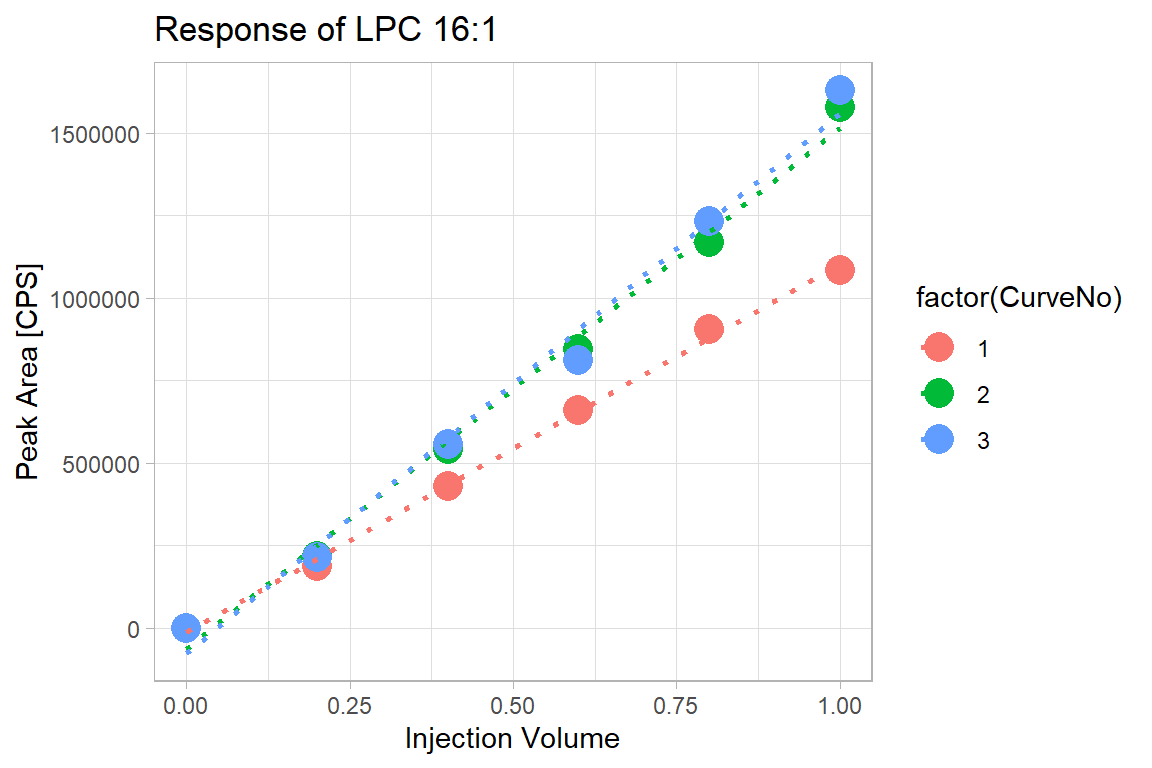
\includegraphics[width=18.75in,height=\textheight]{./plotting_basics_files/figure-pdf/plot-3-1.pdf}

}

\end{figure}

\hypertarget{faceted-plot-from-different-lipids-of-one-curve}{%
\section{Faceted plot from different lipids of one
curve}\label{faceted-plot-from-different-lipids-of-one-curve}}

\begin{Shaded}
\begin{Highlighting}[]
\CommentTok{\#Select data from all LPCs from  dilution curve 1}
\NormalTok{d\_forplot\_3 }\OtherTok{\textless{}{-}}\NormalTok{ d\_rqc  }\SpecialCharTok{|\textgreater{}} \FunctionTok{filter}\NormalTok{(}\FunctionTok{str\_detect}\NormalTok{(Lipid, }\StringTok{"LPC 2"}\NormalTok{), CurveNo }\SpecialCharTok{==} \DecValTok{2}\NormalTok{)}

\FunctionTok{ggplot}\NormalTok{(d\_forplot\_3, }\FunctionTok{aes}\NormalTok{(}\AttributeTok{x =}\NormalTok{ InjVol, }\AttributeTok{y =}\NormalTok{ Area, }\AttributeTok{color =} \FunctionTok{factor}\NormalTok{(CurveNo))) }\SpecialCharTok{+} 
  \FunctionTok{geom\_point}\NormalTok{(}\AttributeTok{size =} \DecValTok{2}\NormalTok{) }\SpecialCharTok{+}
  \FunctionTok{scale\_x\_continuous}\NormalTok{(}\AttributeTok{name =} \StringTok{"Injection Volume"}\NormalTok{, }\AttributeTok{limits =} \FunctionTok{c}\NormalTok{(}\DecValTok{0}\NormalTok{, }\ConstantTok{NA}\NormalTok{)) }\SpecialCharTok{+} 
  \FunctionTok{labs}\NormalTok{(}\AttributeTok{title =} \StringTok{"Response Curves"}\NormalTok{, }\AttributeTok{y =} \StringTok{"Peak Area [CPS]"}\NormalTok{) }\SpecialCharTok{+}
  \FunctionTok{geom\_smooth}\NormalTok{(}\AttributeTok{method =} \StringTok{"lm"}\NormalTok{, }\AttributeTok{se =} \ConstantTok{FALSE}\NormalTok{, }\AttributeTok{linetype =} \StringTok{"dotted"}\NormalTok{, }\AttributeTok{size =} \FloatTok{0.6}\NormalTok{) }\SpecialCharTok{+}
  \FunctionTok{facet\_wrap}\NormalTok{(}\SpecialCharTok{\textasciitilde{}}\NormalTok{Lipid, }\AttributeTok{scales =} \StringTok{"free"}\NormalTok{) }\SpecialCharTok{+}
  \FunctionTok{theme\_light}\NormalTok{(}\AttributeTok{base\_size =} \DecValTok{8}\NormalTok{)}
\end{Highlighting}
\end{Shaded}

\begin{figure}[H]

{\centering 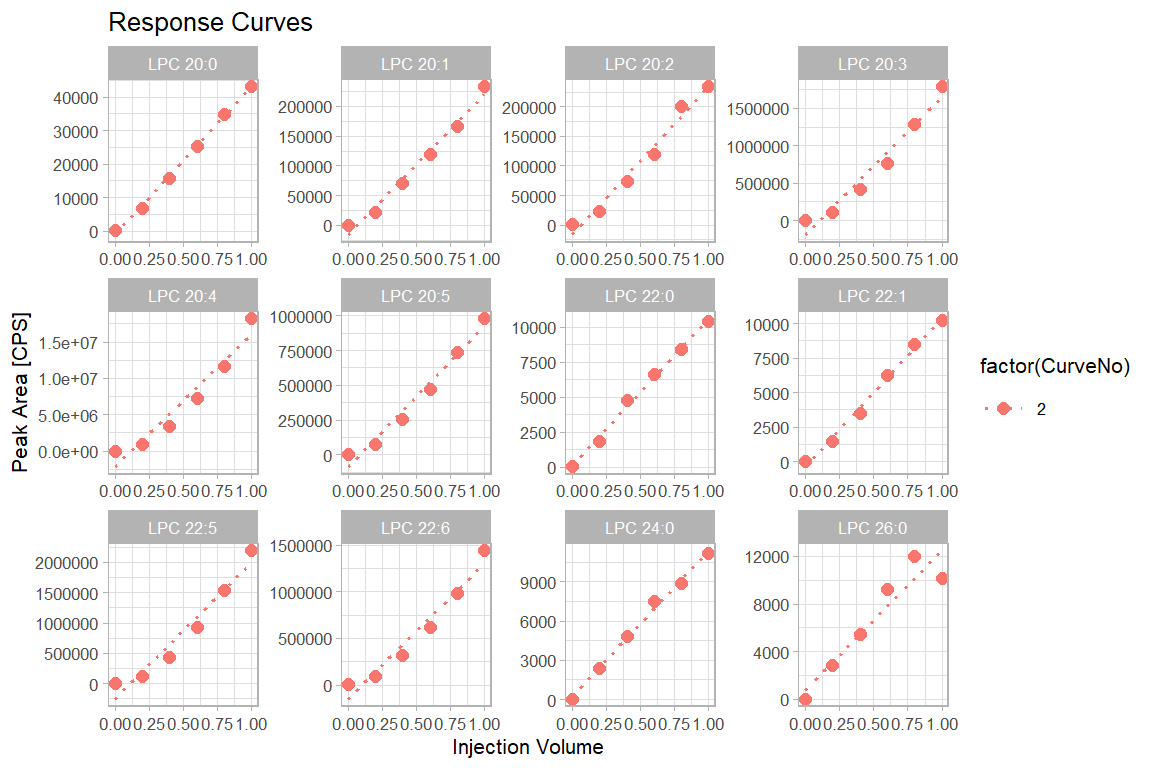
\includegraphics[width=18.75in,height=\textheight]{./plotting_basics_files/figure-pdf/plot-4-1.pdf}

}

\end{figure}

\hypertarget{add-r2-to-the-plots}{%
\section{\texorpdfstring{Add \(R^2\) to the
plots}{Add R\^{}2 to the plots}}\label{add-r2-to-the-plots}}

\begin{Shaded}
\begin{Highlighting}[]
\CommentTok{\# Plot}
\FunctionTok{ggplot}\NormalTok{(}\AttributeTok{data =}\NormalTok{ d\_forplot\_3, }\FunctionTok{aes}\NormalTok{(}\AttributeTok{x =}\NormalTok{ InjVol, }\AttributeTok{y =}\NormalTok{ Area, }
                               \AttributeTok{group =} \FunctionTok{factor}\NormalTok{(CurveNo))) }\SpecialCharTok{+}
  \FunctionTok{stat\_poly\_line}\NormalTok{() }\SpecialCharTok{+}
  \FunctionTok{stat\_poly\_eq}\NormalTok{(}
    \FunctionTok{aes}\NormalTok{(}
      \AttributeTok{label =} \FunctionTok{after\_stat}\NormalTok{(rr.label),}
      \AttributeTok{color =} \FunctionTok{if\_else}\NormalTok{(}\FunctionTok{after\_stat}\NormalTok{(r.squared) }\SpecialCharTok{\textless{}} \FloatTok{0.96}\NormalTok{, }\StringTok{"red"}\NormalTok{, }\StringTok{"black"}\NormalTok{)}
\NormalTok{    ),}
  \AttributeTok{size =} \FloatTok{2.4}\NormalTok{,}
  \AttributeTok{lineheight =} \FloatTok{1111.5}\NormalTok{) }\SpecialCharTok{+}
  \FunctionTok{scale\_color\_identity}\NormalTok{() }\SpecialCharTok{+}
  \FunctionTok{scale\_y\_continuous}\NormalTok{(}\AttributeTok{limits =} \FunctionTok{c}\NormalTok{(}\DecValTok{0}\NormalTok{, }\ConstantTok{NA}\NormalTok{)) }\SpecialCharTok{+}
  \FunctionTok{facet\_wrap}\NormalTok{( }\SpecialCharTok{\textasciitilde{}}\NormalTok{ Lipid, }\AttributeTok{scales =} \StringTok{"free"}\NormalTok{) }\SpecialCharTok{+}
  \FunctionTok{geom\_point}\NormalTok{() }\SpecialCharTok{+} \FunctionTok{theme\_light}\NormalTok{(}\AttributeTok{base\_size =} \DecValTok{6}\NormalTok{)}
\end{Highlighting}
\end{Shaded}

\begin{verbatim}
#> Warning: Removed 62 rows containing missing values (geom_smooth).
\end{verbatim}

\begin{figure}[H]

{\centering 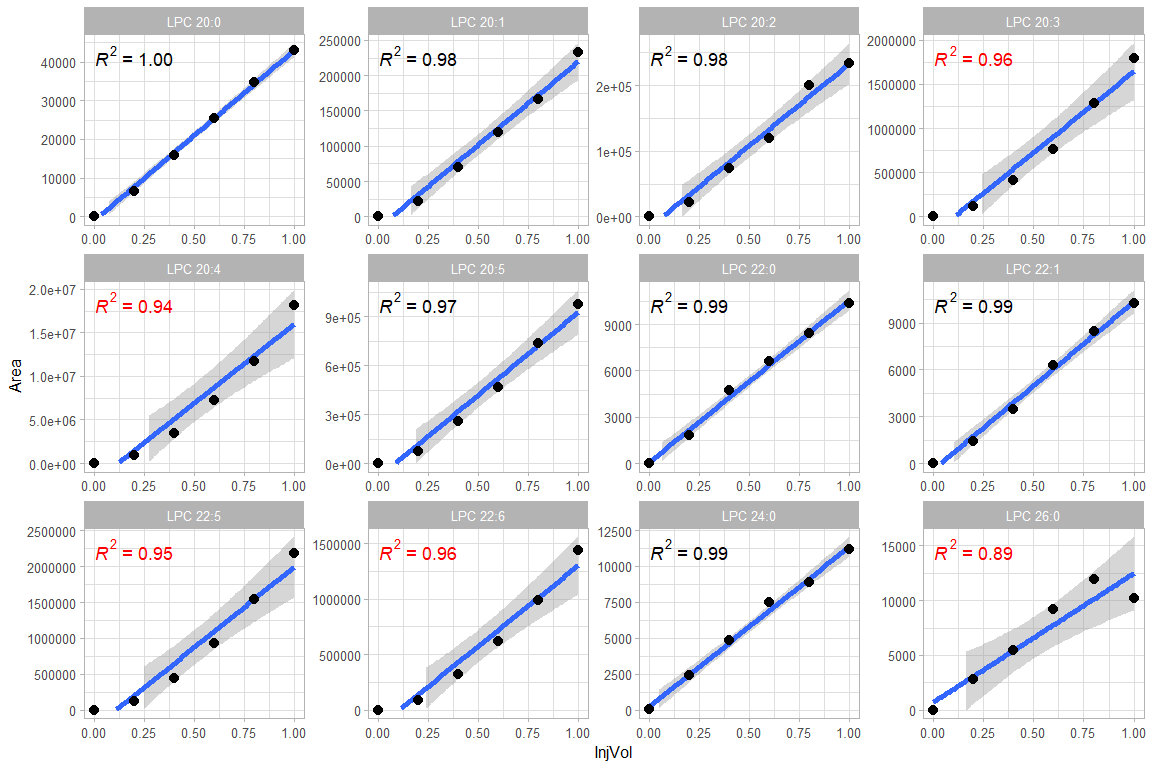
\includegraphics[width=18.75in,height=\textheight]{./plotting_basics_files/figure-pdf/plot-5-1.pdf}

}

\end{figure}

\hypertarget{faceted-plot-from-different-lipids-of-all-curves}{%
\section{Faceted plot from different lipids of all
curves}\label{faceted-plot-from-different-lipids-of-all-curves}}

\begin{Shaded}
\begin{Highlighting}[]
\CommentTok{\#Select data from all LPCs from  dilution curve 1}
\NormalTok{d\_forplot\_4 }\OtherTok{\textless{}{-}}\NormalTok{ d\_rqc  }\SpecialCharTok{|\textgreater{}} \FunctionTok{filter}\NormalTok{(}\FunctionTok{str\_detect}\NormalTok{(Lipid, }\StringTok{"LPC 2"}\NormalTok{))}

\FunctionTok{ggplot}\NormalTok{(d\_forplot\_4, }\FunctionTok{aes}\NormalTok{(}\AttributeTok{x =}\NormalTok{ InjVol, }\AttributeTok{y =}\NormalTok{ Area, }
                        \AttributeTok{color =} \FunctionTok{factor}\NormalTok{(CurveNo))) }\SpecialCharTok{+} 
  \FunctionTok{geom\_point}\NormalTok{(}\AttributeTok{size =} \DecValTok{2}\NormalTok{) }\SpecialCharTok{+}
  \FunctionTok{scale\_x\_continuous}\NormalTok{(}\AttributeTok{name =} \StringTok{"Injection Volume"}\NormalTok{, }\AttributeTok{limits =} \FunctionTok{c}\NormalTok{(}\DecValTok{0}\NormalTok{, }\ConstantTok{NA}\NormalTok{)) }\SpecialCharTok{+} 
  \FunctionTok{labs}\NormalTok{(}\AttributeTok{title =} \StringTok{"Response Curves"}\NormalTok{, }\AttributeTok{y =} \StringTok{"Peak Area [CPS]"}\NormalTok{) }\SpecialCharTok{+}
  \FunctionTok{geom\_smooth}\NormalTok{(}\AttributeTok{method =} \StringTok{"lm"}\NormalTok{, }\AttributeTok{se =} \ConstantTok{FALSE}\NormalTok{, }
              \AttributeTok{linetype =} \StringTok{"dotted"}\NormalTok{, }\AttributeTok{size =} \FloatTok{0.6}\NormalTok{) }\SpecialCharTok{+}
  \FunctionTok{facet\_wrap}\NormalTok{(}\SpecialCharTok{\textasciitilde{}}\NormalTok{Lipid, }\AttributeTok{scales =} \StringTok{"free"}\NormalTok{) }\SpecialCharTok{+}
  \FunctionTok{theme\_light}\NormalTok{(}\AttributeTok{base\_size =} \DecValTok{8}\NormalTok{)}
\end{Highlighting}
\end{Shaded}

\begin{figure}[H]

{\centering 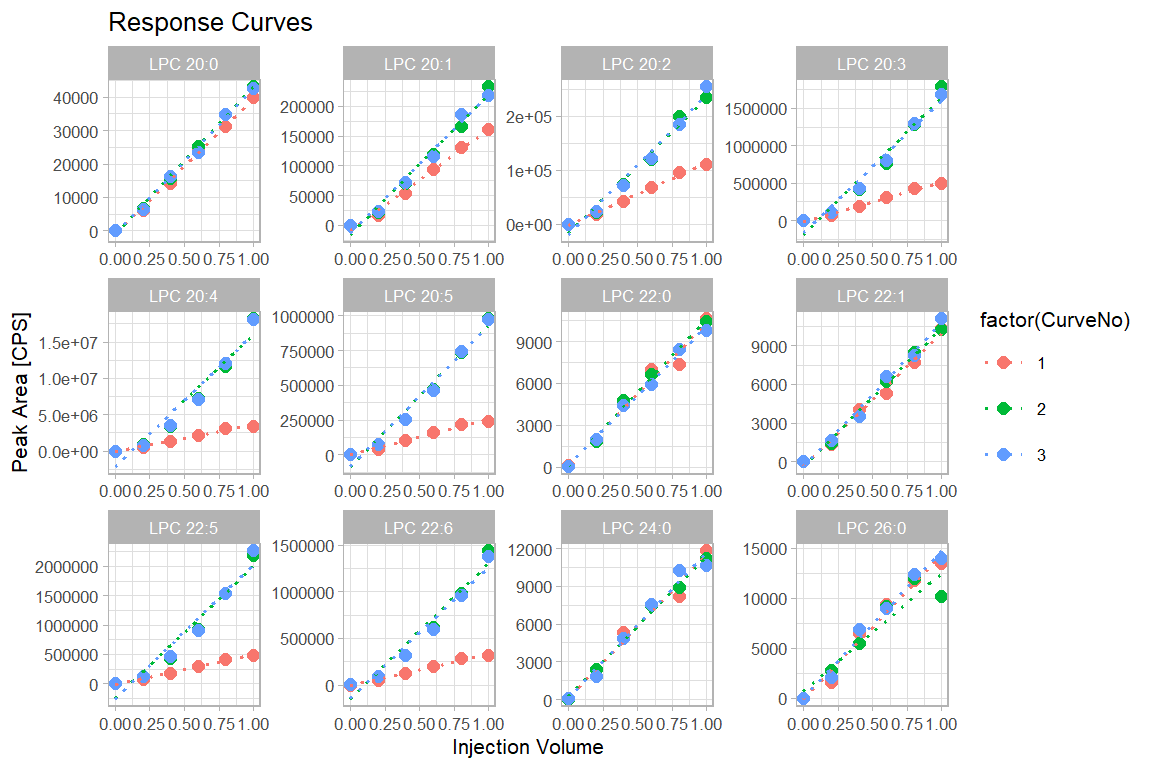
\includegraphics[width=18.75in,height=\textheight]{./plotting_basics_files/figure-pdf/plot-6-1.pdf}

}

\end{figure}

\hypertarget{faceted-plots-over-multiple-pages}{%
\section{Faceted plots over multiple
pages}\label{faceted-plots-over-multiple-pages}}

One option is to use `ggforce::facet\_wrap\_paginate()` but this
function can be slow and has some bugs with large datasets. Here an
alternative way using *purrr::map()*

\begin{Shaded}
\begin{Highlighting}[]
\CommentTok{\# Define function to plot 1 page}
\NormalTok{plot\_page }\OtherTok{\textless{}{-}}
  \ControlFlowTok{function}\NormalTok{(d, rows\_page, columns\_page) \{}
    \FunctionTok{ggplot}\NormalTok{(}\AttributeTok{data =}\NormalTok{ d, }\FunctionTok{aes}\NormalTok{(}\AttributeTok{x =}\NormalTok{ InjVol , }\AttributeTok{y =}\NormalTok{ Area, }\AttributeTok{group =} \FunctionTok{factor}\NormalTok{(CurveNo))) }\SpecialCharTok{+}
      \FunctionTok{stat\_poly\_line}\NormalTok{() }\SpecialCharTok{+}
      \FunctionTok{stat\_poly\_eq}\NormalTok{(}\FunctionTok{aes}\NormalTok{(}
        \AttributeTok{label =} \FunctionTok{after\_stat}\NormalTok{(rr.label),}
        \AttributeTok{color =} \FunctionTok{ifelse}\NormalTok{(}\FunctionTok{after\_stat}\NormalTok{(r.squared) }\SpecialCharTok{\textless{}} \FloatTok{0.80}\NormalTok{, }\StringTok{"red"}\NormalTok{, }\StringTok{"darkgreen"}\NormalTok{)}
\NormalTok{      ), }\AttributeTok{size =} \FloatTok{1.4}\NormalTok{) }\SpecialCharTok{+}
      \FunctionTok{scale\_color\_identity}\NormalTok{() }\SpecialCharTok{+}
      \FunctionTok{scale\_y\_continuous}\NormalTok{(}\AttributeTok{limits =} \FunctionTok{c}\NormalTok{(}\DecValTok{0}\NormalTok{, }\ConstantTok{NA}\NormalTok{)) }\SpecialCharTok{+}
      \FunctionTok{facet\_wrap}\NormalTok{(}\FunctionTok{vars}\NormalTok{(Lipid),}
      \AttributeTok{scales =} \StringTok{"free"}\NormalTok{,}
      \AttributeTok{nrow =}\NormalTok{ rows\_page,}
      \AttributeTok{ncol =}\NormalTok{ columns\_page) }\SpecialCharTok{+}
      \FunctionTok{geom\_point}\NormalTok{() }\SpecialCharTok{+} \FunctionTok{theme\_light}\NormalTok{(}\AttributeTok{base\_size =} \DecValTok{6}\NormalTok{)}
\NormalTok{  \}}

\CommentTok{\# Select all LPCs}
\NormalTok{d\_forplot\_5 }\OtherTok{\textless{}{-}}\NormalTok{ d\_rqc  }\SpecialCharTok{|\textgreater{}} \FunctionTok{filter}\NormalTok{(}\FunctionTok{str\_detect}\NormalTok{(Lipid, }\StringTok{"LPC "}\NormalTok{), CurveNo }\SpecialCharTok{==} \DecValTok{2}\NormalTok{)}

\CommentTok{\# Interate through pages}


\NormalTok{rows\_page }\OtherTok{=} \DecValTok{4}
\NormalTok{columns\_page }\OtherTok{=} \DecValTok{5}

\NormalTok{d\_rqc\_grp }\OtherTok{\textless{}{-}}\NormalTok{ d\_forplot\_5 }\SpecialCharTok{\%\textgreater{}\%}
  \FunctionTok{left\_join}\NormalTok{(}\FunctionTok{tibble}\NormalTok{(}\AttributeTok{Lipid =} \FunctionTok{unique}\NormalTok{(.}\SpecialCharTok{$}\NormalTok{Lipid)) }\SpecialCharTok{|\textgreater{}}
              \FunctionTok{mutate}\NormalTok{(}\AttributeTok{grp =} \FunctionTok{ceiling}\NormalTok{(}\FunctionTok{row\_number}\NormalTok{() }\SpecialCharTok{/}\NormalTok{ (rows\_page }\SpecialCharTok{*}\NormalTok{ columns\_page)))) }\SpecialCharTok{\%\textgreater{}\%}
  \FunctionTok{group\_by}\NormalTok{(grp) }\SpecialCharTok{\%\textgreater{}\%}
  \FunctionTok{nest}\NormalTok{() }\SpecialCharTok{\%\textgreater{}\%}
  \FunctionTok{mutate}\NormalTok{(}\AttributeTok{plt =} \FunctionTok{map}\NormalTok{(data, }\SpecialCharTok{\textasciitilde{}} \FunctionTok{plot\_page}\NormalTok{(.,}\AttributeTok{rows\_page =}\NormalTok{  rows\_page, }\AttributeTok{columns\_page =}  \DecValTok{5}\NormalTok{)))}

\CommentTok{\# Print pages }

\NormalTok{d\_rqc\_grp}\SpecialCharTok{$}\NormalTok{plt}
\end{Highlighting}
\end{Shaded}

\begin{verbatim}
#> Warning: Removed 101 rows containing missing values (geom_smooth).
\end{verbatim}

\begin{verbatim}
#> Warning: Removed 1 rows containing non-finite values (stat_poly_line).
\end{verbatim}

\begin{verbatim}
#> Warning: Removed 1 rows containing non-finite values (stat_poly_eq).
\end{verbatim}

\begin{verbatim}
#> Warning: Removed 56 rows containing missing values (geom_smooth).
\end{verbatim}

\begin{verbatim}
#> Warning: Removed 1 rows containing missing values (geom_point).
\end{verbatim}

\begin{figure}[H]

{\centering 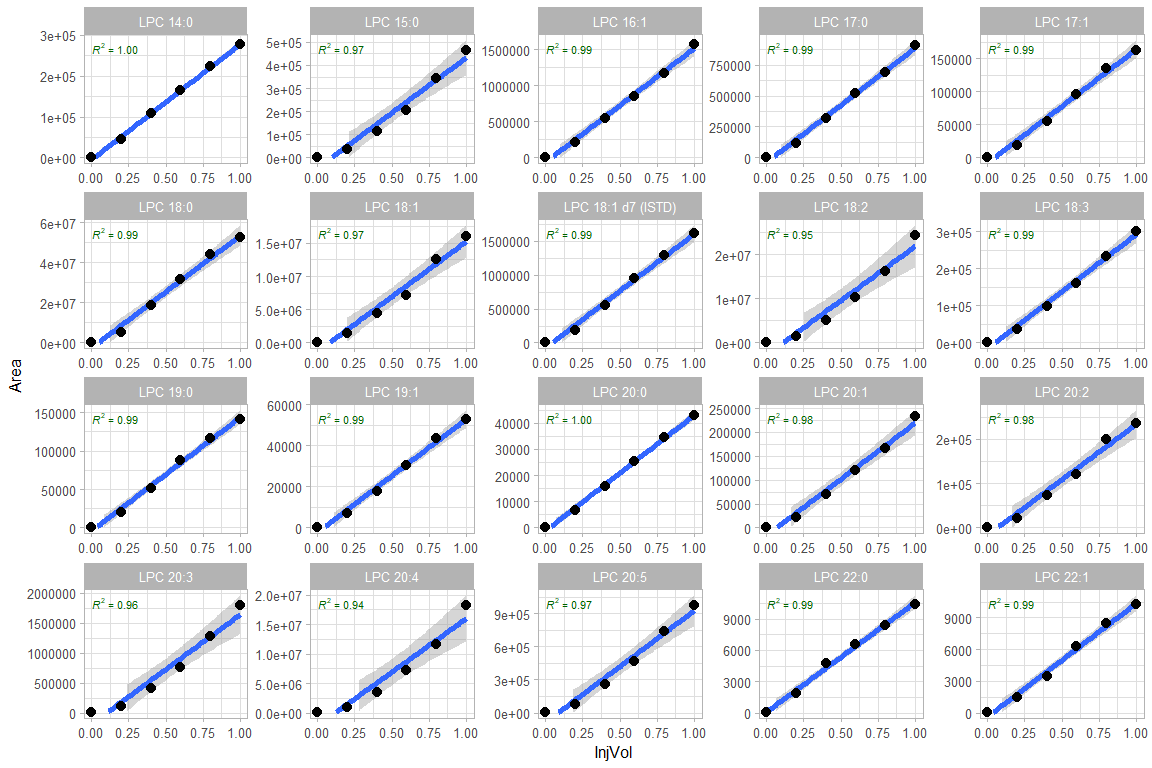
\includegraphics[width=18.75in,height=\textheight]{./plotting_basics_files/figure-pdf/plot-7-1.pdf}

}

\end{figure}

\begin{figure}[H]

{\centering 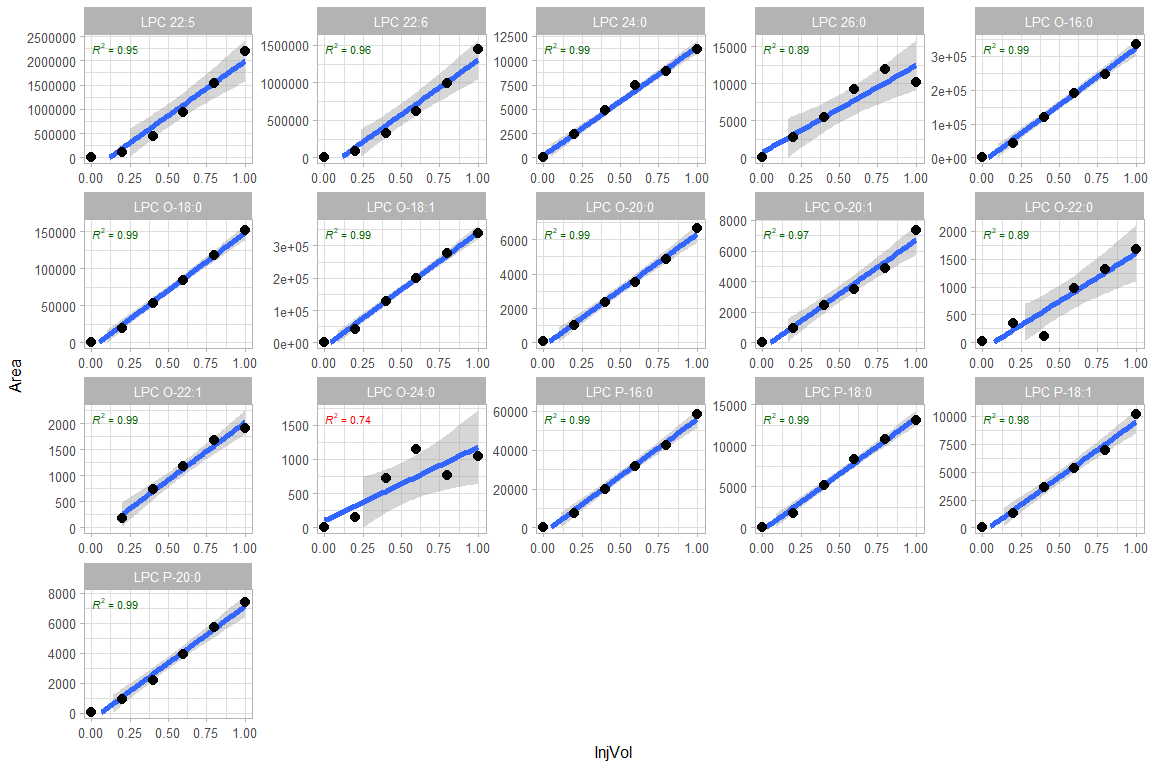
\includegraphics[width=18.75in,height=\textheight]{./plotting_basics_files/figure-pdf/plot-7-2.pdf}

}

\end{figure}

\hypertarget{save-multi-page-plot-a-pdf}{%
\section{Save multi-page plot a PDF}\label{save-multi-page-plot-a-pdf}}

\begin{Shaded}
\begin{Highlighting}[]
\FunctionTok{pdf}\NormalTok{(}\AttributeTok{file =} \StringTok{"dilutions.pdf"}\NormalTok{, }\AttributeTok{onefile =} \ConstantTok{TRUE}\NormalTok{, }\AttributeTok{paper =} \StringTok{"A4r"}\NormalTok{, }\AttributeTok{width =} \DecValTok{11}\NormalTok{)}
\NormalTok{d\_rqc\_grp}\SpecialCharTok{$}\NormalTok{plt}\SpecialCharTok{$}\NormalTok{plt}
\FunctionTok{dev.off}\NormalTok{()}
\end{Highlighting}
\end{Shaded}

\hypertarget{post-processingqc}{%
\chapter{Post-processing/QC}\label{post-processingqc}}

\hypertarget{libraries-1}{%
\section{Libraries}\label{libraries-1}}

\begin{Shaded}
\begin{Highlighting}[]
\FunctionTok{library}\NormalTok{(here)}
\FunctionTok{library}\NormalTok{(tidyverse)}
\end{Highlighting}
\end{Shaded}

\hypertarget{data-format}{%
\section{Data Format}\label{data-format}}

The examples below require a tidy (`long-format') table with following
columns: \texttt{DataFileName}, \texttt{Feature} and \texttt{Area}. See
chapters xxxx on how to prepare data in this format. For this chapter we
use the example data

\begin{Shaded}
\begin{Highlighting}[]
\CommentTok{\# Load and format test data}
\NormalTok{mydataset\_orig }\OtherTok{\textless{}{-}} \FunctionTok{read\_csv}\NormalTok{(}\FunctionTok{here}\NormalTok{(}\StringTok{"data/Testdata\_Lipidomics\_flat\_wide\_V3.csv"}\NormalTok{))}

\CommentTok{\# Convert to long format}
\NormalTok{mydataset }\OtherTok{\textless{}{-}}\NormalTok{ mydataset\_orig }\SpecialCharTok{|\textgreater{}} 
  \FunctionTok{pivot\_longer}\NormalTok{(}\SpecialCharTok{{-}}\NormalTok{DataFileName, }\AttributeTok{names\_to =} \StringTok{"Feature"}\NormalTok{, }\AttributeTok{values\_to =} \StringTok{"Area"}\NormalTok{)}
\end{Highlighting}
\end{Shaded}

Alternatively, to import a MassHunter CSV file you can use
\texttt{read\_MassHunterCSV} from the \texttt{SLINGtools}
(\url{https://slinghub.github.io/SLINGtools}) package

\begin{Shaded}
\begin{Highlighting}[]
\NormalTok{mydataset }\OtherTok{\textless{}{-}}\NormalTok{ SLINGtools}\SpecialCharTok{::}\FunctionTok{read\_MassHunterCSV}\NormalTok{(}
  \AttributeTok{file =} \FunctionTok{here}\NormalTok{(}\StringTok{"data/Testdata\_MHQuant\_Detailed\_V3.csv"}\NormalTok{))}
\end{Highlighting}
\end{Shaded}

\hypertarget{annotate}{%
\section{Annotate}\label{annotate}}

\begin{Shaded}
\begin{Highlighting}[]
\NormalTok{d }\OtherTok{\textless{}{-}}\NormalTok{ mydataset }\SpecialCharTok{|\textgreater{}} 
  \FunctionTok{select}\NormalTok{(DataFileName, }\AttributeTok{Lipid =}\NormalTok{ Feature, Area) }\SpecialCharTok{|\textgreater{}} 
  \FunctionTok{separate}\NormalTok{(}\AttributeTok{col =}\NormalTok{ DataFileName, }
           \AttributeTok{into =} \FunctionTok{c}\NormalTok{(}\StringTok{"ID"}\NormalTok{, }\StringTok{"QCtype"}\NormalTok{, }\StringTok{"SampleID"}\NormalTok{), }
           \AttributeTok{sep =} \StringTok{"\_"}\NormalTok{, }
           \AttributeTok{remove =} \ConstantTok{FALSE}\NormalTok{)}
\end{Highlighting}
\end{Shaded}

\hypertarget{runscatter}{%
\section{RunScatter}\label{runscatter}}

This is for one page (means one plot with n rows and m columns)

\part{Recipies}

\hypertarget{section}{%
\section*{}\label{section}}
\addcontentsline{toc}{section}{}

\hypertarget{bar-chart-with-contrasts}{%
\chapter{Bar chart with contrasts}\label{bar-chart-with-contrasts}}

Bar charts showing total composition per lipid class and statistical
comparisons between groups are still often seen in the literature.

\hypertarget{libraries-2}{%
\section{Libraries}\label{libraries-2}}

\begin{Shaded}
\begin{Highlighting}[]
\FunctionTok{library}\NormalTok{(here)}
\FunctionTok{library}\NormalTok{(tidyverse)}
\end{Highlighting}
\end{Shaded}

\hypertarget{data-format-1}{%
\section{Data format}\label{data-format-1}}

The example below requires a tidy (`long-format') table. Following
columns are will be used: \texttt{SubjectID}, \texttt{Group},
\texttt{LipidClass} and \texttt{Conc}. See chapters xxx on how to
prepare data in this format. For this example a raw test dataset will be
imported and converted into the tidy format. The the sum composition per
lipid classes is calculated and then provided to
\texttt{ggsignif::geom\_signif}.

\begin{Shaded}
\begin{Highlighting}[]
\NormalTok{d\_long }\OtherTok{\textless{}{-}} \FunctionTok{read\_csv}\NormalTok{(}\FunctionTok{here}\NormalTok{(}\StringTok{"data/Metabolites{-}1614644{-}supplementary.csv"}\NormalTok{)) }\SpecialCharTok{|\textgreater{}} 
  \FunctionTok{pivot\_longer}\NormalTok{(}\AttributeTok{cols =} \SpecialCharTok{{-}}\NormalTok{SubjectID}\SpecialCharTok{:{-}}\NormalTok{Group, }\AttributeTok{names\_to =} \StringTok{"Lipid"}\NormalTok{, }\AttributeTok{values\_to =} \StringTok{"Conc"}\NormalTok{)}

\NormalTok{d\_annot }\OtherTok{\textless{}{-}}\NormalTok{ d\_long }\SpecialCharTok{|\textgreater{}} 
  \FunctionTok{mutate}\NormalTok{(}\AttributeTok{Lipid =} \FunctionTok{str\_replace}\NormalTok{(Lipid, }\StringTok{" O{-}"}\NormalTok{, }\StringTok{"{-}O "}\NormalTok{), }
         \AttributeTok{Lipid =} \FunctionTok{str\_replace}\NormalTok{(Lipid, }\StringTok{" P{-}"}\NormalTok{, }\StringTok{"{-}P "}\NormalTok{)) }\SpecialCharTok{|\textgreater{}} 
  \FunctionTok{separate}\NormalTok{(}\AttributeTok{col =}\NormalTok{ Lipid, }\AttributeTok{into =} \FunctionTok{c}\NormalTok{(}\StringTok{"LipidClass"}\NormalTok{, }\StringTok{"chain"}\NormalTok{), }\AttributeTok{sep =} \StringTok{" "}\NormalTok{, }\AttributeTok{remove =} \ConstantTok{FALSE}\NormalTok{) }
\end{Highlighting}
\end{Shaded}

\begin{verbatim}
#> Warning: Expected 2 pieces. Additional pieces discarded in 376 rows [131, 132,
#> 183, 184, 419, 420, 471, 472, 707, 708, 759, 760, 995, 996, 1047, 1048, 1283,
#> 1284, 1335, 1336, ...].
\end{verbatim}

\begin{Shaded}
\begin{Highlighting}[]
\NormalTok{d\_sum }\OtherTok{\textless{}{-}}\NormalTok{ d\_annot }\SpecialCharTok{|\textgreater{}} 
  \FunctionTok{group\_by}\NormalTok{(SubjectID, Group, LipidClass) }\SpecialCharTok{|\textgreater{}} 
  \FunctionTok{summarise}\NormalTok{(}\AttributeTok{Conc =} \FunctionTok{sum}\NormalTok{(Conc)) }\SpecialCharTok{|\textgreater{}}  
  \FunctionTok{ungroup}\NormalTok{()}
\end{Highlighting}
\end{Shaded}

\hypertarget{tbl-data}{}
\begin{longtable}[]{@{}lllr@{}}
\caption{\label{tbl-data}Test dataset in tidy format}\tabularnewline
\toprule()
SubjectID & Group & LipidClass & Conc \\
\midrule()
\endfirsthead
\toprule()
SubjectID & Group & LipidClass & Conc \\
\midrule()
\endhead
CS\_01 & Cushing & CE & 12000.82 \\
CS\_01 & Cushing & Cer & 7.46 \\
CS\_01 & Cushing & DG & 76.85 \\
CS\_01 & Cushing & GM3 & 5.89 \\
CS\_01 & Cushing & Hex2Cer & 5.59 \\
\bottomrule()
\end{longtable}

\hypertarget{bar-chart-with-contrasts-1}{%
\section{Bar chart with contrasts}\label{bar-chart-with-contrasts-1}}

The display of significance brackets of statistical comparisons without
groups of a grouped bar chart needs a work- around when using the
\texttt{ggsignf} package. In this case the significance levels and
precise x and y coordinates have to be manually calculated and provided
to \texttt{ggsignif::geom\_signif}.

In this example below we use lipid class concentration normalized to the
reference group.

\begin{Shaded}
\begin{Highlighting}[]
\CommentTok{\# OPTIONAL: Subset you dataset}
\NormalTok{d\_plot }\OtherTok{\textless{}{-}}\NormalTok{ d\_sum  }\CommentTok{\# \%\textgreater{}\% filter(LipidClass \%in\% c("CE","TG","PC", "DG", "PE")) }


\CommentTok{\# OPTIONAL: Normalize your data (by e.g. the reference group)}
\NormalTok{d\_plot }\OtherTok{\textless{}{-}}\NormalTok{ d\_plot }\SpecialCharTok{|\textgreater{}}
  \FunctionTok{group\_by}\NormalTok{(LipidClass) }\SpecialCharTok{|\textgreater{}}
  \FunctionTok{mutate}\NormalTok{(}\AttributeTok{Conc =}\NormalTok{ Conc}\SpecialCharTok{/}\FunctionTok{mean}\NormalTok{(Conc[Group }\SpecialCharTok{==} \StringTok{"Healthy"}\NormalTok{]}\SpecialCharTok{/}\DecValTok{100}\NormalTok{))}
  
  
\CommentTok{\# OPTIONAL: order your groups as you wish (otherwise it will be alphabetical)}
\NormalTok{d\_plot}\SpecialCharTok{$}\NormalTok{Group }\OtherTok{\textless{}{-}} \FunctionTok{factor}\NormalTok{(d\_plot}\SpecialCharTok{$}\NormalTok{Group, }
                       \AttributeTok{levels =} \FunctionTok{c}\NormalTok{(}\StringTok{"Healthy"}\NormalTok{, }\StringTok{"Cushing"}\NormalTok{, }\StringTok{"Hypothyroidism"}\NormalTok{))}

\CommentTok{\# OPTIONAL: define specific color for each group, }
\NormalTok{my\_colors }\OtherTok{\textless{}{-}} \FunctionTok{c}\NormalTok{(}\AttributeTok{Healthy =} \StringTok{"grey80"}\NormalTok{, }\AttributeTok{Cushing =} \StringTok{"red"}\NormalTok{, }\AttributeTok{Hypothyroidism =} \StringTok{"\#1b80a1"}\NormalTok{)}


\CommentTok{\# }\AlertTok{NOTE}\CommentTok{: define your contrasts here, or select all combinations}
\CommentTok{\#contrasts \textless{}{-} list(c("Cushing", "Healthy"), c("Healthy","Hypothyroidism"))}
\NormalTok{contrasts }\OtherTok{\textless{}{-}} \FunctionTok{combn}\NormalTok{(}\FunctionTok{levels}\NormalTok{(d\_plot}\SpecialCharTok{$}\NormalTok{Group), }\DecValTok{2}\NormalTok{, }\AttributeTok{FUN =}\NormalTok{ list) }\CommentTok{\# All comb.}

\CommentTok{\# {-}{-}{-}{-} Get p{-}values and brackets coordinates  {-}{-}{-}{-}{-}}

\NormalTok{group\_levels }\OtherTok{\textless{}{-}} \FunctionTok{levels}\NormalTok{(d\_plot}\SpecialCharTok{$}\NormalTok{Group)}
\NormalTok{n\_groups }\OtherTok{\textless{}{-}} \FunctionTok{length}\NormalTok{(group\_levels)}

\NormalTok{get\_pval }\OtherTok{\textless{}{-}} \ControlFlowTok{function}\NormalTok{(d, contrasts) \{}
  \FunctionTok{map\_dfr}\NormalTok{(}\AttributeTok{.x =}\NormalTok{ contrasts,}
    \AttributeTok{.f =} \SpecialCharTok{\textasciitilde{}}\NormalTok{ broom}\SpecialCharTok{::}\FunctionTok{tidy}\NormalTok{(}
      \FunctionTok{t.test}\NormalTok{(}\AttributeTok{formula =}\NormalTok{ Conc }\SpecialCharTok{\textasciitilde{}} \FunctionTok{factor}\NormalTok{(Group),}\AttributeTok{data =} \FunctionTok{subset}\NormalTok{(d, Group }\SpecialCharTok{\%in\%}\NormalTok{ .x))) }\SpecialCharTok{|\textgreater{}}
      \FunctionTok{mutate}\NormalTok{(}\AttributeTok{id =} \FunctionTok{paste0}\NormalTok{(.x, }\AttributeTok{collapse =} \StringTok{"{-}"}\NormalTok{),}
             \AttributeTok{grp1 =}\NormalTok{ .x[}\DecValTok{1}\NormalTok{],}
             \AttributeTok{grp2 =}\NormalTok{ .x[}\DecValTok{2}\NormalTok{],}
             \AttributeTok{y\_max\_1 =} \FunctionTok{mean}\NormalTok{(d}\SpecialCharTok{$}\NormalTok{Conc[d}\SpecialCharTok{$}\NormalTok{Group }\SpecialCharTok{==}\NormalTok{ .x[}\DecValTok{1}\NormalTok{]])}\SpecialCharTok{+}\FunctionTok{sd}\NormalTok{(d}\SpecialCharTok{$}\NormalTok{Conc[d}\SpecialCharTok{$}\NormalTok{Group }\SpecialCharTok{==}\NormalTok{ .x[}\DecValTok{1}\NormalTok{]]),}
             \AttributeTok{y\_max\_2 =} \FunctionTok{mean}\NormalTok{(d}\SpecialCharTok{$}\NormalTok{Conc[d}\SpecialCharTok{$}\NormalTok{Group }\SpecialCharTok{==}\NormalTok{ .x[}\DecValTok{2}\NormalTok{]])}\SpecialCharTok{+}\FunctionTok{sd}\NormalTok{(d}\SpecialCharTok{$}\NormalTok{Conc[d}\SpecialCharTok{$}\NormalTok{Group }\SpecialCharTok{==}\NormalTok{ .x[}\DecValTok{2}\NormalTok{]]),}
             \AttributeTok{y\_max =} \FunctionTok{max}\NormalTok{(y\_max\_1, y\_max\_2)))}
\NormalTok{\}}

\NormalTok{d\_stat }\OtherTok{\textless{}{-}}\NormalTok{ d\_plot }\SpecialCharTok{|\textgreater{}}
  \FunctionTok{group\_by}\NormalTok{(LipidClass) }\SpecialCharTok{|\textgreater{}} 
  \FunctionTok{nest}\NormalTok{() }\SpecialCharTok{|\textgreater{}} 
  \FunctionTok{mutate}\NormalTok{(}\AttributeTok{res =} \FunctionTok{map}\NormalTok{(}\AttributeTok{.x =}\NormalTok{ data, }\AttributeTok{.f =}\NormalTok{ \textbackslash{}(x) }\AttributeTok{res =} \FunctionTok{get\_pval}\NormalTok{(x, contrasts))) }\SpecialCharTok{|\textgreater{}} 
  \FunctionTok{unnest}\NormalTok{(}\SpecialCharTok{{-}}\NormalTok{data) }\SpecialCharTok{|\textgreater{}} 
  \FunctionTok{mutate}\NormalTok{(}
    \AttributeTok{p\_val\_sym =} \FunctionTok{case\_when}\NormalTok{(}
\NormalTok{      p.value }\SpecialCharTok{\textgreater{}} \FloatTok{0.05} \SpecialCharTok{\textasciitilde{}} \StringTok{""}\NormalTok{, p.value }\SpecialCharTok{\textgreater{}} \FloatTok{0.01} \SpecialCharTok{\textasciitilde{}} \StringTok{"*"}\NormalTok{, }
\NormalTok{      p.value }\SpecialCharTok{\textgreater{}} \FloatTok{0.001} \SpecialCharTok{\textasciitilde{}} \StringTok{"**"}\NormalTok{, }\ConstantTok{TRUE} \SpecialCharTok{\textasciitilde{}} \StringTok{"***"}\NormalTok{))}\SpecialCharTok{|\textgreater{}}
  \FunctionTok{mutate}\NormalTok{(}\AttributeTok{y\_max =} \FunctionTok{max}\NormalTok{(y\_max)) }\SpecialCharTok{|\textgreater{}}
  \FunctionTok{ungroup}\NormalTok{() }\SpecialCharTok{|\textgreater{}} 
  \FunctionTok{mutate}\NormalTok{(}\AttributeTok{y\_max\_all =} \FunctionTok{max}\NormalTok{(y\_max)) }\SpecialCharTok{|\textgreater{}}
  \FunctionTok{group\_by}\NormalTok{(LipidClass) }\SpecialCharTok{|\textgreater{}} 
  \FunctionTok{mutate}\NormalTok{(}
    \AttributeTok{x\_min =} \FunctionTok{cur\_group\_id}\NormalTok{() }\SpecialCharTok{{-}} \FloatTok{0.8}\SpecialCharTok{/}\NormalTok{n\_groups }\SpecialCharTok{*}\NormalTok{ (}\FunctionTok{match}\NormalTok{(grp1, group\_levels)}\SpecialCharTok{{-}}\DecValTok{2}\NormalTok{),}
    \AttributeTok{x\_max =} \FunctionTok{cur\_group\_id}\NormalTok{() }\SpecialCharTok{{-}} \FloatTok{0.8}\SpecialCharTok{/}\NormalTok{n\_groups }\SpecialCharTok{*}\NormalTok{ (}\FunctionTok{match}\NormalTok{(grp2, group\_levels)}\SpecialCharTok{{-}}\DecValTok{2}\NormalTok{),}
    \AttributeTok{y\_max =}\NormalTok{ y\_max }\SpecialCharTok{+}\NormalTok{ (y\_max\_all}\SpecialCharTok{/}\DecValTok{30} \SpecialCharTok{*} \FunctionTok{row\_number}\NormalTok{() )}
\NormalTok{  )  }
\CommentTok{\# {-}{-}{-}{-} }\RegionMarkerTok{END}\CommentTok{ of Get p{-}values and brackets coordinates  {-}{-}{-}{-}{-}}

\CommentTok{\# The plotting function}
\NormalTok{plt }\OtherTok{\textless{}{-}} \FunctionTok{ggplot}\NormalTok{(d\_plot, }\FunctionTok{aes}\NormalTok{(}\AttributeTok{x =}\NormalTok{ LipidClass, }\AttributeTok{y =}\NormalTok{ Conc, }\AttributeTok{fill =}\NormalTok{ Group, }\AttributeTok{color =}\NormalTok{ Group)) }\SpecialCharTok{+} 
  \FunctionTok{geom\_hline}\NormalTok{(}\AttributeTok{yintercept =} \DecValTok{100}\NormalTok{, }\AttributeTok{color =} \StringTok{"green"}\NormalTok{, }\AttributeTok{size=}\FloatTok{0.1}\NormalTok{) }\SpecialCharTok{+}
  \FunctionTok{geom\_bar}\NormalTok{(}\AttributeTok{stat =} \StringTok{"summary"}\NormalTok{, }\AttributeTok{fun.data =} \StringTok{"mean\_sdl"}\NormalTok{, }
           \AttributeTok{position =} \StringTok{\textquotesingle{}dodge\textquotesingle{}}\NormalTok{, }\AttributeTok{width =} \FloatTok{0.8}\NormalTok{, }\AttributeTok{size  =} \DecValTok{0}\NormalTok{) }\SpecialCharTok{+}
  \FunctionTok{geom\_errorbar}\NormalTok{(}\AttributeTok{stat =} \StringTok{"summary"}\NormalTok{, }\AttributeTok{fun.data =} \StringTok{"mean\_sdl"}\NormalTok{, }\AttributeTok{fun.args =} \FunctionTok{list}\NormalTok{(}\AttributeTok{mult =} \DecValTok{1}\NormalTok{), }
                \AttributeTok{width =} \FloatTok{0.5}\NormalTok{, }\AttributeTok{position =} \FunctionTok{position\_dodge}\NormalTok{(}\AttributeTok{width=}\FloatTok{0.8}\NormalTok{), }\AttributeTok{size =} \FloatTok{0.1}\NormalTok{) }\SpecialCharTok{+} 
  \FunctionTok{scale\_y\_continuous}\NormalTok{(}\AttributeTok{limits =} \FunctionTok{c}\NormalTok{(}\DecValTok{0}\NormalTok{,}\ConstantTok{NA}\NormalTok{), }\AttributeTok{expand =} \FunctionTok{expansion}\NormalTok{(}\AttributeTok{mult =} \FunctionTok{c}\NormalTok{(}\DecValTok{0}\NormalTok{, .}\DecValTok{10}\NormalTok{)))}\SpecialCharTok{+}
  \FunctionTok{scale\_color\_manual}\NormalTok{(}\AttributeTok{values =}\NormalTok{ my\_colors) }\SpecialCharTok{+}
  \FunctionTok{scale\_fill\_manual}\NormalTok{(}\AttributeTok{values =}\NormalTok{ my\_colors) }\SpecialCharTok{+}

\NormalTok{  ggsignif}\SpecialCharTok{::}\FunctionTok{geom\_signif}\NormalTok{(}
    \AttributeTok{y\_position =}\NormalTok{ d\_stat}\SpecialCharTok{$}\NormalTok{y\_max,}
    \AttributeTok{xmin =}\NormalTok{ d\_stat}\SpecialCharTok{$}\NormalTok{x\_min,}
    \AttributeTok{xmax =}\NormalTok{ d\_stat}\SpecialCharTok{$}\NormalTok{x\_max,}
    \AttributeTok{annotation =}\NormalTok{ d\_stat}\SpecialCharTok{$}\NormalTok{p\_val\_sym,}
    \AttributeTok{margin\_top =} \FloatTok{0.05}\NormalTok{, }\AttributeTok{step\_increase =} \FloatTok{1.1}\NormalTok{, }\AttributeTok{vjust =} \FloatTok{0.5}\NormalTok{, }\AttributeTok{size =} \FloatTok{0.2}\NormalTok{,}
    \AttributeTok{tip\_length =} \FloatTok{0.005}\NormalTok{, }\AttributeTok{textsize =} \DecValTok{2}\NormalTok{, }\AttributeTok{color =} \StringTok{"black"}\NormalTok{) }\SpecialCharTok{+}
  \FunctionTok{theme\_light}\NormalTok{(}\AttributeTok{base\_size =} \DecValTok{8}\NormalTok{) }\SpecialCharTok{+} 
  \FunctionTok{theme}\NormalTok{(}
    \AttributeTok{axis.text.x =} \FunctionTok{element\_text}\NormalTok{( }\AttributeTok{size=}\DecValTok{9}\NormalTok{, }\AttributeTok{angle =} \DecValTok{45}\NormalTok{,}\AttributeTok{vjust =} \DecValTok{1}\NormalTok{, }\AttributeTok{hjust =} \DecValTok{1}\NormalTok{),}
    \AttributeTok{panel.grid =} \FunctionTok{element\_blank}\NormalTok{(),}
    \AttributeTok{legend.key.size =} \FunctionTok{unit}\NormalTok{(}\DecValTok{3}\NormalTok{,}\AttributeTok{units =} \StringTok{"mm"}\NormalTok{),}
    \CommentTok{\#legend.position=c(0.93, .87),}
    \AttributeTok{legend.title=}\FunctionTok{element\_blank}\NormalTok{()) }\SpecialCharTok{+}
  \FunctionTok{ylab}\NormalTok{(}\StringTok{"Relative abundance vs Reference"}\NormalTok{)}

\NormalTok{plt  }

\CommentTok{\#ggsave(plot = plt, filename = "barchart.png", }
\CommentTok{\#       width = 183, height = 90,units = "mm",  dpi = 300)}
\end{Highlighting}
\end{Shaded}

\begin{figure}[H]

{\centering 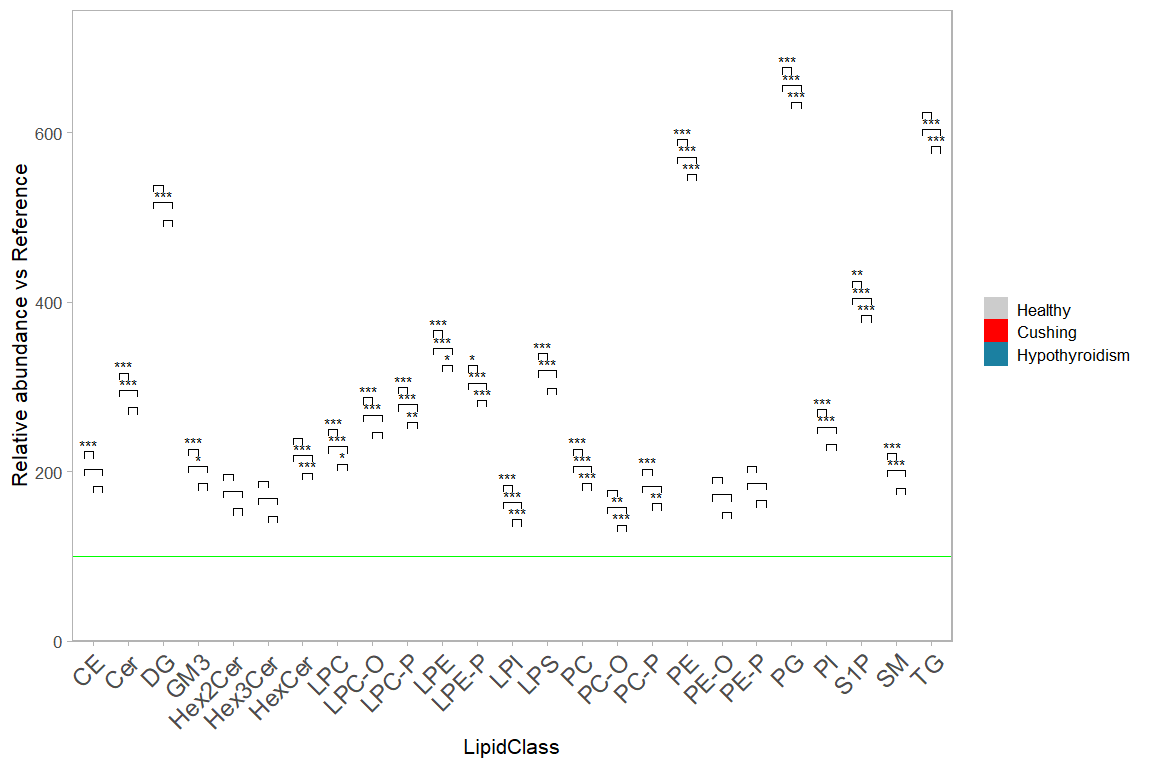
\includegraphics[width=18.75in,height=\textheight]{./barchart_lipidomics_files/figure-pdf/plot-barchart-1.pdf}

}

\end{figure}

Compare this to plotting non-normalized concentrations

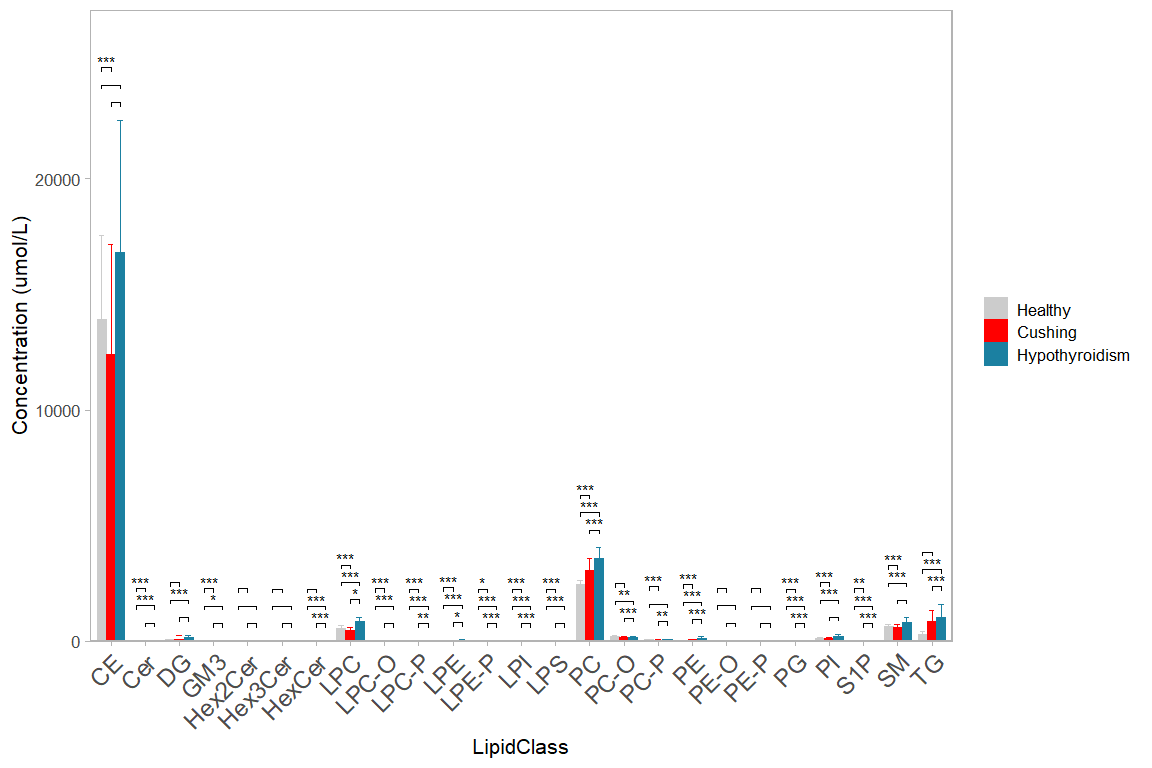
\includegraphics[width=18.75in,height=\textheight]{./barchart_lipidomics_files/figure-pdf/plot-barchart2-1.pdf}

\hypertarget{boxdot-plots-with-contrasts}{%
\chapter{Box/dot plots with
Contrasts}\label{boxdot-plots-with-contrasts}}

\hypertarget{libraries-3}{%
\section{Libraries}\label{libraries-3}}

\begin{Shaded}
\begin{Highlighting}[]
\FunctionTok{library}\NormalTok{(here)}
\FunctionTok{library}\NormalTok{(tidyverse)}
\end{Highlighting}
\end{Shaded}

\hypertarget{data-format-2}{%
\section{Data Format}\label{data-format-2}}

The examples below require a tidy (`long-format') table with following
columns: \texttt{SubjectID}, \texttt{Group}, \texttt{Lipid} and
\texttt{Conc}. See chapters xxxx on how to prepare data in this format.
In this example a test dataset is used that is converted into the tidy
format.

\begin{Shaded}
\begin{Highlighting}[]
\CommentTok{\# Load and format test data}
\NormalTok{d\_long }\OtherTok{\textless{}{-}} \FunctionTok{read\_csv}\NormalTok{(}\FunctionTok{here}\NormalTok{(}\StringTok{"data/Metabolites{-}1614644{-}supplementary.csv"}\NormalTok{)) }\SpecialCharTok{|\textgreater{}} 
  \FunctionTok{pivot\_longer}\NormalTok{(}\AttributeTok{cols =} \SpecialCharTok{{-}}\FunctionTok{c}\NormalTok{(SubjectID, Group), }\AttributeTok{names\_to =} \StringTok{"Lipid"}\NormalTok{, }\AttributeTok{values\_to =} \StringTok{"Conc"}\NormalTok{)}
\end{Highlighting}
\end{Shaded}

\hypertarget{tbl-data}{}
\begin{longtable}[]{@{}lllr@{}}
\caption{\label{tbl-data}Test data in tidy format}\tabularnewline
\toprule()
SubjectID & Group & Lipid & Conc \\
\midrule()
\endfirsthead
\toprule()
SubjectID & Group & Lipid & Conc \\
\midrule()
\endhead
HB\_01 & Healthy & CE 16:0 & 36.82 \\
HB\_01 & Healthy & CE 17:0 & 1.02 \\
HB\_01 & Healthy & CE 17:1 & 1.34 \\
HB\_01 & Healthy & CE 18:0 & 12.34 \\
HB\_01 & Healthy & CE 18:1 & 573.83 \\
\bottomrule()
\end{longtable}

\hypertarget{single-faceted-boxdot-plot}{%
\section{Single faceted box/dot plot}\label{single-faceted-boxdot-plot}}

This is for one page (means one plot with n rows and m columns)

\begin{Shaded}
\begin{Highlighting}[]
\CommentTok{\# OPTIONAL: order your groups as you wish (otherwise it will be alphabetical)}
\NormalTok{d\_long}\SpecialCharTok{$}\NormalTok{Group }\OtherTok{\textless{}{-}} \FunctionTok{factor}\NormalTok{(d\_long}\SpecialCharTok{$}\NormalTok{Group, }
                       \AttributeTok{levels =} \FunctionTok{c}\NormalTok{(}\StringTok{"Healthy"}\NormalTok{, }\StringTok{"Cushing"}\NormalTok{, }\StringTok{"Hypothyroidism"}\NormalTok{))}

\CommentTok{\# OPTIONAL: define specific color for each group, }
\NormalTok{my\_colors }\OtherTok{\textless{}{-}} \FunctionTok{c}\NormalTok{(}\AttributeTok{Healthy =} \StringTok{"grey50"}\NormalTok{, }\AttributeTok{Cushing =} \StringTok{"red"}\NormalTok{, }\AttributeTok{Hypothyroidism =} \StringTok{"\#1b80a1"}\NormalTok{)}

\CommentTok{\# OPTIONAL: Subset your data}
\NormalTok{d\_plot }\OtherTok{\textless{}{-}}\NormalTok{ d\_long }\SpecialCharTok{|\textgreater{}} \FunctionTok{filter}\NormalTok{(}\FunctionTok{str\_detect}\NormalTok{(Lipid, }\StringTok{"CE"}\NormalTok{))}


\CommentTok{\# IMPORTANT: Change variable names to match your data (i.e. Group, Conc, Lipid)}
\CommentTok{\# IMPORTANT: Change group names and add/remove comparisons in \textasciigrave{}ggsignif()\textasciigrave{}}
\FunctionTok{ggplot}\NormalTok{(d\_plot, }\FunctionTok{aes}\NormalTok{(}\AttributeTok{x =}\NormalTok{ Group, }\AttributeTok{y =}\NormalTok{ Conc, }\AttributeTok{color =}\NormalTok{ Group,}\AttributeTok{fill =}\NormalTok{ Group)) }\SpecialCharTok{+} 
  \FunctionTok{geom\_boxplot}\NormalTok{(}\AttributeTok{alpha =} \FloatTok{0.2}\NormalTok{, }\AttributeTok{lwd=}\FloatTok{0.3}\NormalTok{, }\AttributeTok{outlier.shape =} \ConstantTok{NA}\NormalTok{) }\SpecialCharTok{+}
  \FunctionTok{geom\_jitter}\NormalTok{(}\AttributeTok{size =} \FloatTok{0.5}\NormalTok{,}\AttributeTok{width =} \FloatTok{0.2}\NormalTok{) }\SpecialCharTok{+}
  \FunctionTok{facet\_wrap}\NormalTok{(}\SpecialCharTok{\textasciitilde{}}\NormalTok{Lipid, }\AttributeTok{scales =} \StringTok{"free"}\NormalTok{, }\AttributeTok{nrow =} \DecValTok{4}\NormalTok{, }\AttributeTok{ncol =} \DecValTok{5}\NormalTok{) }\SpecialCharTok{+} 
  \FunctionTok{scale\_y\_continuous}\NormalTok{(}\AttributeTok{limits =} \FunctionTok{c}\NormalTok{(}\DecValTok{0}\NormalTok{,}\ConstantTok{NA}\NormalTok{), }\AttributeTok{expand =} \FunctionTok{expansion}\NormalTok{(}\AttributeTok{mult =} \FunctionTok{c}\NormalTok{(}\DecValTok{0}\NormalTok{, .}\DecValTok{15}\NormalTok{)))}\SpecialCharTok{+}
  \FunctionTok{scale\_color\_manual}\NormalTok{(}\AttributeTok{values =}\NormalTok{ my\_colors) }\SpecialCharTok{+}
  \FunctionTok{scale\_fill\_manual}\NormalTok{(}\AttributeTok{values =}\NormalTok{ my\_colors) }\SpecialCharTok{+}
\NormalTok{  ggsignif}\SpecialCharTok{::}\FunctionTok{geom\_signif}\NormalTok{(}
    \AttributeTok{comparisons =} \FunctionTok{list}\NormalTok{(}
      \FunctionTok{c}\NormalTok{(}\StringTok{"Healthy"}\NormalTok{, }\StringTok{"Cushing"}\NormalTok{) ,}
      \FunctionTok{c}\NormalTok{(}\StringTok{"Cushing"}\NormalTok{, }\StringTok{"Hypothyroidism"}\NormalTok{), }
      \FunctionTok{c}\NormalTok{(}\StringTok{"Healthy"}\NormalTok{, }\StringTok{"Hypothyroidism"}\NormalTok{)}
\NormalTok{    ), }
    \AttributeTok{test =} \StringTok{"t.test"}\NormalTok{, }
    \AttributeTok{test.args =} \FunctionTok{list}\NormalTok{(}\AttributeTok{paired=}\ConstantTok{FALSE}\NormalTok{, }\AttributeTok{var.equal =} \ConstantTok{FALSE}\NormalTok{, }\AttributeTok{na.rm =} \ConstantTok{TRUE}\NormalTok{), }
    \AttributeTok{map\_signif\_level =} \FunctionTok{c}\NormalTok{(}\StringTok{"***"}\OtherTok{=}\FloatTok{0.001}\NormalTok{, }\StringTok{"**"}\OtherTok{=}\FloatTok{0.01}\NormalTok{, }\StringTok{"*"}\OtherTok{=}\FloatTok{0.05}\NormalTok{, }\StringTok{" "} \OtherTok{=} \DecValTok{1}\NormalTok{),}
    \AttributeTok{margin\_top =} \FloatTok{0.05}\NormalTok{, }\AttributeTok{step\_increase =} \FloatTok{0.1}\NormalTok{, }\AttributeTok{vjust =} \FloatTok{0.5}\NormalTok{, }\AttributeTok{size =} \FloatTok{0.2}\NormalTok{, }
    \AttributeTok{tip\_length =} \FloatTok{0.05}\NormalTok{, }\AttributeTok{textsize =} \DecValTok{4}\NormalTok{, }\AttributeTok{color =} \StringTok{"black"}\NormalTok{) }\SpecialCharTok{+}
  \FunctionTok{theme\_bw}\NormalTok{(}\AttributeTok{base\_size =} \DecValTok{7}\NormalTok{) }\SpecialCharTok{+} 
  \FunctionTok{theme}\NormalTok{(}
    \AttributeTok{axis.text.x =} \FunctionTok{element\_text}\NormalTok{( }\AttributeTok{size=}\DecValTok{6}\NormalTok{, }\AttributeTok{angle =} \DecValTok{45}\NormalTok{,}\AttributeTok{vjust =} \DecValTok{1}\NormalTok{, }\AttributeTok{hjust =} \DecValTok{1}\NormalTok{),}
    \AttributeTok{panel.grid =} \FunctionTok{element\_blank}\NormalTok{(),}
    \AttributeTok{legend.position=}\StringTok{"none"}
\NormalTok{  )}
\end{Highlighting}
\end{Shaded}

\begin{figure}[H]

{\centering \includegraphics[width=18.75in,height=\textheight]{./dotplot_lipidomics_files/figure-pdf/plot-1-1.pdf}

}

\end{figure}

\hypertarget{multi-page-faceted-boxdot-plot}{%
\section{Multi-page faceted box/dot
plot}\label{multi-page-faceted-boxdot-plot}}

Here we make the same plots as before but over multiple pages/figures,
like this we can make boxplots for each lipid If you adopt this for your
own data, you need to set number of plots per page (number of rows and
columns), also you need to update it with your group names and colors.

\begin{Shaded}
\begin{Highlighting}[]
\CommentTok{\# Order the groups as you wish (otherwise it will be alphabetical), if you are }
\NormalTok{d\_long}\SpecialCharTok{$}\NormalTok{Group }\OtherTok{\textless{}{-}} \FunctionTok{factor}\NormalTok{(d\_long}\SpecialCharTok{$}\NormalTok{Group, }
                       \AttributeTok{levels =} \FunctionTok{c}\NormalTok{(}\StringTok{"Healthy"}\NormalTok{, }\StringTok{"Cushing"}\NormalTok{, }\StringTok{"Hypothyroidism"}\NormalTok{))}

\CommentTok{\# Define your color for each group, }
\CommentTok{\# can also get colors (e.g. \#1b80a1) via e.g. https://g.co/kgs/DQH6Fr}
\NormalTok{my\_colors }\OtherTok{\textless{}{-}} \FunctionTok{c}\NormalTok{(}\AttributeTok{Healthy =} \StringTok{"grey50"}\NormalTok{, }\AttributeTok{Cushing =} \StringTok{"red"}\NormalTok{, }\AttributeTok{Hypothyroidism =} \StringTok{"\#1b80a1"}\NormalTok{)}


\CommentTok{\# In this example we subet to have 3 pages, remove the filter for all lipids}
\NormalTok{d\_plot }\OtherTok{\textless{}{-}}\NormalTok{ d\_long }\SpecialCharTok{|\textgreater{}} \FunctionTok{filter}\NormalTok{(}\FunctionTok{str\_detect}\NormalTok{(Lipid, }\StringTok{"LPC|LPE"}\NormalTok{))}

\CommentTok{\# Define a function to plot one faceted plot (=one page)}
\NormalTok{plot\_one\_page }\OtherTok{\textless{}{-}} \ControlFlowTok{function}\NormalTok{(data, n\_row, n\_col)\{}
  \FunctionTok{ggplot}\NormalTok{(data, }\FunctionTok{aes}\NormalTok{(}\AttributeTok{x =}\NormalTok{ Group, }\AttributeTok{y =}\NormalTok{ Conc, }\AttributeTok{color =}\NormalTok{ Group,}\AttributeTok{fill =}\NormalTok{ Group)) }\SpecialCharTok{+} 
    \FunctionTok{geom\_boxplot}\NormalTok{(}\AttributeTok{alpha =} \FloatTok{0.2}\NormalTok{, }\AttributeTok{lwd=}\FloatTok{0.3}\NormalTok{, }\AttributeTok{outlier.shape =} \ConstantTok{NA}\NormalTok{) }\SpecialCharTok{+}
    \FunctionTok{geom\_jitter}\NormalTok{(}\AttributeTok{size =} \FloatTok{0.5}\NormalTok{,}\AttributeTok{width =} \FloatTok{0.2}\NormalTok{) }\SpecialCharTok{+}
    \FunctionTok{facet\_wrap}\NormalTok{(}\SpecialCharTok{\textasciitilde{}}\NormalTok{Lipid, }\AttributeTok{scales =} \StringTok{"free"}\NormalTok{, }\AttributeTok{nrow =}\NormalTok{ n\_row, }\AttributeTok{ncol =}\NormalTok{ n\_col) }\SpecialCharTok{+} 
    \FunctionTok{scale\_y\_continuous}\NormalTok{(}\AttributeTok{limits =} \FunctionTok{c}\NormalTok{(}\DecValTok{0}\NormalTok{,}\ConstantTok{NA}\NormalTok{), }\AttributeTok{expand =} \FunctionTok{expansion}\NormalTok{(}\AttributeTok{mult =} \FunctionTok{c}\NormalTok{(}\DecValTok{0}\NormalTok{, .}\DecValTok{15}\NormalTok{)))}\SpecialCharTok{+}
    \FunctionTok{scale\_color\_manual}\NormalTok{(}\AttributeTok{values =}\NormalTok{ my\_colors) }\SpecialCharTok{+}
    \FunctionTok{scale\_fill\_manual}\NormalTok{(}\AttributeTok{values =}\NormalTok{ my\_colors) }\SpecialCharTok{+}
\NormalTok{    ggsignif}\SpecialCharTok{::}\FunctionTok{geom\_signif}\NormalTok{(}
      \AttributeTok{comparisons =} \FunctionTok{list}\NormalTok{(}
        \FunctionTok{c}\NormalTok{(}\StringTok{"Healthy"}\NormalTok{, }\StringTok{"Cushing"}\NormalTok{) ,}
        \FunctionTok{c}\NormalTok{(}\StringTok{"Cushing"}\NormalTok{, }\StringTok{"Hypothyroidism"}\NormalTok{), }
        \FunctionTok{c}\NormalTok{(}\StringTok{"Healthy"}\NormalTok{, }\StringTok{"Hypothyroidism"}\NormalTok{)}
\NormalTok{      ), }
      \AttributeTok{test =} \StringTok{"t.test"}\NormalTok{, }
      \AttributeTok{test.args =} \FunctionTok{list}\NormalTok{(}\AttributeTok{paired=}\ConstantTok{FALSE}\NormalTok{, }\AttributeTok{var.equal =} \ConstantTok{FALSE}\NormalTok{, }\AttributeTok{na.rm =} \ConstantTok{TRUE}\NormalTok{), }
      \AttributeTok{map\_signif\_level =} \FunctionTok{c}\NormalTok{(}\StringTok{"***"}\OtherTok{=}\FloatTok{0.001}\NormalTok{, }\StringTok{"**"}\OtherTok{=}\FloatTok{0.01}\NormalTok{, }\StringTok{"*"}\OtherTok{=}\FloatTok{0.05}\NormalTok{, }\StringTok{" "} \OtherTok{=} \DecValTok{1}\NormalTok{),}
      \AttributeTok{margin\_top =} \FloatTok{0.05}\NormalTok{, }\AttributeTok{step\_increase =} \FloatTok{0.1}\NormalTok{, }\AttributeTok{vjust =} \FloatTok{0.5}\NormalTok{, }\AttributeTok{size =} \FloatTok{0.2}\NormalTok{, }
      \AttributeTok{tip\_length =} \FloatTok{0.05}\NormalTok{, }\AttributeTok{textsize =} \DecValTok{4}\NormalTok{, }\AttributeTok{color =} \StringTok{"black"}\NormalTok{) }\SpecialCharTok{+}
    \FunctionTok{theme\_bw}\NormalTok{(}\AttributeTok{base\_size =} \DecValTok{7}\NormalTok{) }\SpecialCharTok{+} 
    \FunctionTok{theme}\NormalTok{(}
      \AttributeTok{axis.text.x =} \FunctionTok{element\_text}\NormalTok{( }\AttributeTok{size=}\DecValTok{6}\NormalTok{, }\AttributeTok{angle =} \DecValTok{45}\NormalTok{,}\AttributeTok{vjust =} \DecValTok{1}\NormalTok{, }\AttributeTok{hjust =} \DecValTok{1}\NormalTok{),}
      \AttributeTok{panel.grid =} \FunctionTok{element\_blank}\NormalTok{(),}
      \AttributeTok{legend.position=}\StringTok{"none"}
\NormalTok{    )}
\NormalTok{\}}

\CommentTok{\# Set how many plots per page (number of rows and columns)}
\NormalTok{rows\_page }\OtherTok{=} \DecValTok{3}
\NormalTok{columns\_page }\OtherTok{=} \DecValTok{5}

\NormalTok{my\_plots }\OtherTok{\textless{}{-}}\NormalTok{ d\_plot }\SpecialCharTok{\%\textgreater{}\%}
  \FunctionTok{group\_by}\NormalTok{(Lipid) }\SpecialCharTok{|\textgreater{}} 
  \FunctionTok{mutate}\NormalTok{(}\AttributeTok{page\_no =} \FunctionTok{ceiling}\NormalTok{(}\FunctionTok{cur\_group\_id}\NormalTok{()}\SpecialCharTok{/}\NormalTok{ (rows\_page }\SpecialCharTok{*}\NormalTok{ columns\_page))) }\SpecialCharTok{|\textgreater{}} 
  \FunctionTok{group\_by}\NormalTok{(page\_no) }\SpecialCharTok{\%\textgreater{}\%}
  \FunctionTok{nest}\NormalTok{() }\SpecialCharTok{\%\textgreater{}\%}
  \FunctionTok{mutate}\NormalTok{(}\AttributeTok{plt =} \FunctionTok{map}\NormalTok{(data, }\SpecialCharTok{\textasciitilde{}} \FunctionTok{plot\_one\_page}\NormalTok{(.,}\AttributeTok{n\_row =}\NormalTok{ rows\_page, }\AttributeTok{n\_col =}\NormalTok{ columns\_page)))}

\NormalTok{my\_plots}\SpecialCharTok{$}\NormalTok{plt}
\end{Highlighting}
\end{Shaded}

\begin{figure}[H]

{\centering \includegraphics[width=18.75in,height=\textheight]{./dotplot_lipidomics_files/figure-pdf/plot-2-1.pdf}

}

\end{figure}

\begin{figure}[H]

{\centering 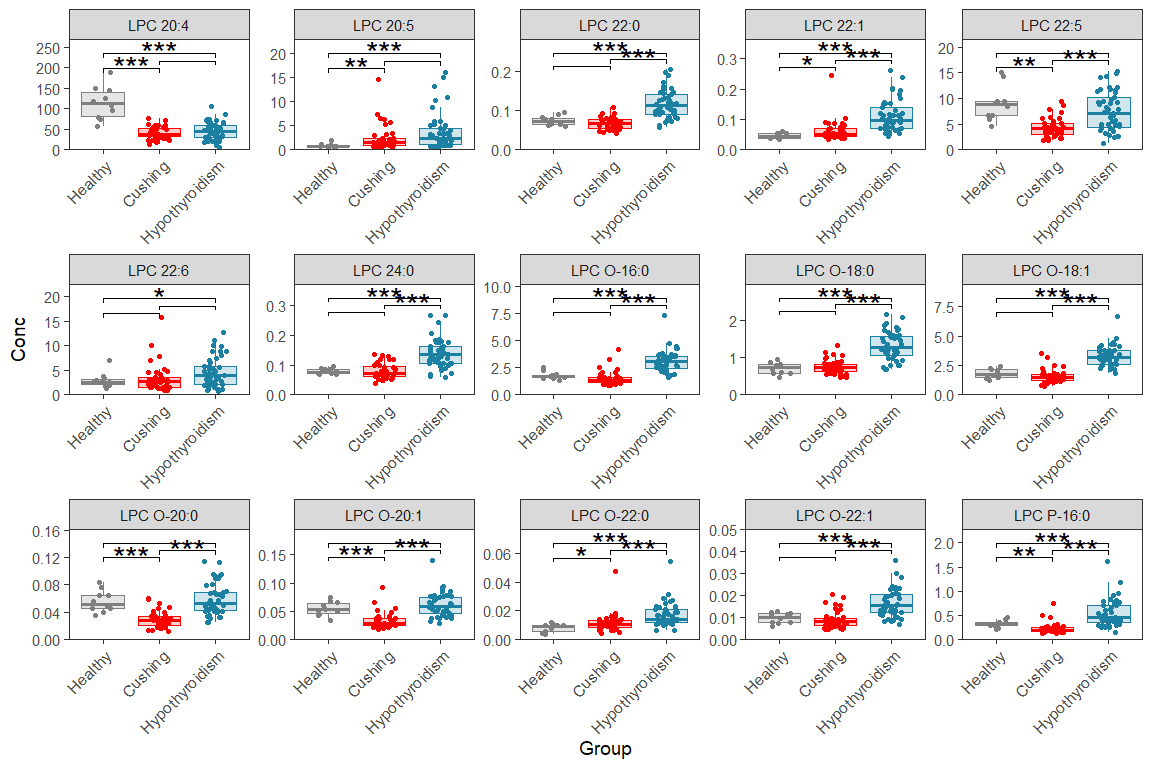
\includegraphics[width=18.75in,height=\textheight]{./dotplot_lipidomics_files/figure-pdf/plot-2-2.pdf}

}

\end{figure}

\begin{figure}[H]

{\centering 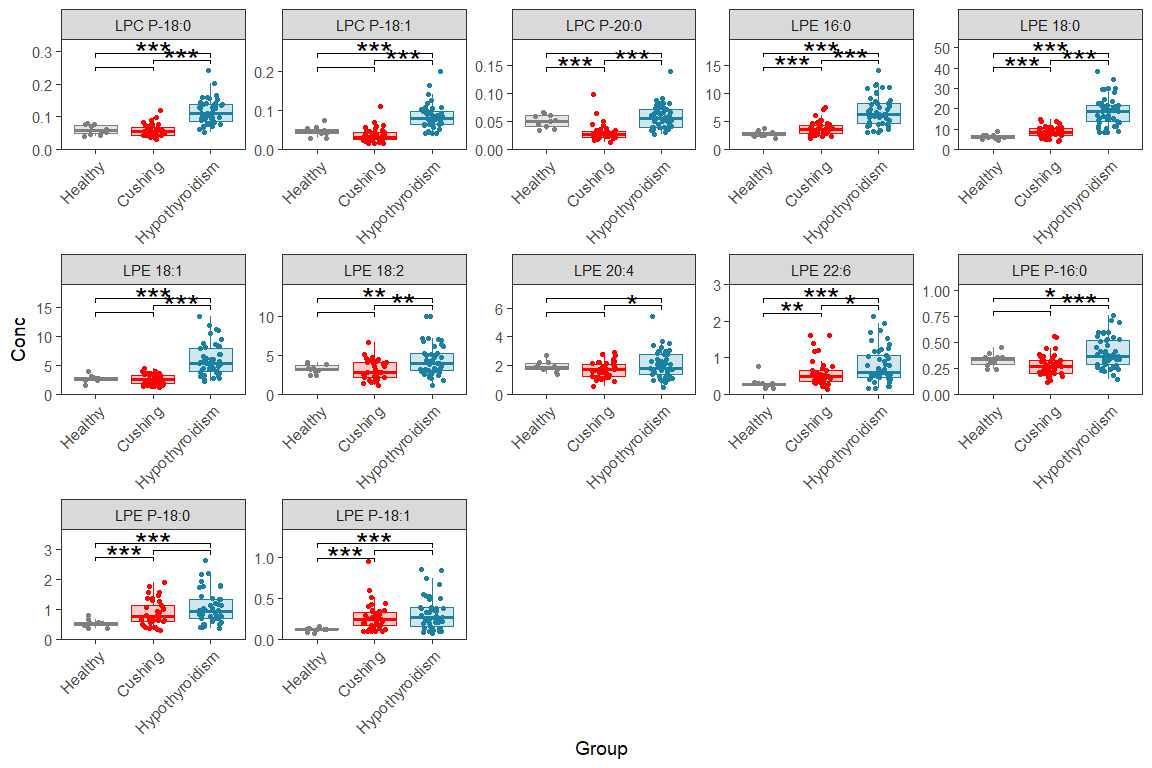
\includegraphics[width=18.75in,height=\textheight]{./dotplot_lipidomics_files/figure-pdf/plot-2-3.pdf}

}

\end{figure}

\hypertarget{save-multi-page-plot-a-pdf-1}{%
\section{Save multi-page plot a
PDF}\label{save-multi-page-plot-a-pdf-1}}

\begin{Shaded}
\begin{Highlighting}[]
\FunctionTok{pdf}\NormalTok{(}\AttributeTok{file =} \StringTok{"myplot.pdf"}\NormalTok{, }\AttributeTok{onefile =} \ConstantTok{TRUE}\NormalTok{, }\AttributeTok{paper =} \StringTok{"A4r"}\NormalTok{, }\AttributeTok{width =} \DecValTok{11}\NormalTok{)}
\NormalTok{my\_plots}\SpecialCharTok{$}\NormalTok{plt}
\FunctionTok{dev.off}\NormalTok{()}
\end{Highlighting}
\end{Shaded}

\hypertarget{regressions-for-many-lipids}{%
\chapter{Regressions for many
lipids}\label{regressions-for-many-lipids}}

\hypertarget{libraries-4}{%
\section{Libraries}\label{libraries-4}}

\begin{Shaded}
\begin{Highlighting}[]
\FunctionTok{library}\NormalTok{(here)}
\FunctionTok{library}\NormalTok{(tidyverse)}
\FunctionTok{library}\NormalTok{(broom)}
\FunctionTok{library}\NormalTok{(ggpmisc)}
\end{Highlighting}
\end{Shaded}

\hypertarget{overview-lm-and-broom-package}{%
\section{Overview lm and `broom'
package}\label{overview-lm-and-broom-package}}

\begin{Shaded}
\begin{Highlighting}[]
\NormalTok{d\_test }\OtherTok{\textless{}{-}} \FunctionTok{tibble}\NormalTok{(}\AttributeTok{InjVol =} \FunctionTok{c}\NormalTok{(}\DecValTok{0}\NormalTok{,}\FloatTok{0.2}\NormalTok{, }\FloatTok{0.4}\NormalTok{, }\FloatTok{0.6}\NormalTok{, }\FloatTok{0.8}\NormalTok{,}\DecValTok{1}\NormalTok{),}
                  \AttributeTok{Response  =} \FunctionTok{c}\NormalTok{(}\DecValTok{12}\NormalTok{, }\DecValTok{23}\NormalTok{, }\DecValTok{34}\NormalTok{,}\DecValTok{44}\NormalTok{, }\DecValTok{89}\NormalTok{, }\DecValTok{101}\NormalTok{)) }
                 
\NormalTok{d\_test}
\end{Highlighting}
\end{Shaded}

\begin{verbatim}
#> # A tibble: 6 x 2
#>   InjVol Response
#>    <dbl>    <dbl>
#> 1    0         12
#> 2    0.2       23
#> 3    0.4       34
#> 4    0.6       44
#> 5    0.8       89
#> 6    1        101
\end{verbatim}

\begin{Shaded}
\begin{Highlighting}[]
\CommentTok{\# Linear model}
\NormalTok{model }\OtherTok{\textless{}{-}} \FunctionTok{lm}\NormalTok{(}\AttributeTok{formula =}\NormalTok{ Response }\SpecialCharTok{\textasciitilde{}}\NormalTok{ InjVol, }\AttributeTok{data =}\NormalTok{ d\_test)}

\CommentTok{\# Get result summary}
\FunctionTok{summary}\NormalTok{(model)}
\end{Highlighting}
\end{Shaded}

\begin{verbatim}
#> 
#> Call:
#> lm(formula = Response ~ InjVol, data = d_test)
#> 
#> Residuals:
#>        1        2        3        4        5        6 
#>   8.1429   0.4857  -7.1714 -15.8286  10.5143   3.8571 
#> 
#> Coefficients:
#>             Estimate Std. Error t value Pr(>|t|)   
#> (Intercept)    3.857      8.043   0.480  0.65656   
#> InjVol        93.286     13.282   7.024  0.00216 **
#> ---
#> Signif. codes:  0 '***' 0.001 '**' 0.01 '*' 0.05 '.' 0.1 ' ' 1
#> 
#> Residual standard error: 11.11 on 4 degrees of freedom
#> Multiple R-squared:  0.925,  Adjusted R-squared:  0.9062 
#> F-statistic: 49.33 on 1 and 4 DF,  p-value: 0.002165
\end{verbatim}

\begin{Shaded}
\begin{Highlighting}[]
\CommentTok{\# Get r\^{}2 only}
\FunctionTok{summary}\NormalTok{(model)}\SpecialCharTok{$}\NormalTok{r.squared}
\end{Highlighting}
\end{Shaded}

\begin{verbatim}
#> [1] 0.9249954
\end{verbatim}

\begin{Shaded}
\begin{Highlighting}[]
\CommentTok{\# Using broom functions to summarize model results into a table}
\NormalTok{broom}\SpecialCharTok{::}\FunctionTok{glance}\NormalTok{(model) }
\end{Highlighting}
\end{Shaded}

\begin{verbatim}
#> # A tibble: 1 x 12
#>   r.squared adj.r.squared sigma statistic p.value    df logLik   AIC   BIC
#>       <dbl>         <dbl> <dbl>     <dbl>   <dbl> <dbl>  <dbl> <dbl> <dbl>
#> 1     0.925         0.906  11.1      49.3 0.00216     1  -21.7  49.5  48.9
#> # ... with 3 more variables: deviance <dbl>, df.residual <int>, nobs <int>
\end{verbatim}

\begin{Shaded}
\begin{Highlighting}[]
\NormalTok{broom}\SpecialCharTok{::}\FunctionTok{tidy}\NormalTok{(model) }
\end{Highlighting}
\end{Shaded}

\begin{verbatim}
#> # A tibble: 2 x 5
#>   term        estimate std.error statistic p.value
#>   <chr>          <dbl>     <dbl>     <dbl>   <dbl>
#> 1 (Intercept)     3.86      8.04     0.480 0.657  
#> 2 InjVol         93.3      13.3      7.02  0.00216
\end{verbatim}

\hypertarget{import-datasets-1}{%
\section{Import Datasets}\label{import-datasets-1}}

\begin{Shaded}
\begin{Highlighting}[]
\NormalTok{d\_orig }\OtherTok{\textless{}{-}} \FunctionTok{read\_csv}\NormalTok{(}\FunctionTok{here}\NormalTok{(}\StringTok{"data/Testdata\_Lipidomics\_flat\_wide\_annotated\_V1.csv"}\NormalTok{))}
\end{Highlighting}
\end{Shaded}

\hypertarget{prepare-data-1}{%
\section{Prepare Data}\label{prepare-data-1}}

\begin{Shaded}
\begin{Highlighting}[]
\CommentTok{\# Convert to long format}

\CommentTok{\# Convert to long format}
\NormalTok{d\_long }\OtherTok{\textless{}{-}}\NormalTok{ d\_orig }\SpecialCharTok{|\textgreater{}} 
  \FunctionTok{pivot\_longer}\NormalTok{(}\AttributeTok{cols =} \SpecialCharTok{{-}}\NormalTok{DataFileName}\SpecialCharTok{:{-}}\NormalTok{InjVol, }
               \AttributeTok{names\_to =} \StringTok{"Lipid"}\NormalTok{ , }
               \AttributeTok{values\_to =} \StringTok{"Area"}\NormalTok{)}

\CommentTok{\# Get a table with RQCs only and sort by Lipid}
\NormalTok{d\_rqc }\OtherTok{\textless{}{-}}\NormalTok{ d\_long }\SpecialCharTok{|\textgreater{}} 
  \FunctionTok{filter}\NormalTok{(QCtype }\SpecialCharTok{==} \StringTok{"RQC"}\NormalTok{) }\SpecialCharTok{|\textgreater{}} 
  \FunctionTok{arrange}\NormalTok{(Lipid)}
\end{Highlighting}
\end{Shaded}

\hypertarget{run-regression-for-each-lipid}{%
\section{Run regression for each
lipid}\label{run-regression-for-each-lipid}}

In this example a logistic regression is used. The output of
\texttt{glm()} is converted to a tidy table using the
\texttt{broom::tidy()} function.

\begin{Shaded}
\begin{Highlighting}[]
\NormalTok{model }\OtherTok{\textless{}{-}} \FunctionTok{as.formula}\NormalTok{(}\StringTok{"Area \textasciitilde{} InjVol"}\NormalTok{)}

\NormalTok{d\_res }\OtherTok{\textless{}{-}}\NormalTok{ d\_rqc }\SpecialCharTok{\%\textgreater{}\%}
  \FunctionTok{group\_by}\NormalTok{(Lipid) }\SpecialCharTok{\%\textgreater{}\%}
  \FunctionTok{nest}\NormalTok{() }\SpecialCharTok{\%\textgreater{}\%}
  \FunctionTok{mutate}\NormalTok{(}
    \AttributeTok{models =} \FunctionTok{map}\NormalTok{(data, }\ControlFlowTok{function}\NormalTok{(x) }\FunctionTok{lm}\NormalTok{(model, }\AttributeTok{data =}\NormalTok{ x)), }
    \CommentTok{\#mandel = map(data, \textbackslash{}(x) DCVtestkit::calculate\_mandel(x, "InjVol", "Area")),}
    \CommentTok{\#ppa = map(data, \textbackslash{}(x) DCVtestkit::calculate\_pra\_linear(x, "InjVol", "Area")),}
    \AttributeTok{tidy =} \FunctionTok{map}\NormalTok{(models, }\ControlFlowTok{function}\NormalTok{(x) broom}\SpecialCharTok{::}\FunctionTok{glance}\NormalTok{(x))) }\SpecialCharTok{|\textgreater{}} 
  \FunctionTok{unnest}\NormalTok{(}\FunctionTok{c}\NormalTok{(tidy)) }\SpecialCharTok{|\textgreater{}} 
\NormalTok{  dplyr}\SpecialCharTok{::}\FunctionTok{select}\NormalTok{(}\SpecialCharTok{{-}}\NormalTok{data, }\SpecialCharTok{{-}}\NormalTok{models)}

\CommentTok{\# Fix DCVtestkit::calculate\_pra\_linear currently returning a list instead vector}
\CommentTok{\# d\_res$ppa \textless{}{-} unlist(d\_res$ppa)}
\end{Highlighting}
\end{Shaded}

The results contain the combined estimates, errors, and \emph{P} values
for each term for each lipid species.

\begin{longtable}[]{@{}
  >{\raggedright\arraybackslash}p{(\columnwidth - 24\tabcolsep) * \real{0.1333}}
  >{\raggedleft\arraybackslash}p{(\columnwidth - 24\tabcolsep) * \real{0.0741}}
  >{\raggedleft\arraybackslash}p{(\columnwidth - 24\tabcolsep) * \real{0.1037}}
  >{\raggedleft\arraybackslash}p{(\columnwidth - 24\tabcolsep) * \real{0.0963}}
  >{\raggedleft\arraybackslash}p{(\columnwidth - 24\tabcolsep) * \real{0.0741}}
  >{\raggedleft\arraybackslash}p{(\columnwidth - 24\tabcolsep) * \real{0.0667}}
  >{\raggedleft\arraybackslash}p{(\columnwidth - 24\tabcolsep) * \real{0.0222}}
  >{\raggedleft\arraybackslash}p{(\columnwidth - 24\tabcolsep) * \real{0.0741}}
  >{\raggedleft\arraybackslash}p{(\columnwidth - 24\tabcolsep) * \real{0.0667}}
  >{\raggedleft\arraybackslash}p{(\columnwidth - 24\tabcolsep) * \real{0.0667}}
  >{\raggedleft\arraybackslash}p{(\columnwidth - 24\tabcolsep) * \real{0.0963}}
  >{\raggedleft\arraybackslash}p{(\columnwidth - 24\tabcolsep) * \real{0.0889}}
  >{\raggedleft\arraybackslash}p{(\columnwidth - 24\tabcolsep) * \real{0.0370}}@{}}
\toprule()
\begin{minipage}[b]{\linewidth}\raggedright
Lipid
\end{minipage} & \begin{minipage}[b]{\linewidth}\raggedleft
r.squared
\end{minipage} & \begin{minipage}[b]{\linewidth}\raggedleft
adj.r.squared
\end{minipage} & \begin{minipage}[b]{\linewidth}\raggedleft
sigma
\end{minipage} & \begin{minipage}[b]{\linewidth}\raggedleft
statistic
\end{minipage} & \begin{minipage}[b]{\linewidth}\raggedleft
p.value
\end{minipage} & \begin{minipage}[b]{\linewidth}\raggedleft
df
\end{minipage} & \begin{minipage}[b]{\linewidth}\raggedleft
logLik
\end{minipage} & \begin{minipage}[b]{\linewidth}\raggedleft
AIC
\end{minipage} & \begin{minipage}[b]{\linewidth}\raggedleft
BIC
\end{minipage} & \begin{minipage}[b]{\linewidth}\raggedleft
deviance
\end{minipage} & \begin{minipage}[b]{\linewidth}\raggedleft
df.residual
\end{minipage} & \begin{minipage}[b]{\linewidth}\raggedleft
nobs
\end{minipage} \\
\midrule()
\endhead
CE 16:0 & 0.626274 & 0.602917 & 44054.0359 & 26.81215 & 0.000092 & 1 &
-216.9579 & 439.9159 & 442.5870 & 3.105213e+10 & 16 & 18 \\
CE 16:1 & 0.834197 & 0.823834 & 8622.1216 & 80.50006 & 0.000000 & 1 &
-187.5984 & 381.1968 & 383.8679 & 1.189456e+09 & 16 & 18 \\
CE 16:2 & 0.609873 & 0.585490 & 585.7358 & 25.01226 & 0.000131 & 1 &
-139.1925 & 284.3850 & 287.0561 & 5.489383e+06 & 16 & 18 \\
CE 17:0 & 0.900585 & 0.894371 & 1178.0217 & 144.94082 & 0.000000 & 1 &
-151.7695 & 309.5390 & 312.2101 & 2.220376e+07 & 16 & 18 \\
CE 17:1 & 0.945373 & 0.941959 & 1914.1239 & 276.89543 & 0.000000 & 1 &
-160.5071 & 327.0142 & 329.6854 & 5.862192e+07 & 16 & 18 \\
CE 18:0 & 0.952998 & 0.950061 & 8748.1092 & 324.41314 & 0.000000 & 1 &
-187.8595 & 381.7190 & 384.3902 & 1.224471e+09 & 16 & 18 \\
CE 18:1 & 0.944273 & 0.940791 & 522750.3432 & 271.11631 & 0.000000 & 1 &
-261.4843 & 528.9686 & 531.6397 & 4.372287e+12 & 16 & 18 \\
CE 18:1 d7 (ISTD) & 0.922337 & 0.917483 & 60313.2929 & 190.01887 &
0.000000 & 1 & -222.6124 & 451.2248 & 453.8959 & 5.820309e+10 & 16 &
18 \\
CE 18:2 & 0.950589 & 0.947501 & 2583852.0035 & 307.81495 & 0.000000 & 1
& -290.2471 & 586.4942 & 589.1653 & 1.068207e+14 & 16 & 18 \\
CE 18:3 & 0.767452 & 0.752918 & 88635.9222 & 52.80302 & 0.000002 & 1 &
-229.5421 & 465.0842 & 467.7553 & 1.257012e+11 & 16 & 18 \\
\bottomrule()
\end{longtable}

\hypertarget{multivariate-regression}{%
\chapter{Multivariate Regression}\label{multivariate-regression}}

\hypertarget{libraries-5}{%
\section{Libraries}\label{libraries-5}}

\begin{Shaded}
\begin{Highlighting}[]
\FunctionTok{library}\NormalTok{(here)}
\FunctionTok{library}\NormalTok{(tidyverse)}
\FunctionTok{library}\NormalTok{(SLINGtools)}
\FunctionTok{library}\NormalTok{(broom)}
\FunctionTok{library}\NormalTok{(ggrepel)}
\end{Highlighting}
\end{Shaded}

\hypertarget{import-datasets-2}{%
\section{Import Datasets}\label{import-datasets-2}}

\begin{Shaded}
\begin{Highlighting}[]
\NormalTok{d\_meta }\OtherTok{\textless{}{-}} \FunctionTok{read\_csv}\NormalTok{(}\FunctionTok{here}\NormalTok{(}\StringTok{"data/ISLS10\_Part2\_metadata.csv"}\NormalTok{))}
\NormalTok{d\_wide }\OtherTok{\textless{}{-}} \FunctionTok{read\_csv}\NormalTok{(}\FunctionTok{here}\NormalTok{(}\StringTok{"data/ISLS10\_Part2\_lipidomics\_curated.csv"}\NormalTok{))}
\end{Highlighting}
\end{Shaded}

\hypertarget{prepare-data-2}{%
\section{Prepare Data}\label{prepare-data-2}}

\begin{Shaded}
\begin{Highlighting}[]
\CommentTok{\# Convert to long format}
\NormalTok{d\_long }\OtherTok{\textless{}{-}}\NormalTok{ d\_wide }\SpecialCharTok{|\textgreater{}}
  \FunctionTok{pivot\_longer}\NormalTok{(}\AttributeTok{cols =} \SpecialCharTok{{-}}\NormalTok{ID, }\AttributeTok{names\_to =} \StringTok{"Compound"}\NormalTok{ , }\AttributeTok{values\_to =} \StringTok{"Conc"}\NormalTok{)}

\CommentTok{\# Combine data and metadata}
\NormalTok{d\_full }\OtherTok{\textless{}{-}}\NormalTok{ d\_meta }\SpecialCharTok{|\textgreater{}} \FunctionTok{left\_join}\NormalTok{(d\_long, }\AttributeTok{by =} \StringTok{"ID"}\NormalTok{)}

\CommentTok{\# log{-}transform and scale (z{-}score) data}
\NormalTok{d\_full }\OtherTok{\textless{}{-}}\NormalTok{ d\_full }\SpecialCharTok{|\textgreater{}}
  \FunctionTok{group\_by}\NormalTok{(Compound) }\SpecialCharTok{|\textgreater{}}
  \FunctionTok{mutate}\NormalTok{(}\AttributeTok{Conc\_log =} \FunctionTok{log2}\NormalTok{(Conc),}
         \AttributeTok{Conc\_logz =} \FunctionTok{as.numeric}\NormalTok{(}\FunctionTok{scale}\NormalTok{(Conc\_log)))}
\end{Highlighting}
\end{Shaded}

\hypertarget{run-regression-for-each-lipid-1}{%
\section{Run regression for each
lipid}\label{run-regression-for-each-lipid-1}}

In this example a logistic regression is used. The output of
\texttt{glm()} is converted to a tidy table using the
\texttt{broom::tidy()} function.

\begin{Shaded}
\begin{Highlighting}[]
\NormalTok{model }\OtherTok{\textless{}{-}} \FunctionTok{as.formula}\NormalTok{(}\StringTok{"DM \textasciitilde{} Age + Gender + BMI + HbA1c + }
\StringTok{                    SBP + HDL + LDL + TG + Conc\_logz"}\NormalTok{)}

\NormalTok{d\_res }\OtherTok{\textless{}{-}}\NormalTok{ d\_full }\SpecialCharTok{\%\textgreater{}\%}
  \FunctionTok{group\_by}\NormalTok{(Compound) }\SpecialCharTok{\%\textgreater{}\%}
  \FunctionTok{nest}\NormalTok{() }\SpecialCharTok{\%\textgreater{}\%}
  \FunctionTok{mutate}\NormalTok{(}
    \AttributeTok{models =} \FunctionTok{map}\NormalTok{(data, }\ControlFlowTok{function}\NormalTok{(x) }\FunctionTok{glm}\NormalTok{(model, }\AttributeTok{data =}\NormalTok{ x, }\AttributeTok{family =} \StringTok{"binomial"}\NormalTok{)), }
    \AttributeTok{tidy =} \FunctionTok{map}\NormalTok{(models, }\ControlFlowTok{function}\NormalTok{(x) broom}\SpecialCharTok{::}\FunctionTok{tidy}\NormalTok{(x))) }\SpecialCharTok{|\textgreater{}} 
  \FunctionTok{unnest}\NormalTok{(tidy) }\SpecialCharTok{|\textgreater{}} 
\NormalTok{  dplyr}\SpecialCharTok{::}\FunctionTok{select}\NormalTok{(}\SpecialCharTok{{-}}\NormalTok{data, }\SpecialCharTok{{-}}\NormalTok{models)}
\end{Highlighting}
\end{Shaded}

The results contain the combined estimates, errors, and \emph{P} values
for each term for each lipid species.

\begin{longtable}[]{@{}
  >{\raggedright\arraybackslash}p{(\columnwidth - 10\tabcolsep) * \real{0.2206}}
  >{\raggedright\arraybackslash}p{(\columnwidth - 10\tabcolsep) * \real{0.1765}}
  >{\raggedleft\arraybackslash}p{(\columnwidth - 10\tabcolsep) * \real{0.1618}}
  >{\raggedleft\arraybackslash}p{(\columnwidth - 10\tabcolsep) * \real{0.1471}}
  >{\raggedleft\arraybackslash}p{(\columnwidth - 10\tabcolsep) * \real{0.1618}}
  >{\raggedleft\arraybackslash}p{(\columnwidth - 10\tabcolsep) * \real{0.1324}}@{}}
\toprule()
\begin{minipage}[b]{\linewidth}\raggedright
Compound
\end{minipage} & \begin{minipage}[b]{\linewidth}\raggedright
term
\end{minipage} & \begin{minipage}[b]{\linewidth}\raggedleft
estimate
\end{minipage} & \begin{minipage}[b]{\linewidth}\raggedleft
std.error
\end{minipage} & \begin{minipage}[b]{\linewidth}\raggedleft
statistic
\end{minipage} & \begin{minipage}[b]{\linewidth}\raggedleft
p.value
\end{minipage} \\
\midrule()
\endhead
Cer d16:1/16:0 & (Intercept) & -20.955219 & 1.886056 & -11.110601 &
0.000000 \\
Cer d16:1/16:0 & Age & 0.032885 & 0.010896 & 3.017987 & 0.002545 \\
Cer d16:1/16:0 & Gender & 0.593323 & 0.217179 & 2.731950 & 0.006296 \\
Cer d16:1/16:0 & BMI & 0.129663 & 0.027600 & 4.698024 & 0.000003 \\
Cer d16:1/16:0 & HbA1c & 2.041818 & 0.281859 & 7.244102 & 0.000000 \\
Cer d16:1/16:0 & SBP & 0.017569 & 0.005370 & 3.271562 & 0.001070 \\
Cer d16:1/16:0 & HDL & -0.725890 & 0.368385 & -1.970465 & 0.048785 \\
Cer d16:1/16:0 & LDL & -0.247450 & 0.128041 & -1.932579 & 0.053288 \\
Cer d16:1/16:0 & TG & 0.402731 & 0.142030 & 2.835530 & 0.004575 \\
Cer d16:1/16:0 & Conc\_logz & 0.197851 & 0.113746 & 1.739413 &
0.081962 \\
\bottomrule()
\end{longtable}

To get the effects and \emph{P} values for the lipids we filter for the
term \texttt{Conc\_logz}. We futhermore get the adjusted \emph{P} values
(FDR).

\begin{Shaded}
\begin{Highlighting}[]
\NormalTok{d\_res\_lipids }\OtherTok{\textless{}{-}}\NormalTok{ d\_res }\SpecialCharTok{|\textgreater{}} 
   \FunctionTok{filter}\NormalTok{(term }\SpecialCharTok{==} \StringTok{"Conc\_logz"}\NormalTok{) }\SpecialCharTok{|\textgreater{}} 
   \FunctionTok{mutate}\NormalTok{(}\AttributeTok{FDR =} \FunctionTok{p.adjust}\NormalTok{(p.value, }\AttributeTok{method =} \StringTok{"fdr"}\NormalTok{)) }\SpecialCharTok{|\textgreater{}} 
   \FunctionTok{arrange}\NormalTok{(FDR)}
\end{Highlighting}
\end{Shaded}

\begin{longtable}[]{@{}
  >{\raggedright\arraybackslash}p{(\columnwidth - 12\tabcolsep) * \real{0.2468}}
  >{\raggedright\arraybackslash}p{(\columnwidth - 12\tabcolsep) * \real{0.1299}}
  >{\raggedleft\arraybackslash}p{(\columnwidth - 12\tabcolsep) * \real{0.1299}}
  >{\raggedleft\arraybackslash}p{(\columnwidth - 12\tabcolsep) * \real{0.1299}}
  >{\raggedleft\arraybackslash}p{(\columnwidth - 12\tabcolsep) * \real{0.1299}}
  >{\raggedleft\arraybackslash}p{(\columnwidth - 12\tabcolsep) * \real{0.1169}}
  >{\raggedleft\arraybackslash}p{(\columnwidth - 12\tabcolsep) * \real{0.1169}}@{}}
\toprule()
\begin{minipage}[b]{\linewidth}\raggedright
Compound
\end{minipage} & \begin{minipage}[b]{\linewidth}\raggedright
term
\end{minipage} & \begin{minipage}[b]{\linewidth}\raggedleft
estimate
\end{minipage} & \begin{minipage}[b]{\linewidth}\raggedleft
std.error
\end{minipage} & \begin{minipage}[b]{\linewidth}\raggedleft
statistic
\end{minipage} & \begin{minipage}[b]{\linewidth}\raggedleft
p.value
\end{minipage} & \begin{minipage}[b]{\linewidth}\raggedleft
FDR
\end{minipage} \\
\midrule()
\endhead
SM d16:1/18:0 & Conc\_logz & 0.408832 & 0.119650 & 3.416896 & 0.000633 &
0.000633 \\
SM d18:1/18:0 & Conc\_logz & 0.325500 & 0.105045 & 3.098661 & 0.001944 &
0.001944 \\
Cer d18:0/18:0 & Conc\_logz & 0.427791 & 0.139298 & 3.071052 & 0.002133
& 0.002133 \\
Hex1Cer d18:2/25:0 & Conc\_logz & -0.255110 & 0.092979 & -2.743742 &
0.006074 & 0.006074 \\
Cer d18:1/18:0 & Conc\_logz & 0.316480 & 0.119278 & 2.653288 & 0.007971
& 0.007971 \\
SM d18:1/20:0 & Conc\_logz & 0.282201 & 0.106676 & 2.645399 & 0.008159 &
0.008159 \\
\bottomrule()
\end{longtable}

\hypertarget{forest-plot}{%
\section{Forest Plot}\label{forest-plot}}

Prepare data for the plot: get lipid class from lipid names, join it to
the data frame, calculate FDR, get upper/lower errors, and set
``significant specie''

\begin{Shaded}
\begin{Highlighting}[]
\CommentTok{\# lipid annotation}
\NormalTok{d\_lipid\_annot }\OtherTok{\textless{}{-}}\NormalTok{ d\_res\_lipids }\SpecialCharTok{|\textgreater{}}
  \FunctionTok{select}\NormalTok{(Compound) }\SpecialCharTok{|\textgreater{}}  
  \FunctionTok{separate}\NormalTok{(Compound, }
           \AttributeTok{into =} \FunctionTok{c}\NormalTok{(}\StringTok{"lipid\_class"}\NormalTok{, }\StringTok{"fa\_chain"}\NormalTok{), }
           \AttributeTok{remove =} \ConstantTok{FALSE}\NormalTok{, }
           \AttributeTok{extra =} \StringTok{"drop"}\NormalTok{,}
           \AttributeTok{fill =} \StringTok{"right"}\NormalTok{,  }
           \AttributeTok{sep =} \StringTok{"/"}\NormalTok{ )}

\NormalTok{d\_plot }\OtherTok{\textless{}{-}}\NormalTok{ d\_res\_lipids }\SpecialCharTok{|\textgreater{}} 
  \FunctionTok{full\_join}\NormalTok{(d\_lipid\_annot, }\AttributeTok{by =} \StringTok{"Compound"}\NormalTok{) }\SpecialCharTok{|\textgreater{}} 
  \FunctionTok{mutate}\NormalTok{(}
    \AttributeTok{est\_low =}\NormalTok{ estimate }\SpecialCharTok{{-}}\NormalTok{ std.error,}
    \AttributeTok{est\_high =}\NormalTok{ estimate }\SpecialCharTok{+}\NormalTok{ std.error, }
    \AttributeTok{signif =}\NormalTok{ FDR }\SpecialCharTok{\textless{}} \FloatTok{0.05}\NormalTok{,}
    \AttributeTok{label =} \FunctionTok{if\_else}\NormalTok{(signif, fa\_chain, }\StringTok{""}\NormalTok{)) }\SpecialCharTok{|\textgreater{}} 
  \FunctionTok{arrange}\NormalTok{(signif)}
\end{Highlighting}
\end{Shaded}

Plot estimates of all lipid species, grouped by lipid class,
highlighting significant species in red and label them by the FA chain.

\begin{Shaded}
\begin{Highlighting}[]
\FunctionTok{ggplot}\NormalTok{(d\_plot, }\FunctionTok{aes}\NormalTok{(}\AttributeTok{x =}\NormalTok{ lipid\_class, }\AttributeTok{y =}\NormalTok{ estimate,}\AttributeTok{color =}\NormalTok{ signif, }\AttributeTok{label =}\NormalTok{ label)) }\SpecialCharTok{+}
  \FunctionTok{geom\_hline}\NormalTok{(}\AttributeTok{yintercept =} \DecValTok{0}\NormalTok{) }\SpecialCharTok{+}
  \FunctionTok{geom\_pointrange}\NormalTok{(}\FunctionTok{aes}\NormalTok{(}\AttributeTok{ymin =}\NormalTok{ est\_low, }\AttributeTok{ymax =}\NormalTok{ est\_high, }\AttributeTok{alpha =}\NormalTok{ signif),}
                  \AttributeTok{size =} \FloatTok{0.5}\NormalTok{,}
                  \AttributeTok{position =} \FunctionTok{position\_jitter}\NormalTok{(}\AttributeTok{width =}\NormalTok{ .}\DecValTok{3}\NormalTok{, }\AttributeTok{height =} \DecValTok{0}\NormalTok{)) }\SpecialCharTok{+}
  \FunctionTok{coord\_flip}\NormalTok{() }\SpecialCharTok{+}
  \FunctionTok{scale\_color\_manual}\NormalTok{(}\AttributeTok{values =} \FunctionTok{c}\NormalTok{(}\StringTok{"FALSE"} \OtherTok{=} \StringTok{"grey70"}\NormalTok{, }\StringTok{"TRUE"} \OtherTok{=} \StringTok{"red"}\NormalTok{)) }\SpecialCharTok{+}
  \FunctionTok{scale\_alpha\_manual}\NormalTok{(}\AttributeTok{values =} \FunctionTok{c}\NormalTok{(}\StringTok{"FALSE"} \OtherTok{=} \FloatTok{0.3}\NormalTok{, }\StringTok{"TRUE"} \OtherTok{=} \DecValTok{1}\NormalTok{)) }\SpecialCharTok{+}
\NormalTok{  ggrepel}\SpecialCharTok{::}\FunctionTok{geom\_text\_repel}\NormalTok{(}
    \FunctionTok{aes}\NormalTok{(}\AttributeTok{y =}\NormalTok{ estimate),}
    \AttributeTok{size =} \DecValTok{2}\NormalTok{,}
    \AttributeTok{max.overlaps =} \DecValTok{5}\NormalTok{,}
    \AttributeTok{point.padding =}\NormalTok{ .}\DecValTok{7}
\NormalTok{  ) }\SpecialCharTok{+}
  \FunctionTok{theme\_bw}\NormalTok{() }\SpecialCharTok{+} 
  \FunctionTok{theme}\NormalTok{(}\AttributeTok{legend.position=}\StringTok{"none"}\NormalTok{)}
\end{Highlighting}
\end{Shaded}

\begin{figure}[H]

{\centering 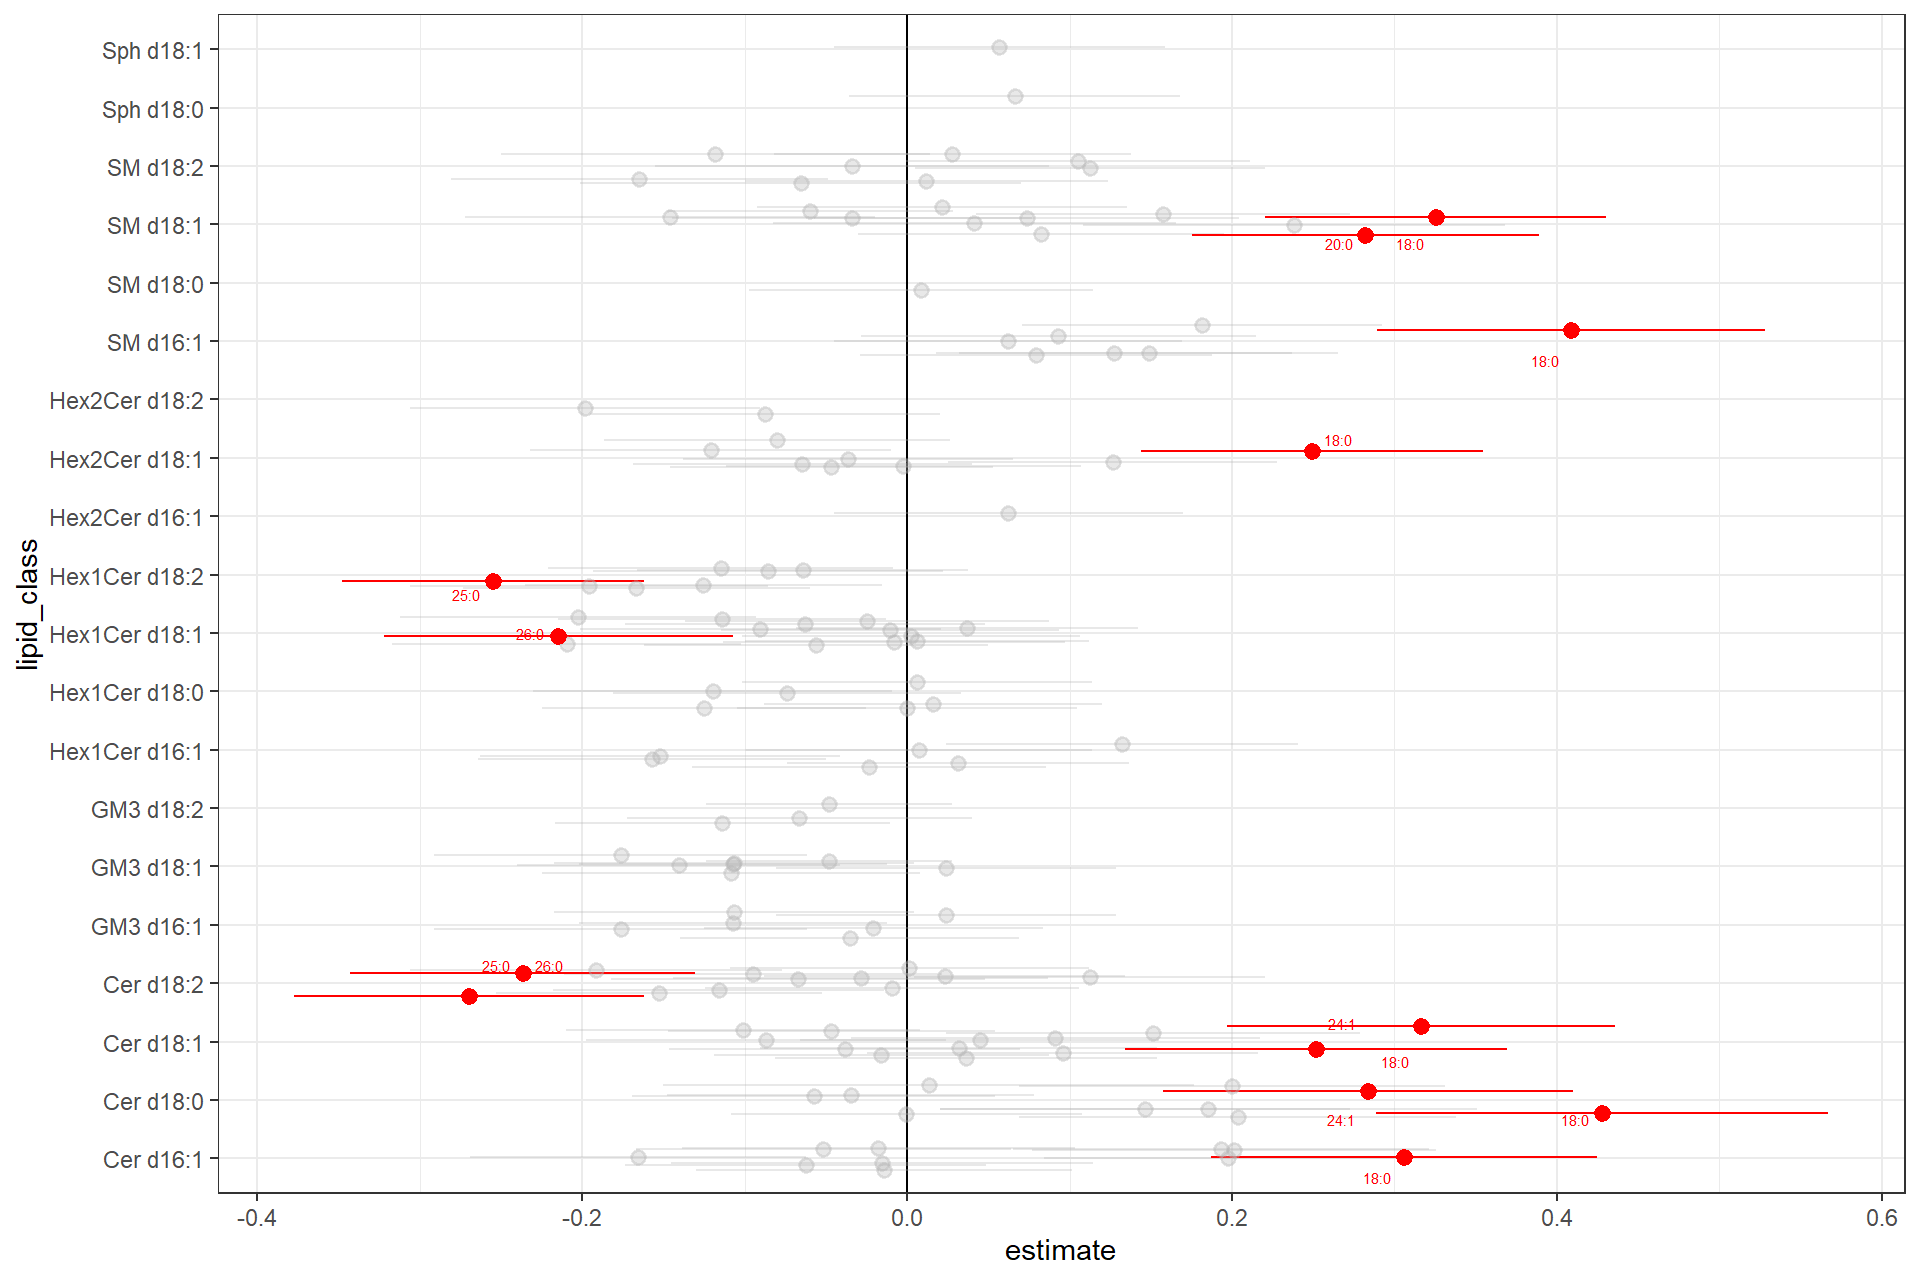
\includegraphics[width=31.25in,height=\textheight]{./multiple_models_files/figure-pdf/forestplot-1.pdf}

}

\caption{Figure 1. Forest plot of logistic regression (DM
\textasciitilde{} Age + Gender + BMI + HbA1c + SBP + HDL + LDL + TG +
Lipid). Species with FDR \textgreater{} 0.05 are highlighted in red.}

\end{figure}

\hypertarget{read-ms-datasets-into-r}{%
\chapter{Read MS datasets into R}\label{read-ms-datasets-into-r}}

Pre-processed MS datasets refers to data exported from MS rawdata
processing software, such as Agilent MassHunter, Sciex Multiquant, and
open-source tools as MRMkit and Skyline. These datasets usually contain
peak/signal intensities and associated data such as retention time,
FWHM, as well as information about the sample.

The R package \href{https://github.com/SLINGhub/SLINGtools}{SLINGtools}
provided helper functions to import data files obtained from different
tools.

\hypertarget{import-peak-areas-from-agilent-masshunter-csv-file}{%
\section{Import peak areas from Agilent MassHunter CSV
file}\label{import-peak-areas-from-agilent-masshunter-csv-file}}

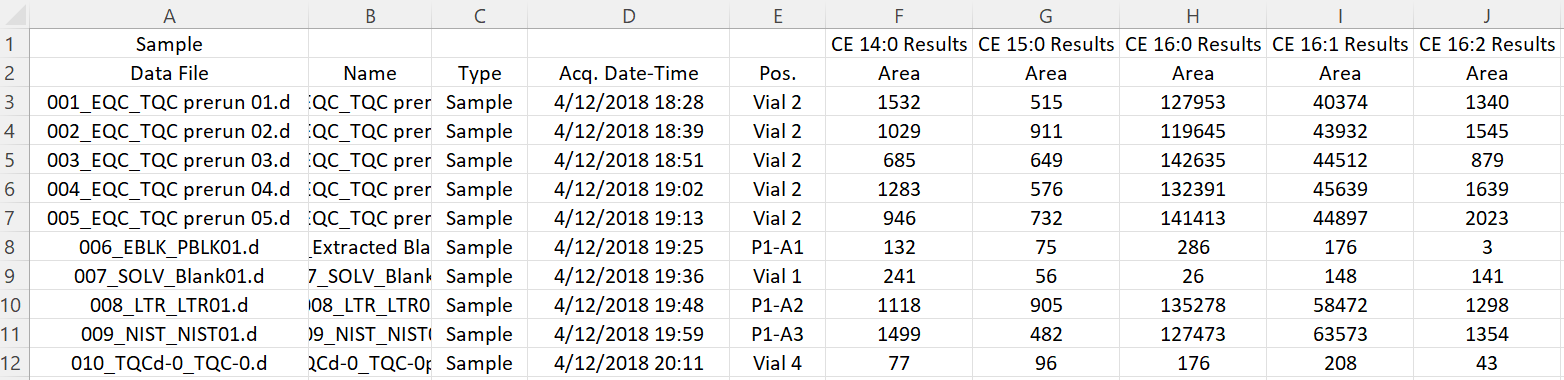
\includegraphics{./images/paste-B702CE09.png}

\begin{Shaded}
\begin{Highlighting}[]
\FunctionTok{library}\NormalTok{(SLINGtools)}
\NormalTok{data\_file\_path }\OtherTok{\textless{}{-}}\NormalTok{ here}\SpecialCharTok{::}\FunctionTok{here}\NormalTok{(}\StringTok{"data/Testdata\_Lipidomics\_MHQuant\_Detailed\_V2.csv"}\NormalTok{)}
\NormalTok{d\_wide }\OtherTok{\textless{}{-}}\NormalTok{ SLINGtools}\SpecialCharTok{::}\FunctionTok{read\_MassHunterCSV\_wide}\NormalTok{(data\_file\_path, }\AttributeTok{field =} \StringTok{"Area"}\NormalTok{)}
\end{Highlighting}
\end{Shaded}

\begin{verbatim}
Reading 'Testdata_Lipidomics_MHQuant_Detailed_V2.csv' ... 

indexing Testdata_Lipidomics_MHQuant_Detailed_V2.csv [======] 2.15GB/s, eta:  0s
                                                                                
Imported  215 samples with 428 transitions 
\end{verbatim}

\begin{Shaded}
\begin{Highlighting}[]
\FunctionTok{print}\NormalTok{(d\_wide)}
\end{Highlighting}
\end{Shaded}

\begin{verbatim}
# A tibble: 215 x 432
   DataFileName  AcqTimeStamp        SampleType VialPosition `CE 14:0` `CE 15:0`
   <chr>         <dttm>              <chr>      <chr>            <dbl>     <dbl>
 1 001_EQC_TQC ~ 2018-04-12 18:28:00 EQC        Vial 2            1532       515
 2 002_EQC_TQC ~ 2018-04-12 18:39:00 EQC        Vial 2            1029       911
 3 003_EQC_TQC ~ 2018-04-12 18:51:00 EQC        Vial 2             685       649
 4 004_EQC_TQC ~ 2018-04-12 19:02:00 EQC        Vial 2            1283       576
 5 005_EQC_TQC ~ 2018-04-12 19:13:00 EQC        Vial 2             946       732
 6 006_EBLK_Ext~ 2018-04-12 19:25:00 PBLK       P1-A1              132        75
 7 007_SOLV_Bla~ 2018-04-12 19:36:00 SBLK       Vial 1             241        56
 8 008_LTR_LTR0~ 2018-04-12 19:48:00 LTR        P1-A2             1118       905
 9 009_NIST_NIS~ 2018-04-12 19:59:00 NIST       P1-A3             1499       482
10 010_TQCd-0_T~ 2018-04-12 20:11:00 RQC        Vial 4              77        96
# ... with 205 more rows, and 426 more variables: `CE 16:0` <dbl>,
#   `CE 16:1` <dbl>, `CE 16:2` <dbl>, `CE 17:0` <dbl>, `CE 17:1` <dbl>,
#   `CE 18:0` <dbl>, `CE 18:1` <dbl>, `CE 18:1 d7 (ISTD)` <dbl>,
#   `CE 18:2` <dbl>, `CE 18:3` <dbl>, `CE 20:1` <dbl>, `CE 20:2` <dbl>,
#   `CE 20:3` <dbl>, `CE 20:4` <dbl>, `CE 20:5` <dbl>, `CE 22:0` <dbl>,
#   `CE 22:1` <dbl>, `CE 22:4` <dbl>, `CE 22:5` <dbl>, `CE 22:6` <dbl>,
#   `CE 24:4` <dbl>, `Cer d18:0/16:0` <dbl>, `Cer d18:0/18:0` <dbl>, ...
\end{verbatim}

\hypertarget{import-all-data-from-an-agilent-masshunter-csv-file}{%
\section{Import all data from an Agilent MassHunter CSV
file}\label{import-all-data-from-an-agilent-masshunter-csv-file}}

Detail
\href{https://www.agilent.com/en/product/software-informatics/mass-spectrometry-software/data-analysis/quantitative-analysis}{MassHunter
Quant}.

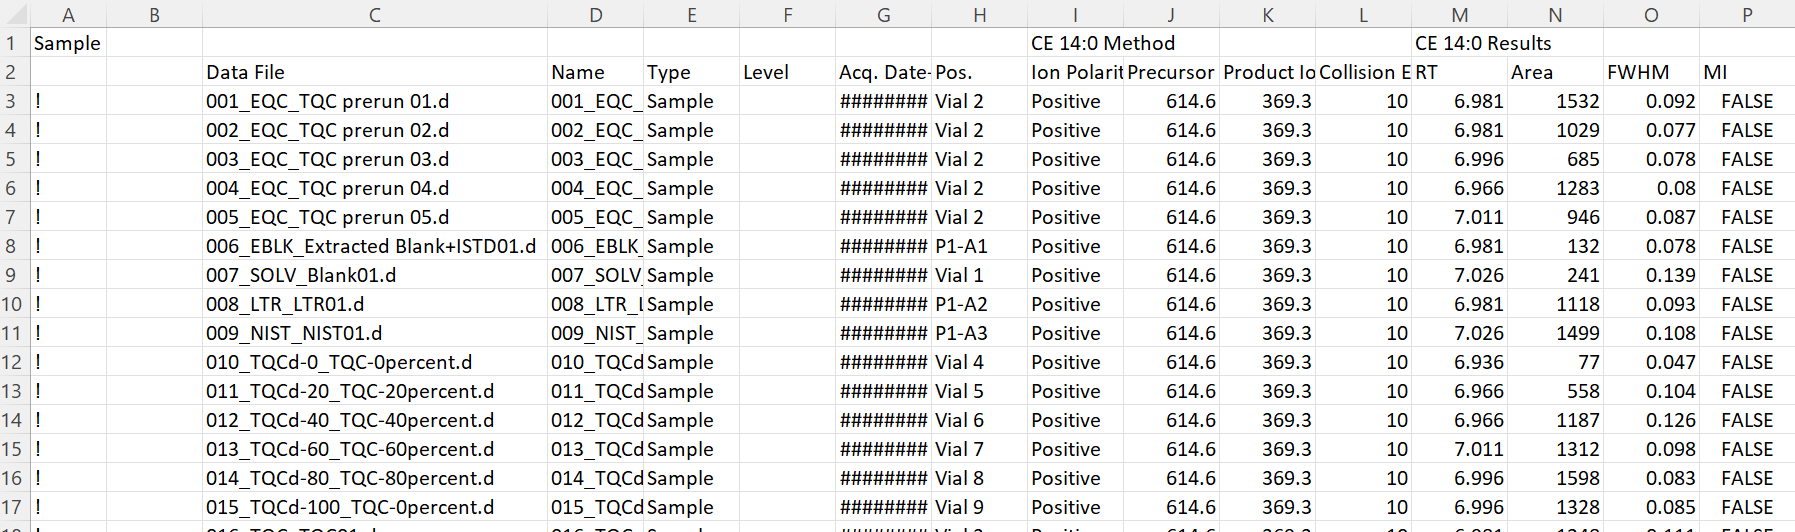
\includegraphics{./images/paste-A1421EC0.png}

\begin{Shaded}
\begin{Highlighting}[]
\NormalTok{data\_file\_path }\OtherTok{\textless{}{-}}\NormalTok{ here}\SpecialCharTok{::}\FunctionTok{here}\NormalTok{(}\StringTok{"data/Testdata\_Lipidomics\_MHQuant\_Detailed\_V2.csv"}\NormalTok{)}
\NormalTok{d\_all\_long }\OtherTok{\textless{}{-}}\NormalTok{ SLINGtools}\SpecialCharTok{::}\FunctionTok{read\_MassHunterCSV}\NormalTok{(data\_file\_path)}
\end{Highlighting}
\end{Shaded}

\begin{verbatim}
Reading 'Testdata_Lipidomics_MHQuant_Detailed_V2.csv' ... 

indexing Testdata_Lipidomics_MHQuant_Detailed_V2.csv [======] 2.15GB/s, eta:  0s
                                                                                
Imported  215 samples with 428 transitions 
\end{verbatim}

\begin{Shaded}
\begin{Highlighting}[]
\FunctionTok{print}\NormalTok{(d\_all\_long)}
\end{Highlighting}
\end{Shaded}

\begin{verbatim}
# A tibble: 92,020 x 14
   DataFileName     DataName SampleType AcqTimeStamp        VialPosition Feature
   <chr>            <chr>    <chr>      <dttm>              <chr>        <chr>  
 1 001_EQC_TQC pre~ 001_EQC~ EQC        2018-04-12 18:28:00 Vial 2       CE 14:0
 2 001_EQC_TQC pre~ 001_EQC~ EQC        2018-04-12 18:28:00 Vial 2       CE 15:0
 3 001_EQC_TQC pre~ 001_EQC~ EQC        2018-04-12 18:28:00 Vial 2       CE 16:0
 4 001_EQC_TQC pre~ 001_EQC~ EQC        2018-04-12 18:28:00 Vial 2       CE 16:1
 5 001_EQC_TQC pre~ 001_EQC~ EQC        2018-04-12 18:28:00 Vial 2       CE 16:2
 6 001_EQC_TQC pre~ 001_EQC~ EQC        2018-04-12 18:28:00 Vial 2       CE 17:0
 7 001_EQC_TQC pre~ 001_EQC~ EQC        2018-04-12 18:28:00 Vial 2       CE 17:1
 8 001_EQC_TQC pre~ 001_EQC~ EQC        2018-04-12 18:28:00 Vial 2       CE 18:0
 9 001_EQC_TQC pre~ 001_EQC~ EQC        2018-04-12 18:28:00 Vial 2       CE 18:1
10 001_EQC_TQC pre~ 001_EQC~ EQC        2018-04-12 18:28:00 Vial 2       CE 18:~
# ... with 92,010 more rows, and 8 more variables: IonPolarity <fct>,
#   PrecursorMZ <dbl>, ProductMZ <dbl>, CollisionEnergy <dbl>, RT <dbl>,
#   Area <dbl>, FWHM <dbl>, MI <lgl>
\end{verbatim}

\bookmarksetup{startatroot}

\hypertarget{references}{%
\chapter*{References}\label{references}}
\addcontentsline{toc}{chapter}{References}

\hypertarget{refs}{}
\begin{CSLReferences}{0}{0}
\end{CSLReferences}



\end{document}
